\documentclass[9pt]{article}
\usepackage[left=.5in, right=.5in, top=1in]{geometry}

\usepackage{graphicx}					
\usepackage{amssymb}
\usepackage{float}
\usepackage{url}
\usepackage{graphicx}					
\usepackage{import}
\usepackage{dcolumn}
\usepackage{amssymb}
\usepackage{adjustbox}

\title{Foreign Aid and Soft Power}
\author{.}

% ------------------------------------------------------------------------------------
\begin{document}
\maketitle
\tableofcontents

\setlength{\tabcolsep}{5pt}

% ------------------------------------------------------------------------------------
\newpage
\section{Body of Paper}

\begin{figure}[H]
\centering
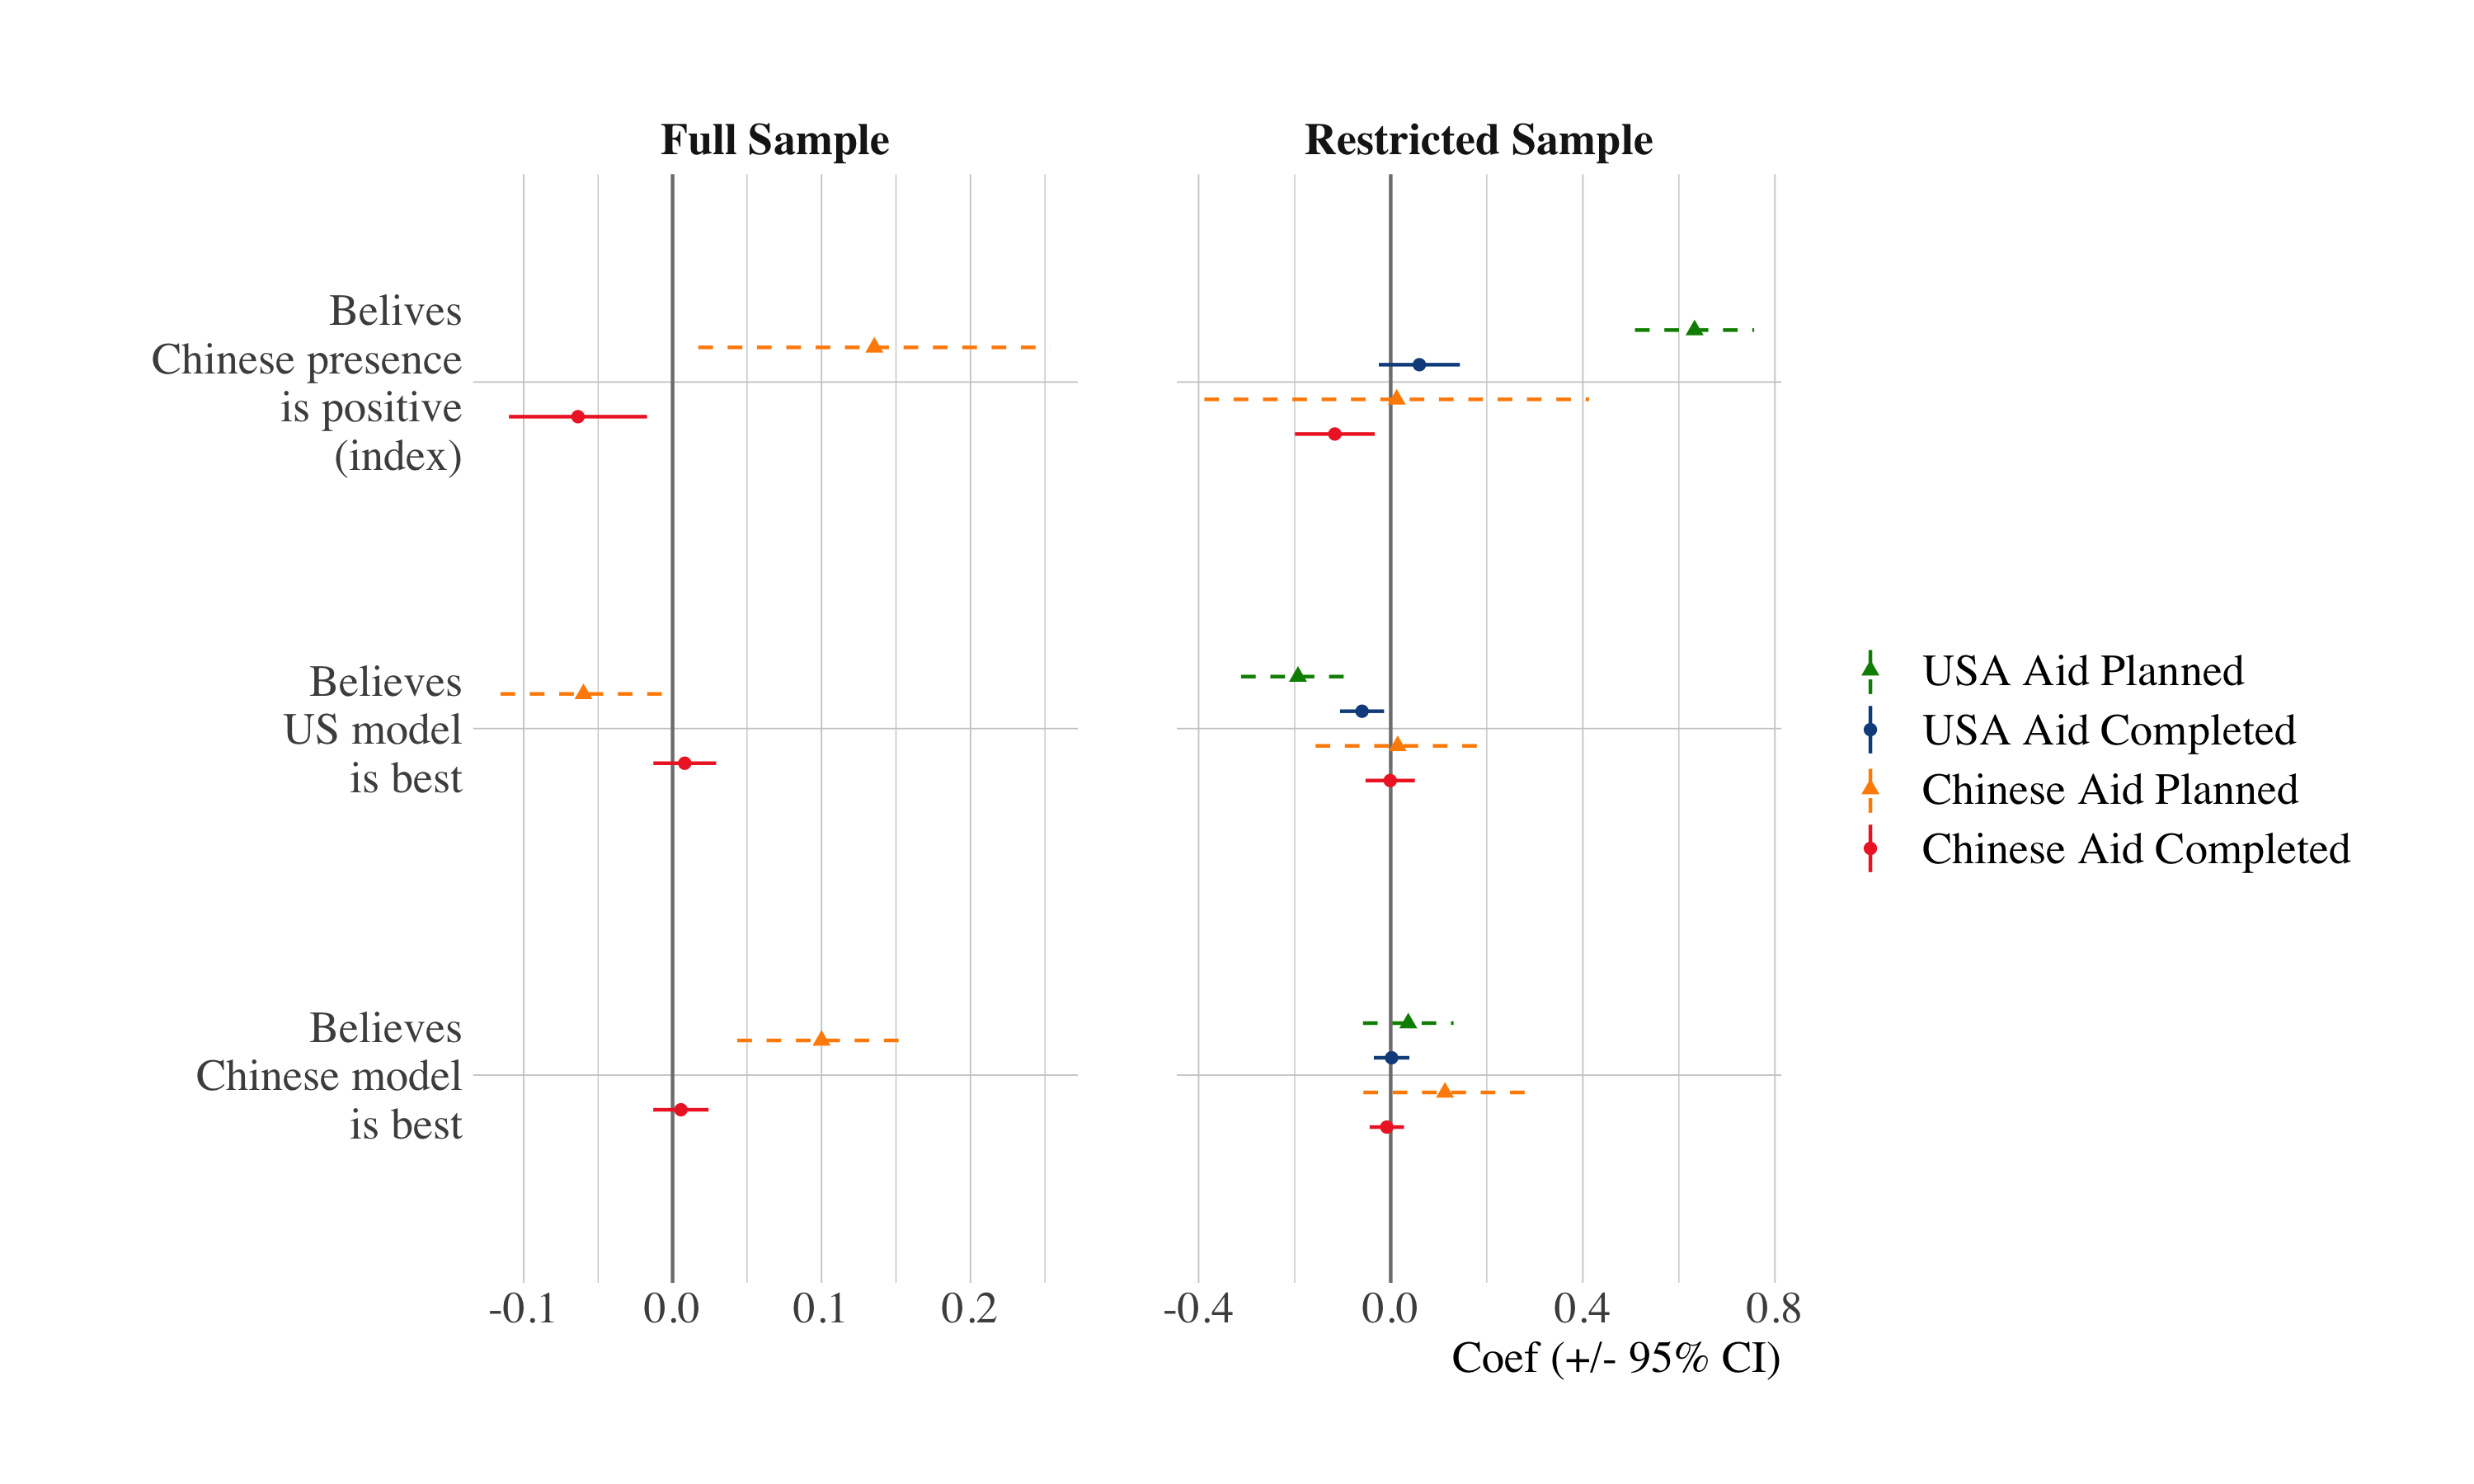
\includegraphics[width=1\textwidth]{figures/figure_01.png}
\caption{Effects of Chinese and US aid on perceptions of China and the US}
\end{figure}

\begin{figure}[H]
\centering
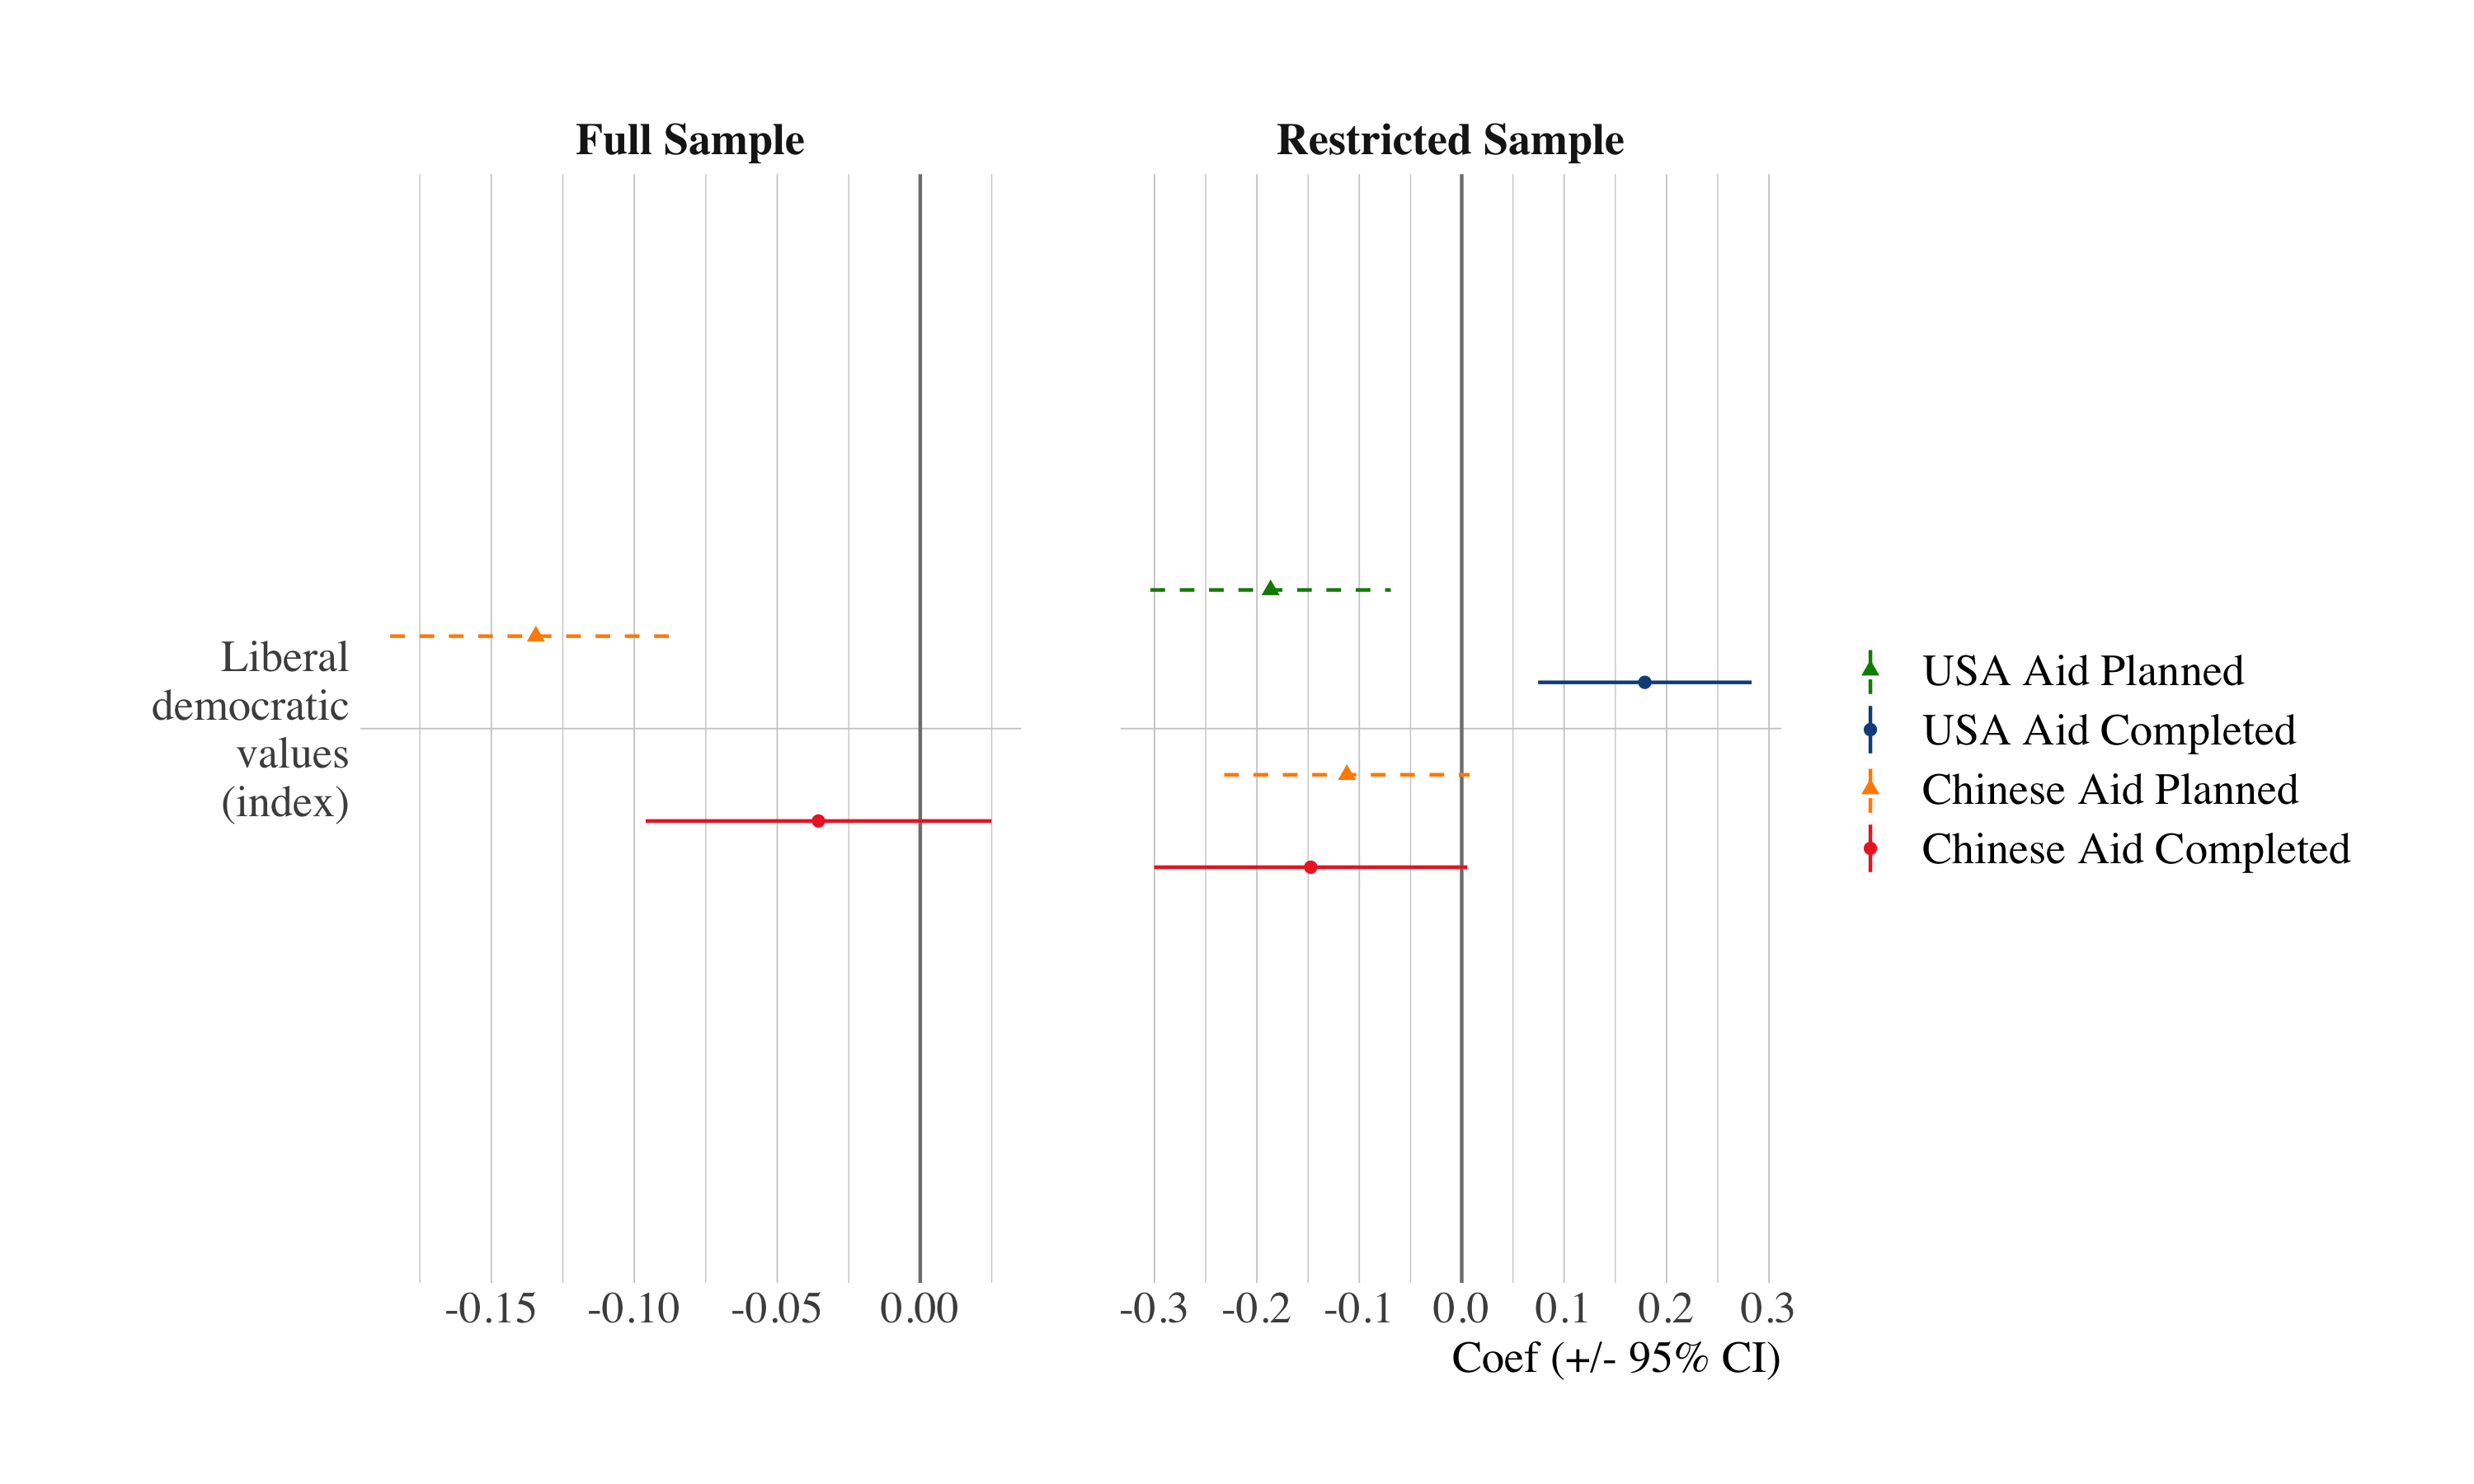
\includegraphics[width=1\textwidth]{figures/figure_02.png}
\caption{Effects of Chinese and US aid on liberal democratic values}
\end{figure}

\begin{figure}[H]
\centering
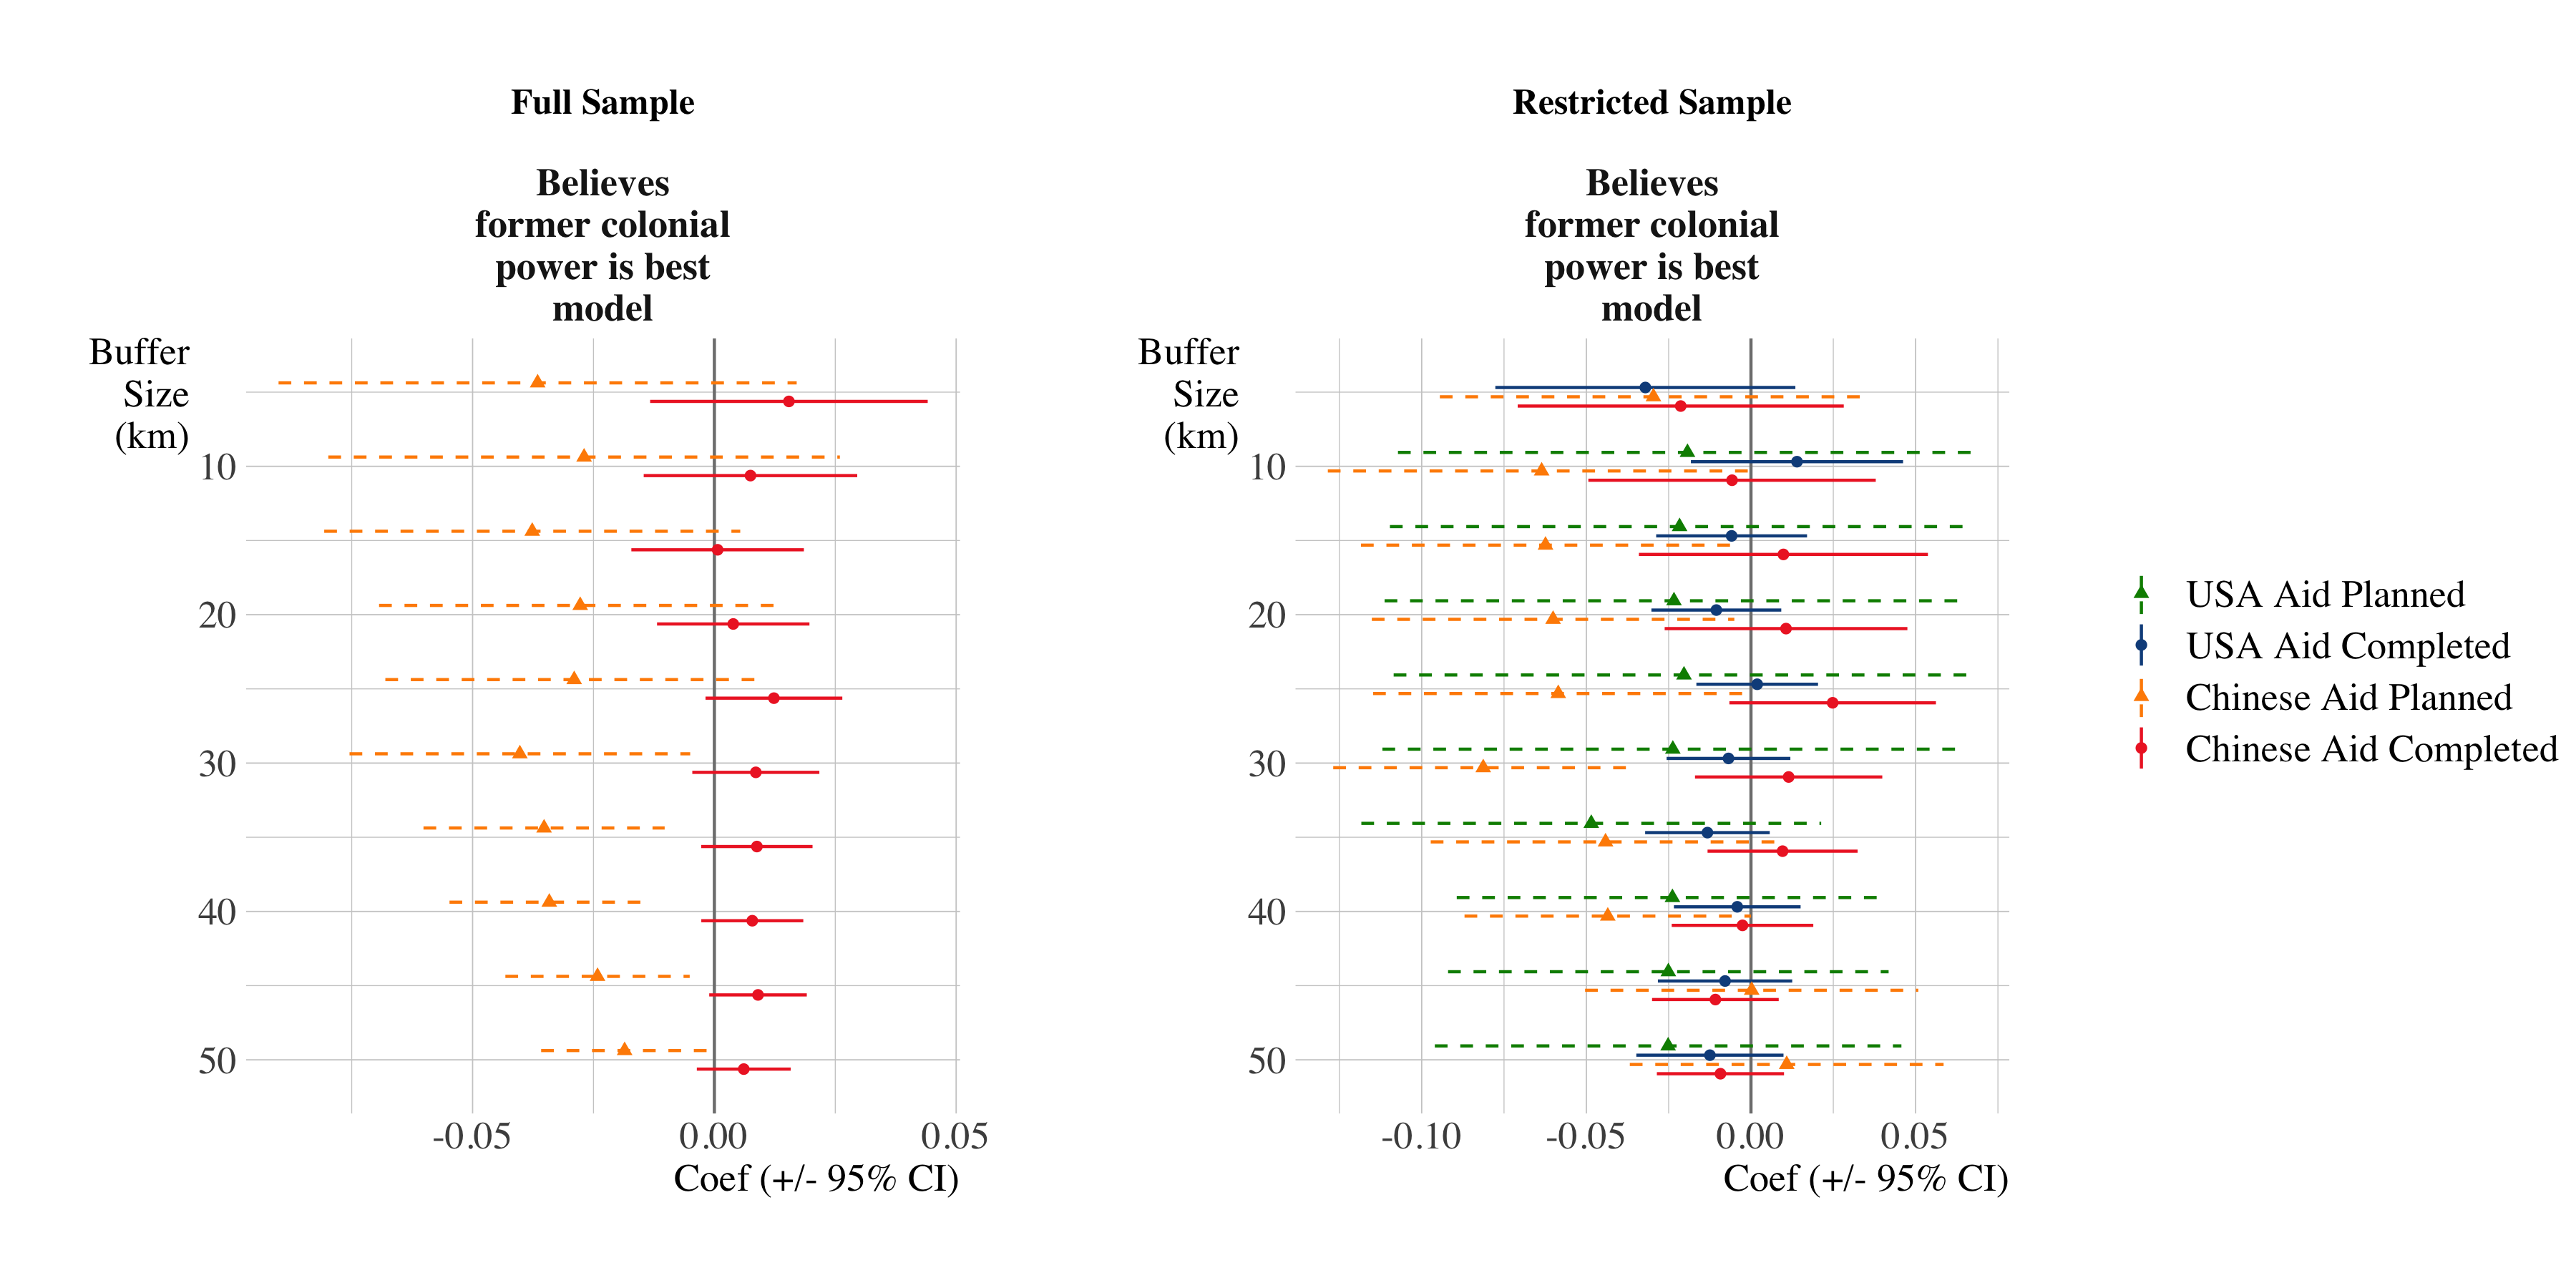
\includegraphics[width=1\textwidth]{figures/figure_03.png}
\caption{Effects of Chinese and US aid on perceptions of former colonial powers}
\end{figure}

\begin{figure}[H]
\centering
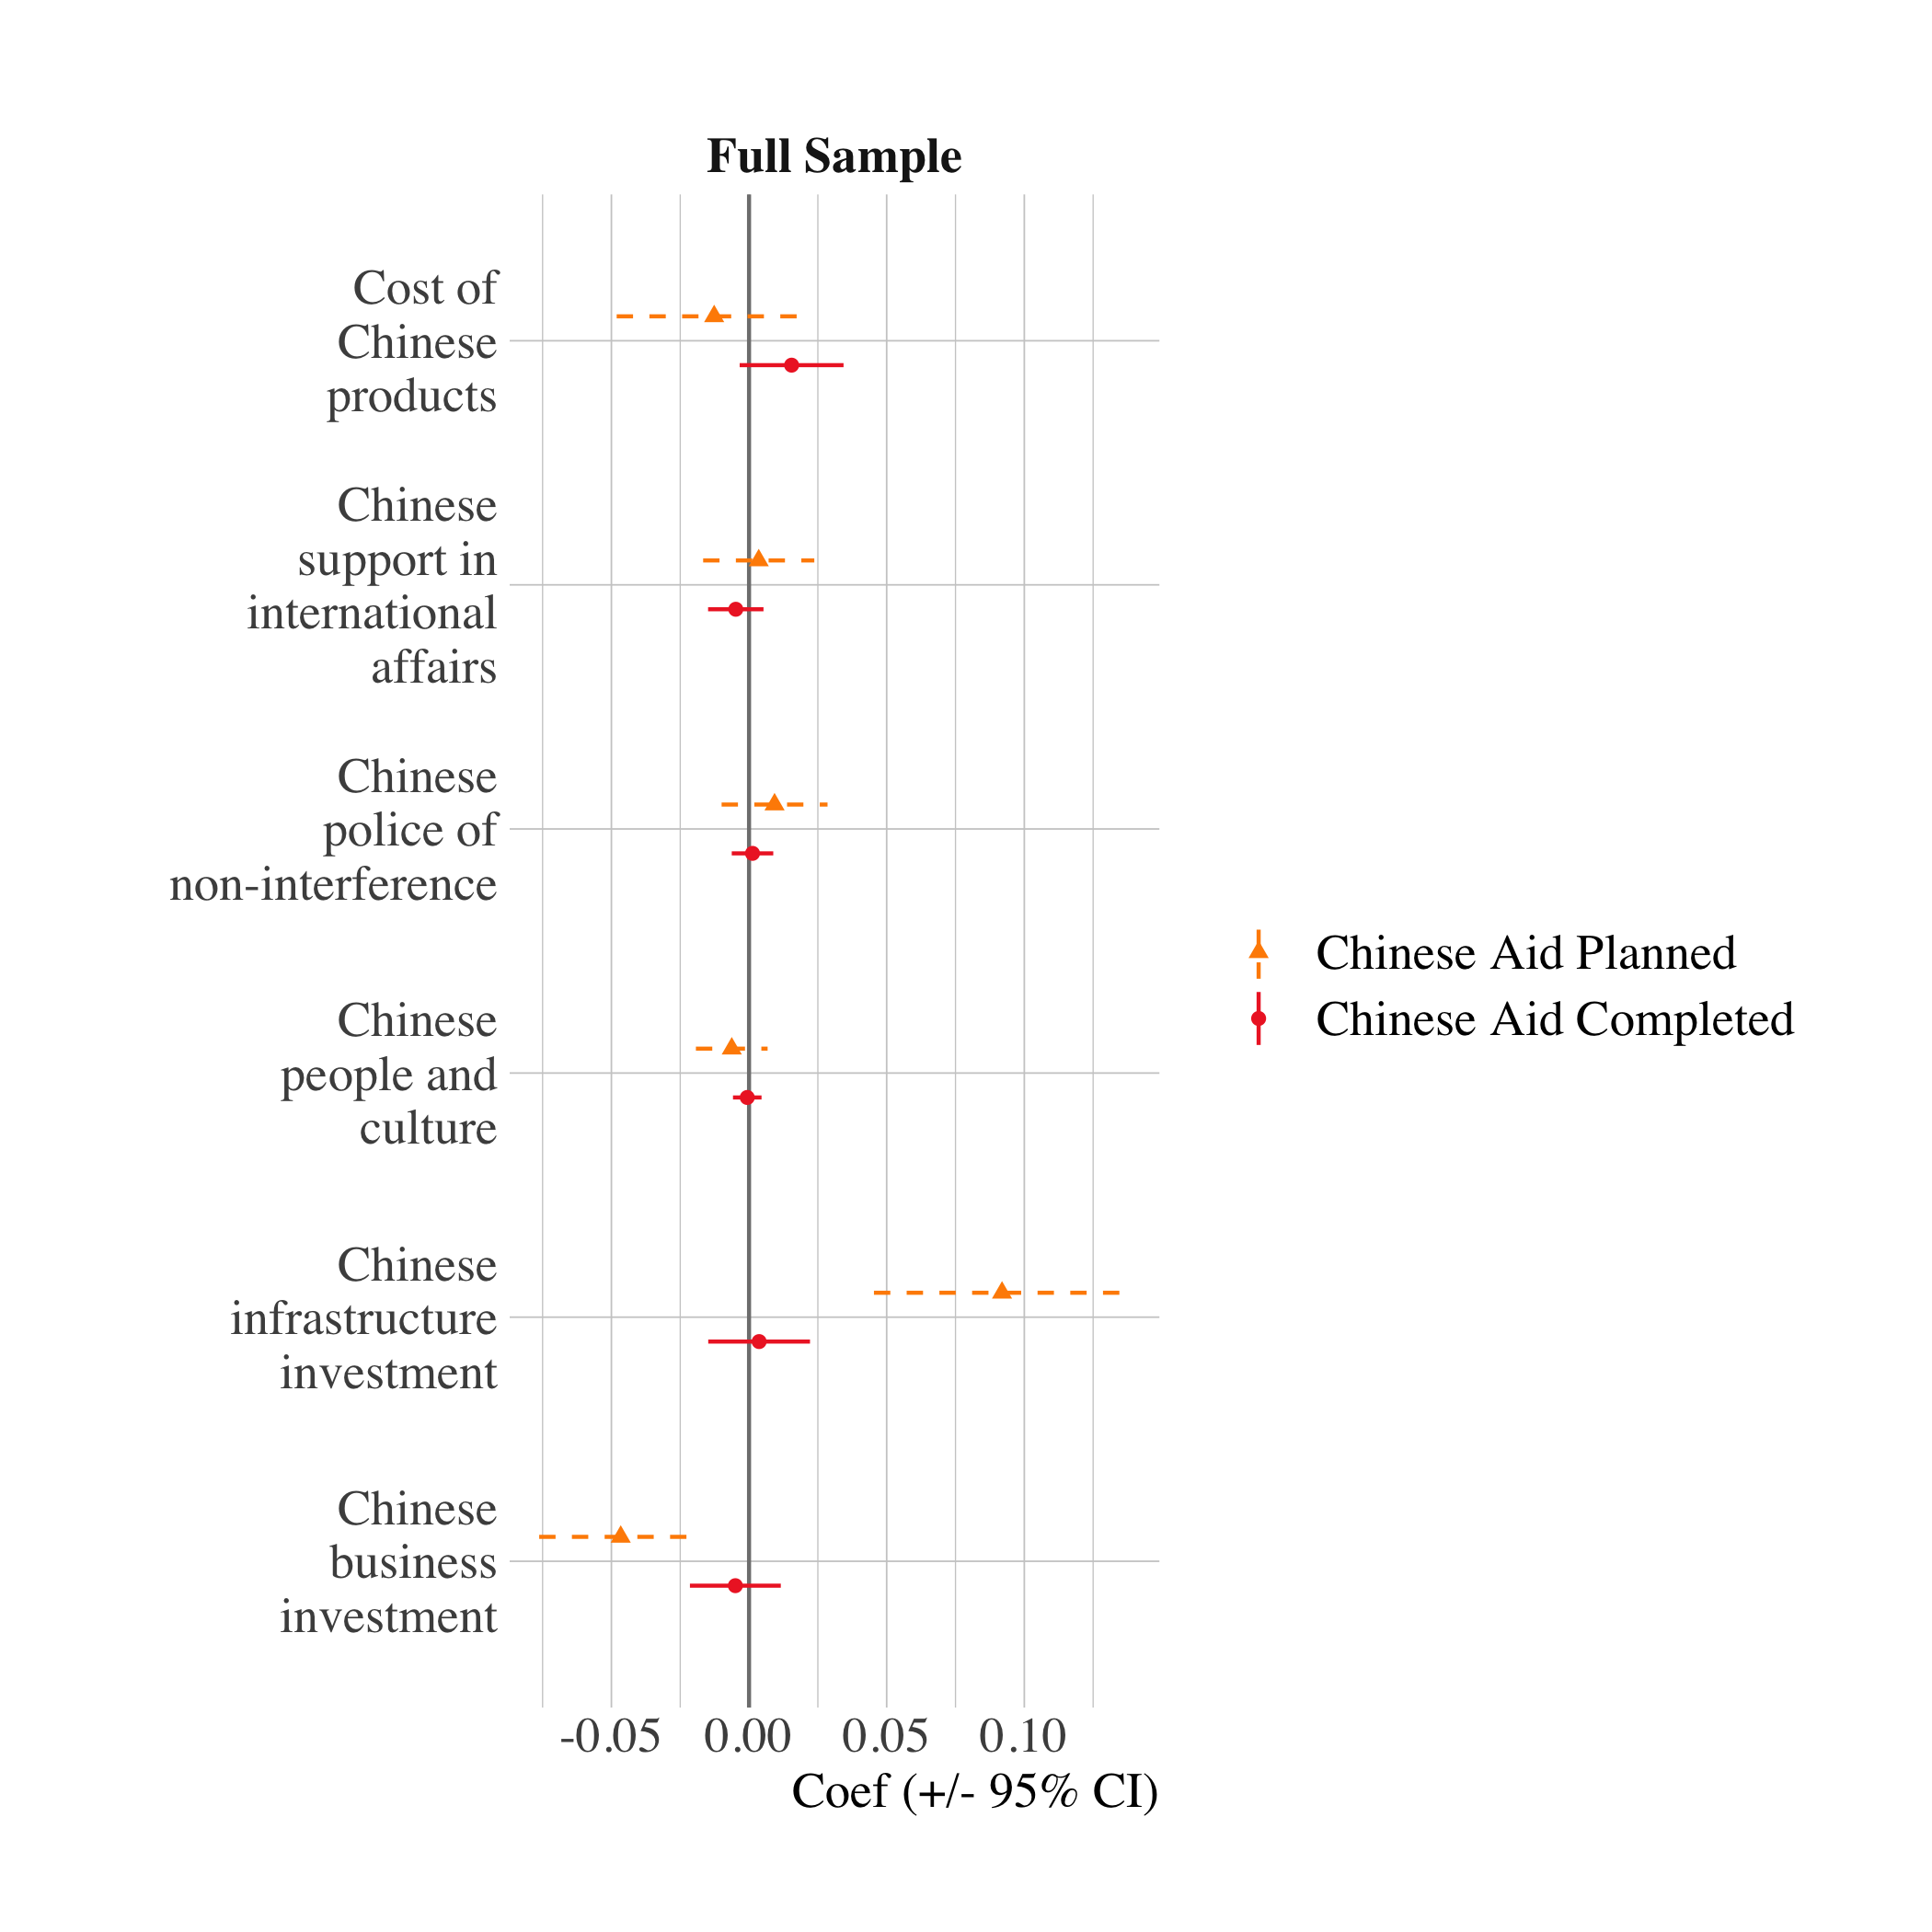
\includegraphics[width=0.8\textwidth]{figures/figure_04.png}
\caption{Effects of Chinese aid on factors contributing to positive image of China}
\end{figure}

\begin{figure}[H]
\centering
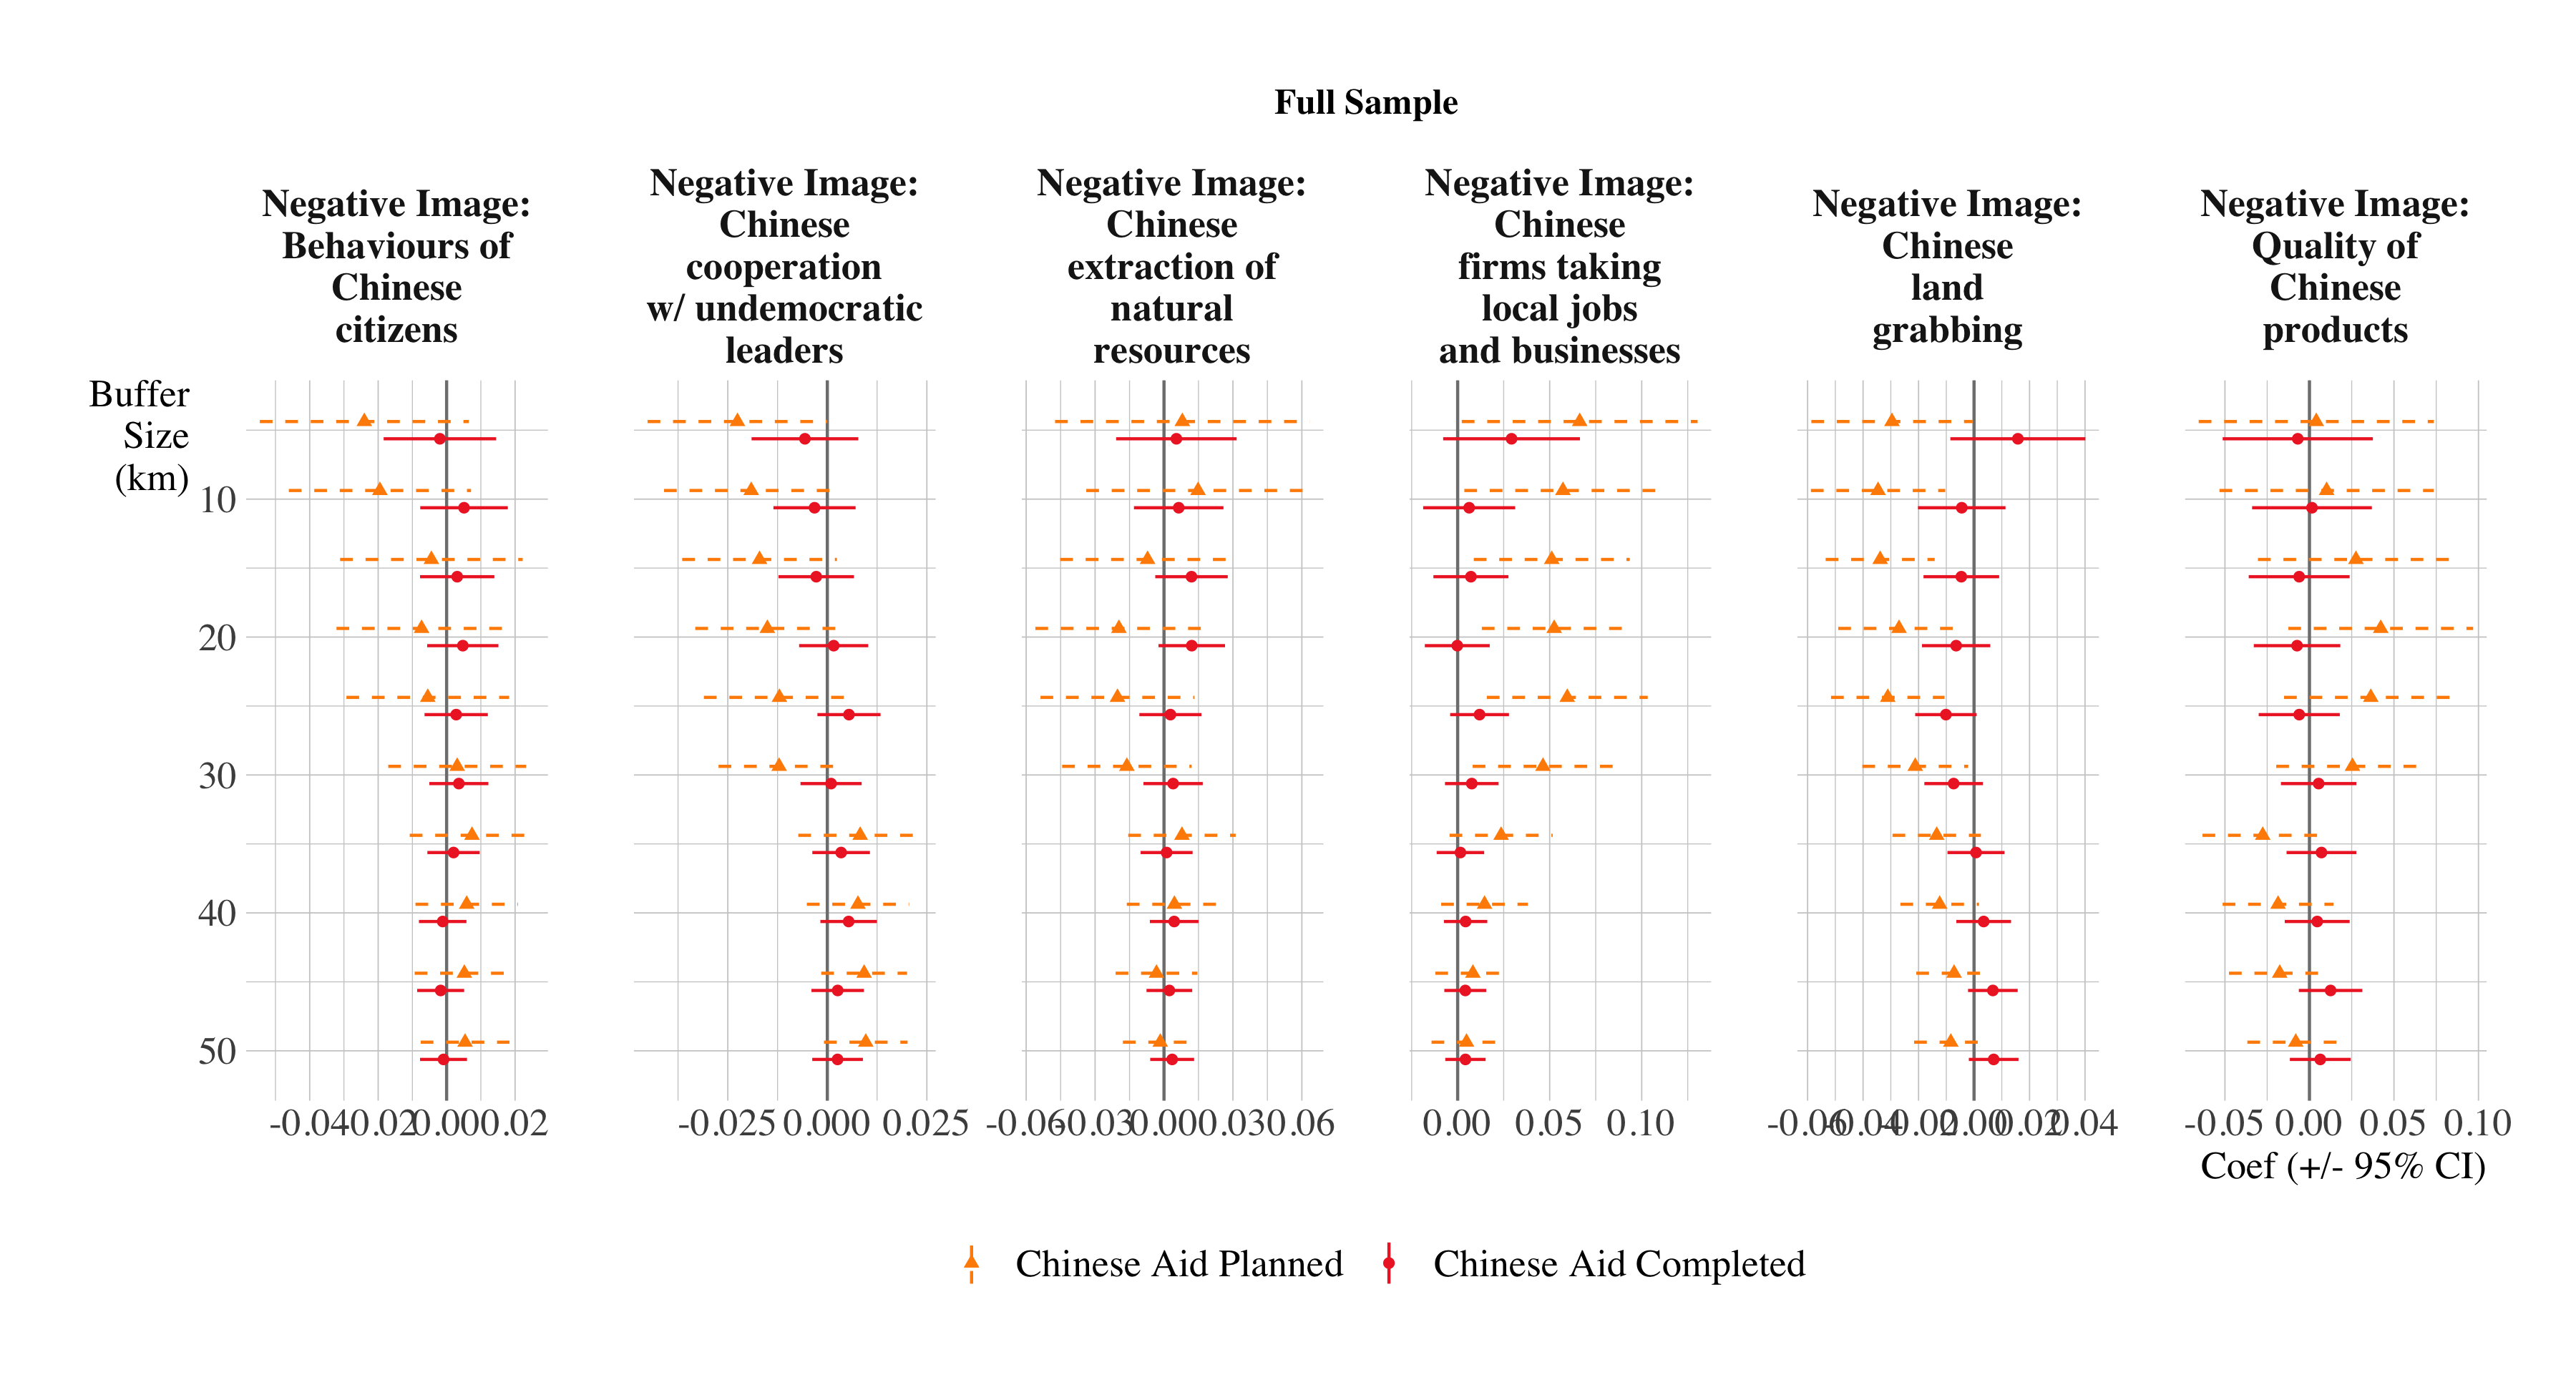
\includegraphics[width=0.8\textwidth]{figures/figure_05.png}
\caption{Effects of Chinese aid on factors contributing to negative image of China}
\end{figure}

% ------------------------------------------------------------------------------------
\renewcommand\thefigure{A\arabic{figure}}    
\renewcommand\thetable{A\arabic{table}}    

\setcounter{figure}{0} 
\setcounter{table}{0} 

\newpage
\appendix
\section{Appendix 1: Coding Rules and Descriptive Statistics}

\begin{figure}[H]
\centering
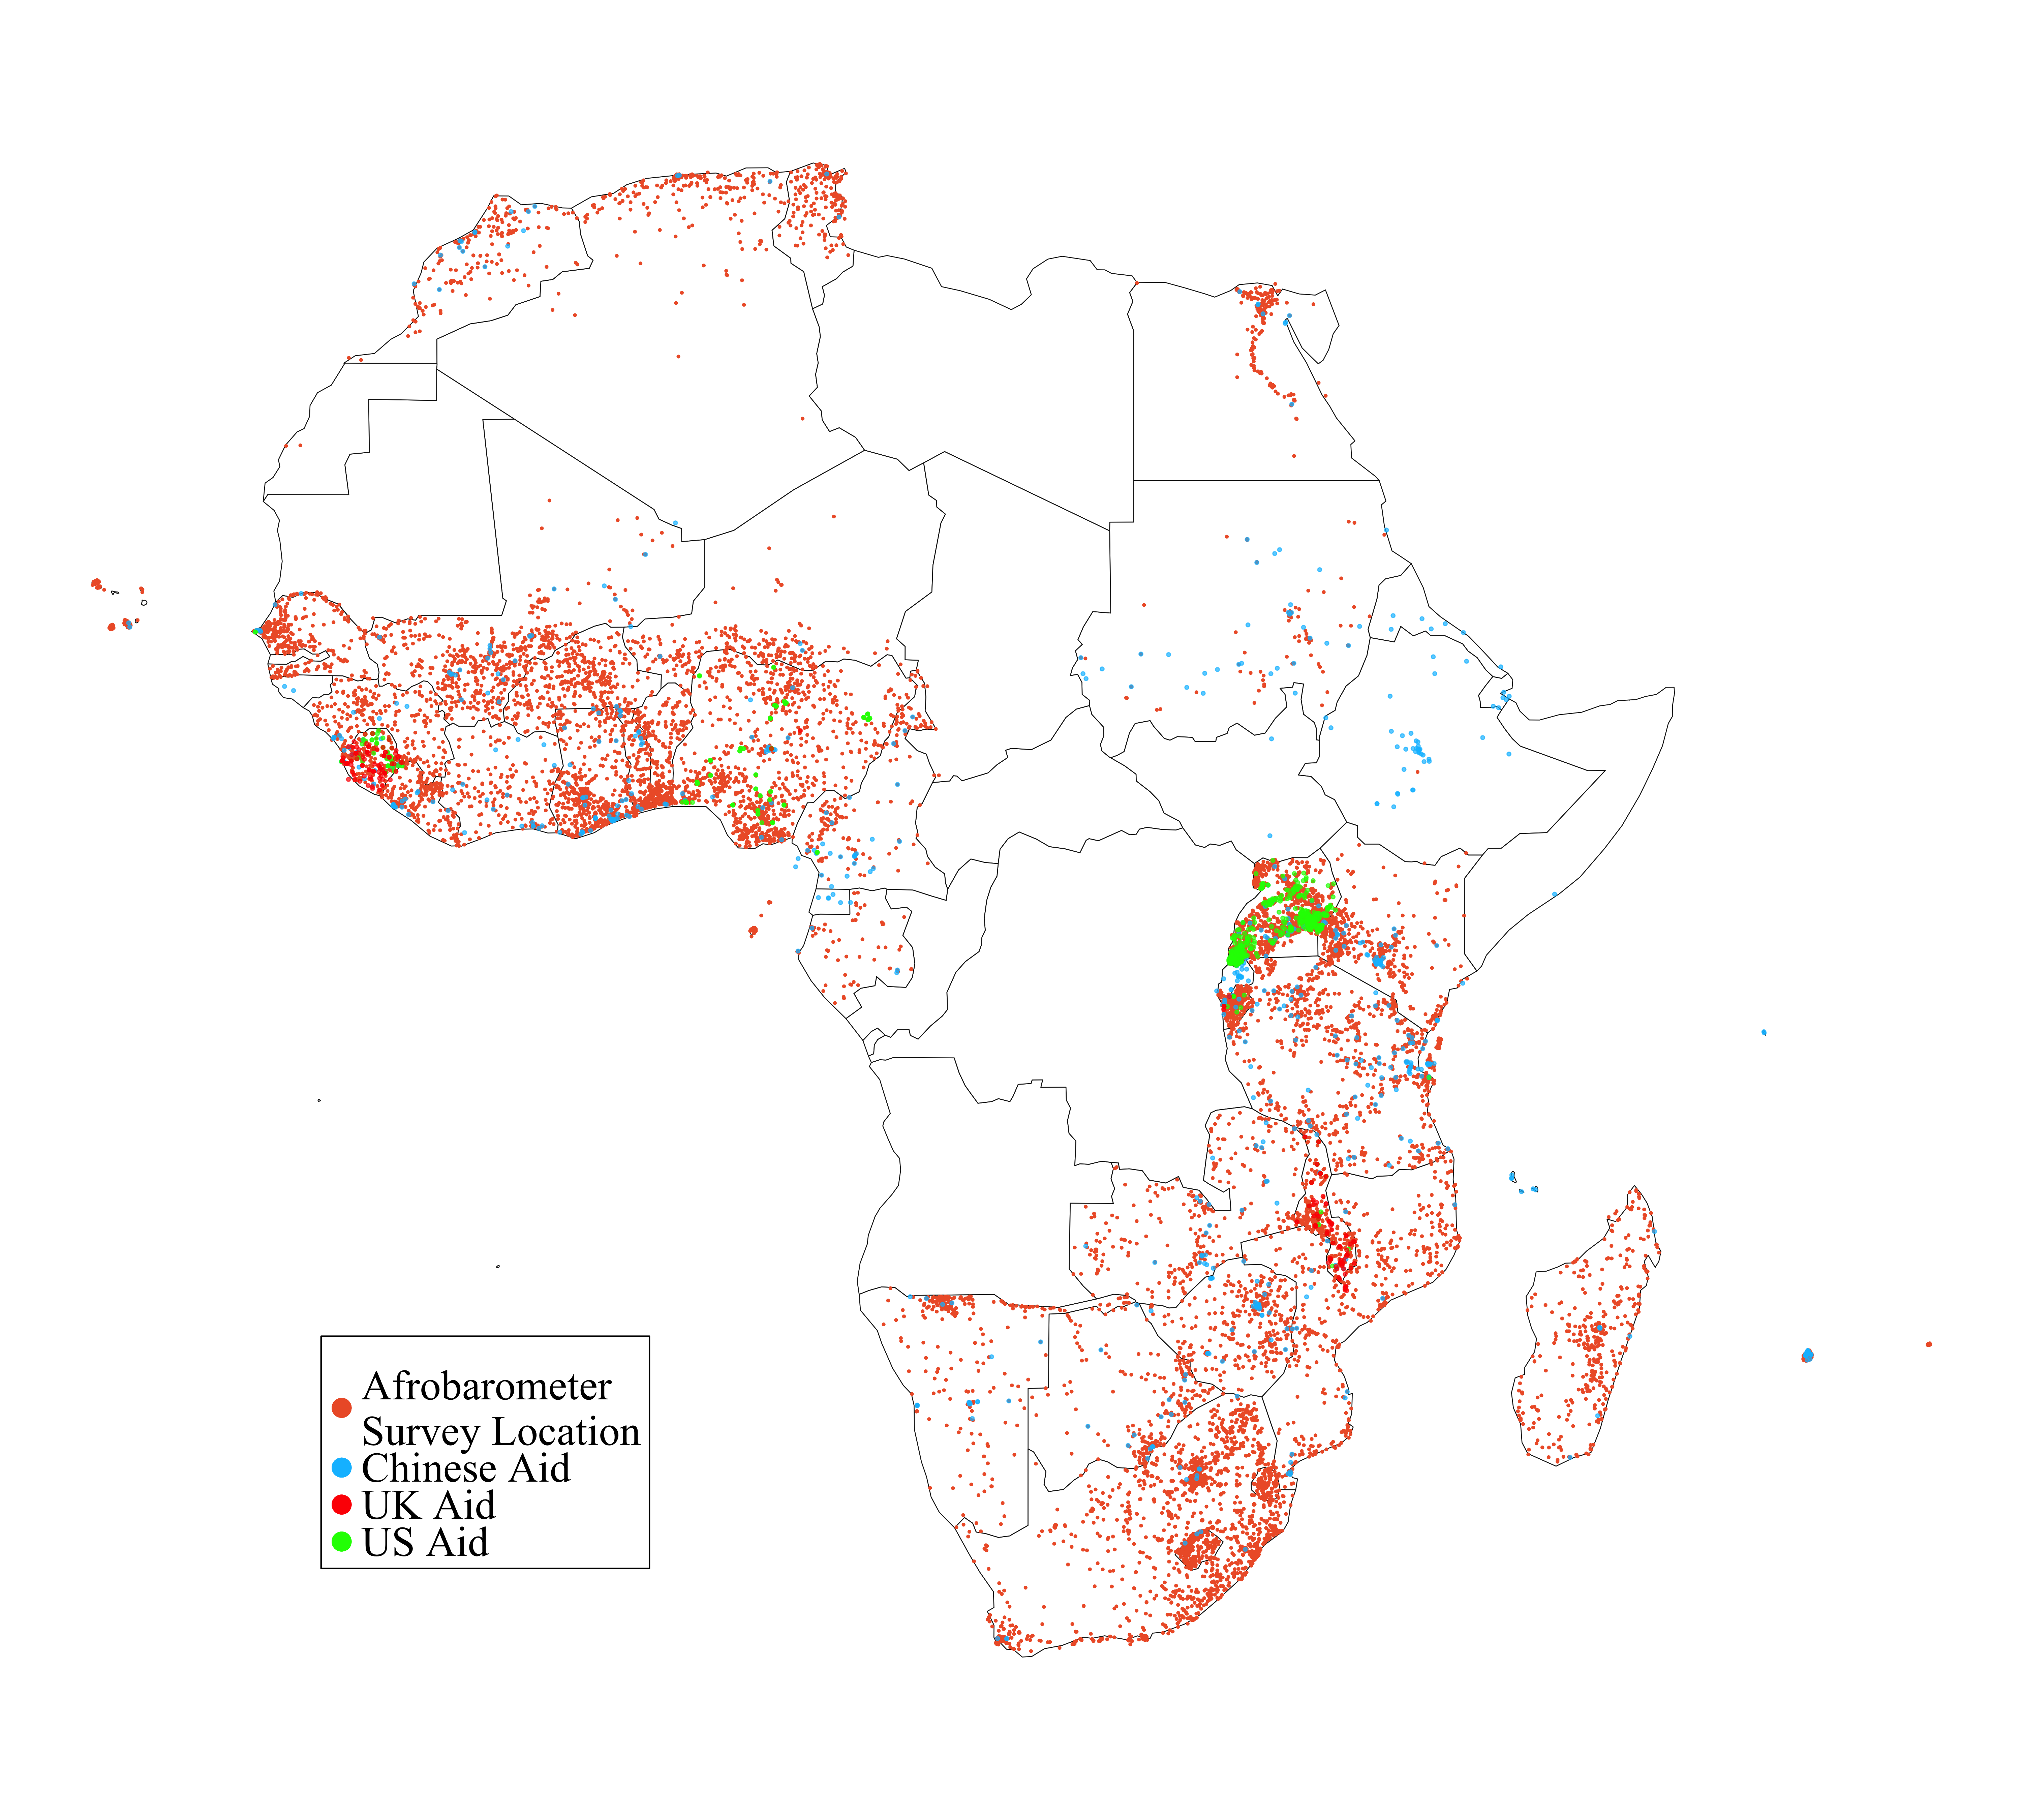
\includegraphics[width=1\textwidth]{figures/figure_a1.png}
\caption{Map of Afrobarometer respondents and Chinese, US, and UK aid projects}
\end{figure}

\begin{figure}[H]
\centering
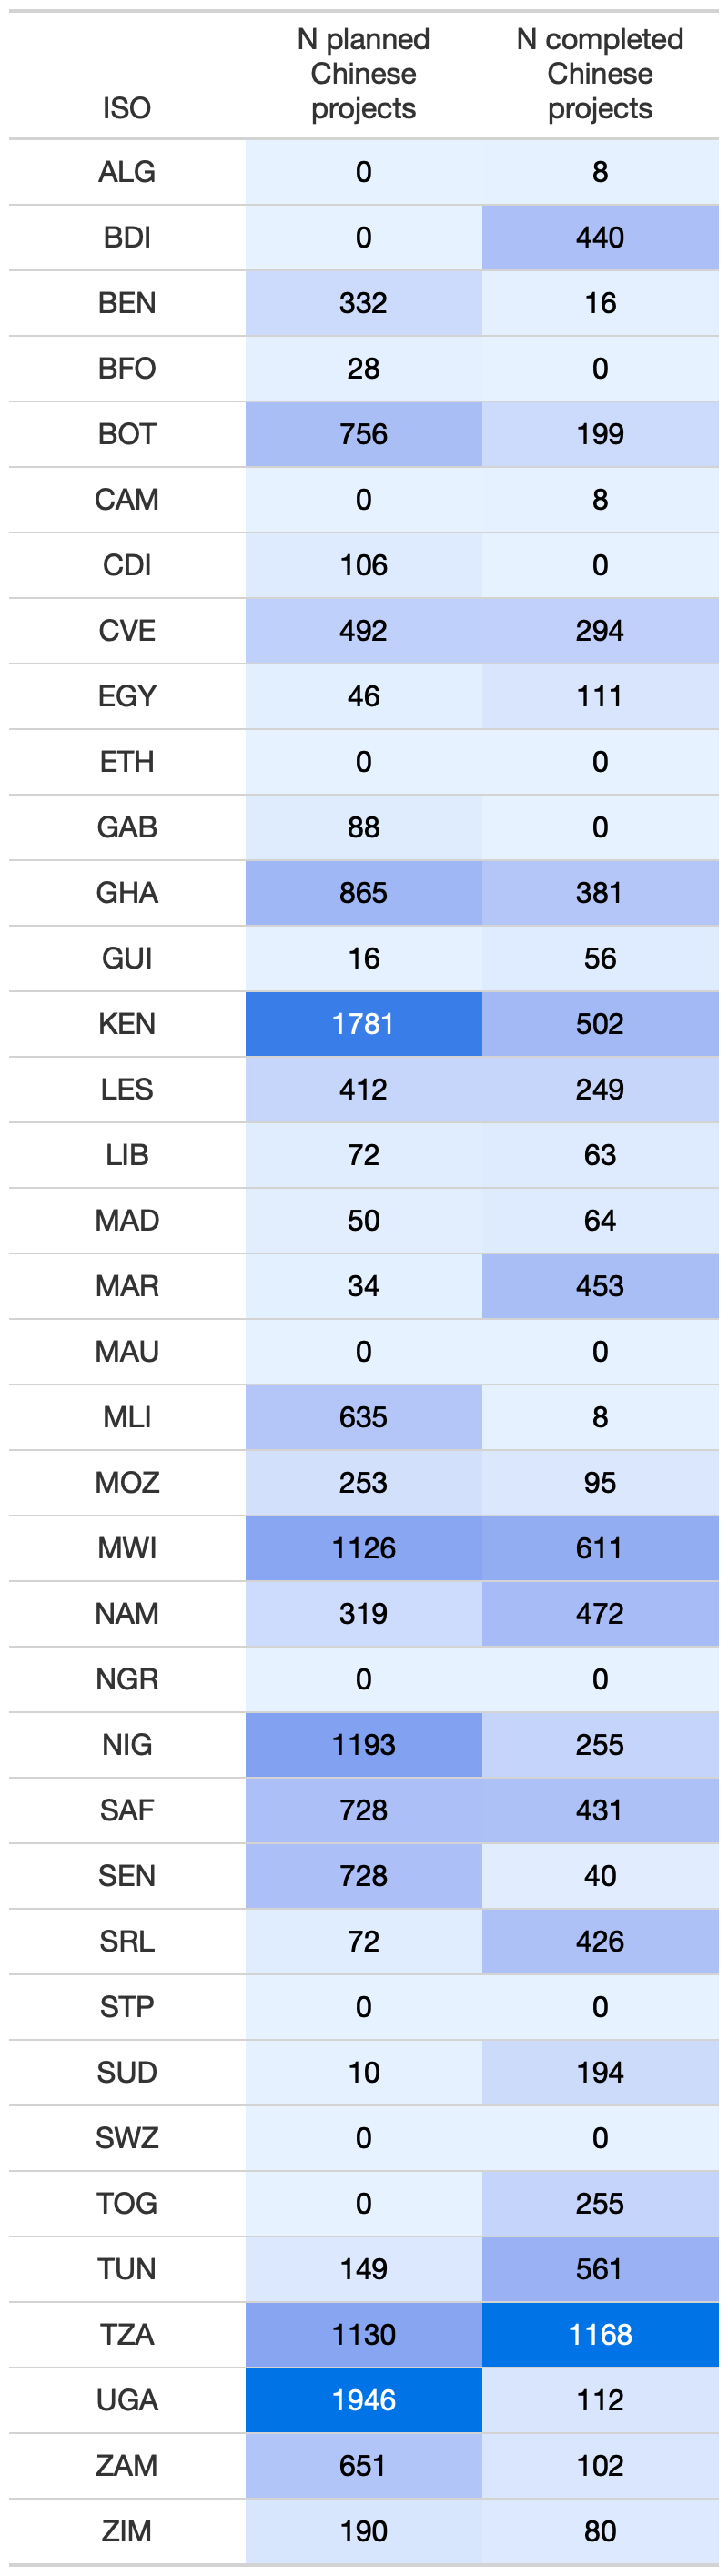
\includegraphics[width=0.3\textwidth]{figures/figure_a2.png}
\caption{Distribution of Chinese projects by country in full sample}
\end{figure}

\begin{figure}[H]
\centering
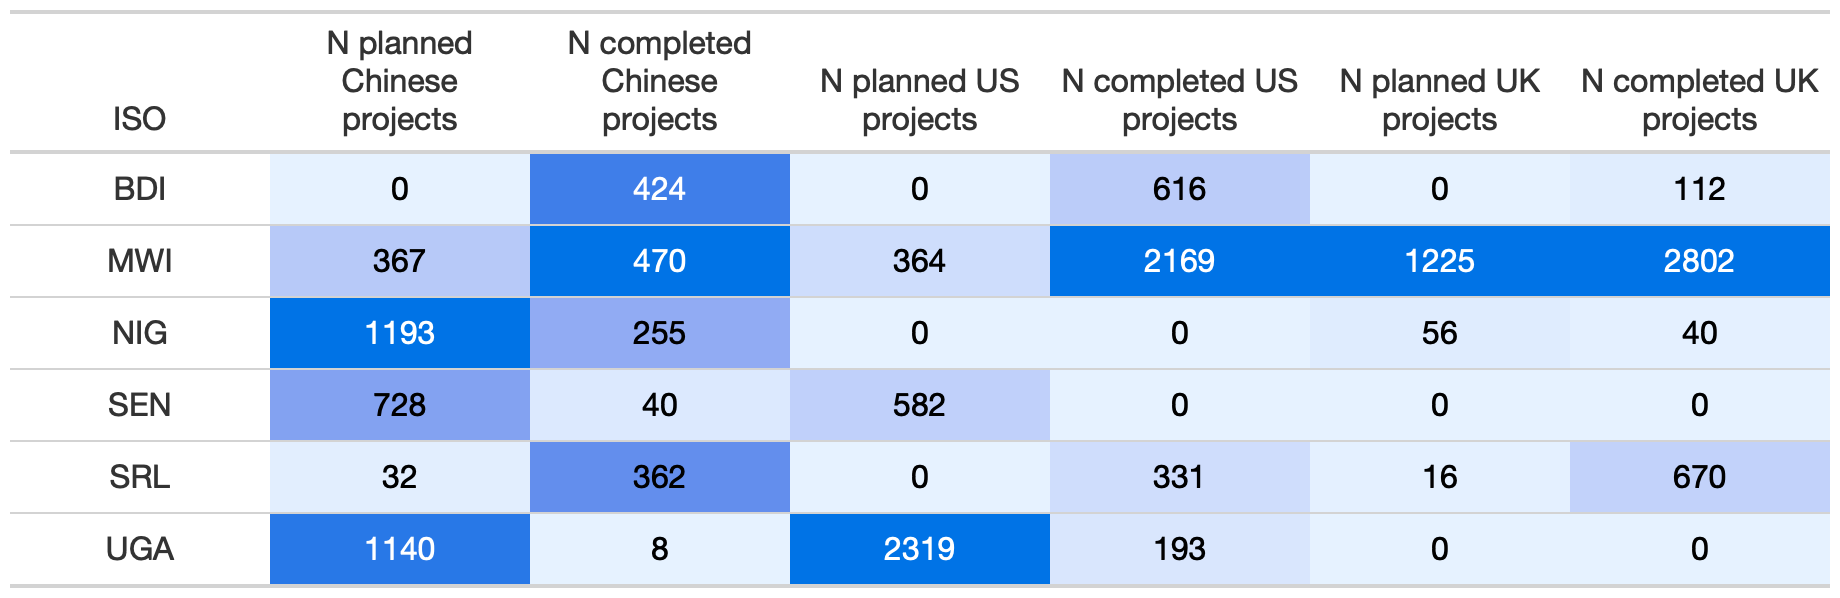
\includegraphics[width=0.7\textwidth]{figures/figure_a3.png}
\caption{Distribution of Chinese, US, and UK projects by country in restricted sample}
\end{figure}

\setlength{\tabcolsep}{5pt}
\begin{table}[H]
\caption{Descriptive statistics on independent variables}
\label{reg}
\centering
\import{tables/}{table_a1.tex}
\end{table}

\setlength{\tabcolsep}{5pt}
\begin{table}[H]
\caption{Descriptive statistics on dependent variables}
\label{reg}
\centering
\import{tables/}{table_a2.tex}
\end{table}

\setlength{\tabcolsep}{5pt}
\begin{table}[H]
\caption{Descriptive statistics on control variables}
\label{reg}
\centering
\import{tables/}{table_a3.tex}
\end{table}

\setlength{\tabcolsep}{5pt}
\begin{table}[H]
\caption{Comparison of Chinese projects in full sample and our sample by sector}
\label{reg}
\centering
\import{tables/}{table_a4.tex}
\end{table}

\setlength{\tabcolsep}{5pt}
\begin{table}[H]
\caption{Comparison of US projects in full sample and our sample by sector}
\label{reg}
\centering
\import{tables/}{table_a5.tex}
\end{table}

\setlength{\tabcolsep}{5pt}
\begin{table}[H]
\caption{Comparison of completed and planned Chinese projects by sector}
\label{reg}
\centering
\import{tables/}{table_a6.tex}
\end{table}

\setlength{\tabcolsep}{5pt}
\begin{table}[H]
\caption{Comparison of completed and planned US projects by sector}
\label{reg}
\centering
\import{tables/}{table_a7.tex}
\end{table}

\setlength{\tabcolsep}{5pt}
\begin{table}[H]
\caption{Correlation between survey- and AidData-based proxies for Chinese aid in rural Liberia}
\label{reg}
\centering
%\import{tables/}{table_a8.tex}
\end{table}

% ------------------------------------------------------------------------------------
\newpage
\section{Appendix 2: Robustness Checks}

\begin{figure}[H]
\centering
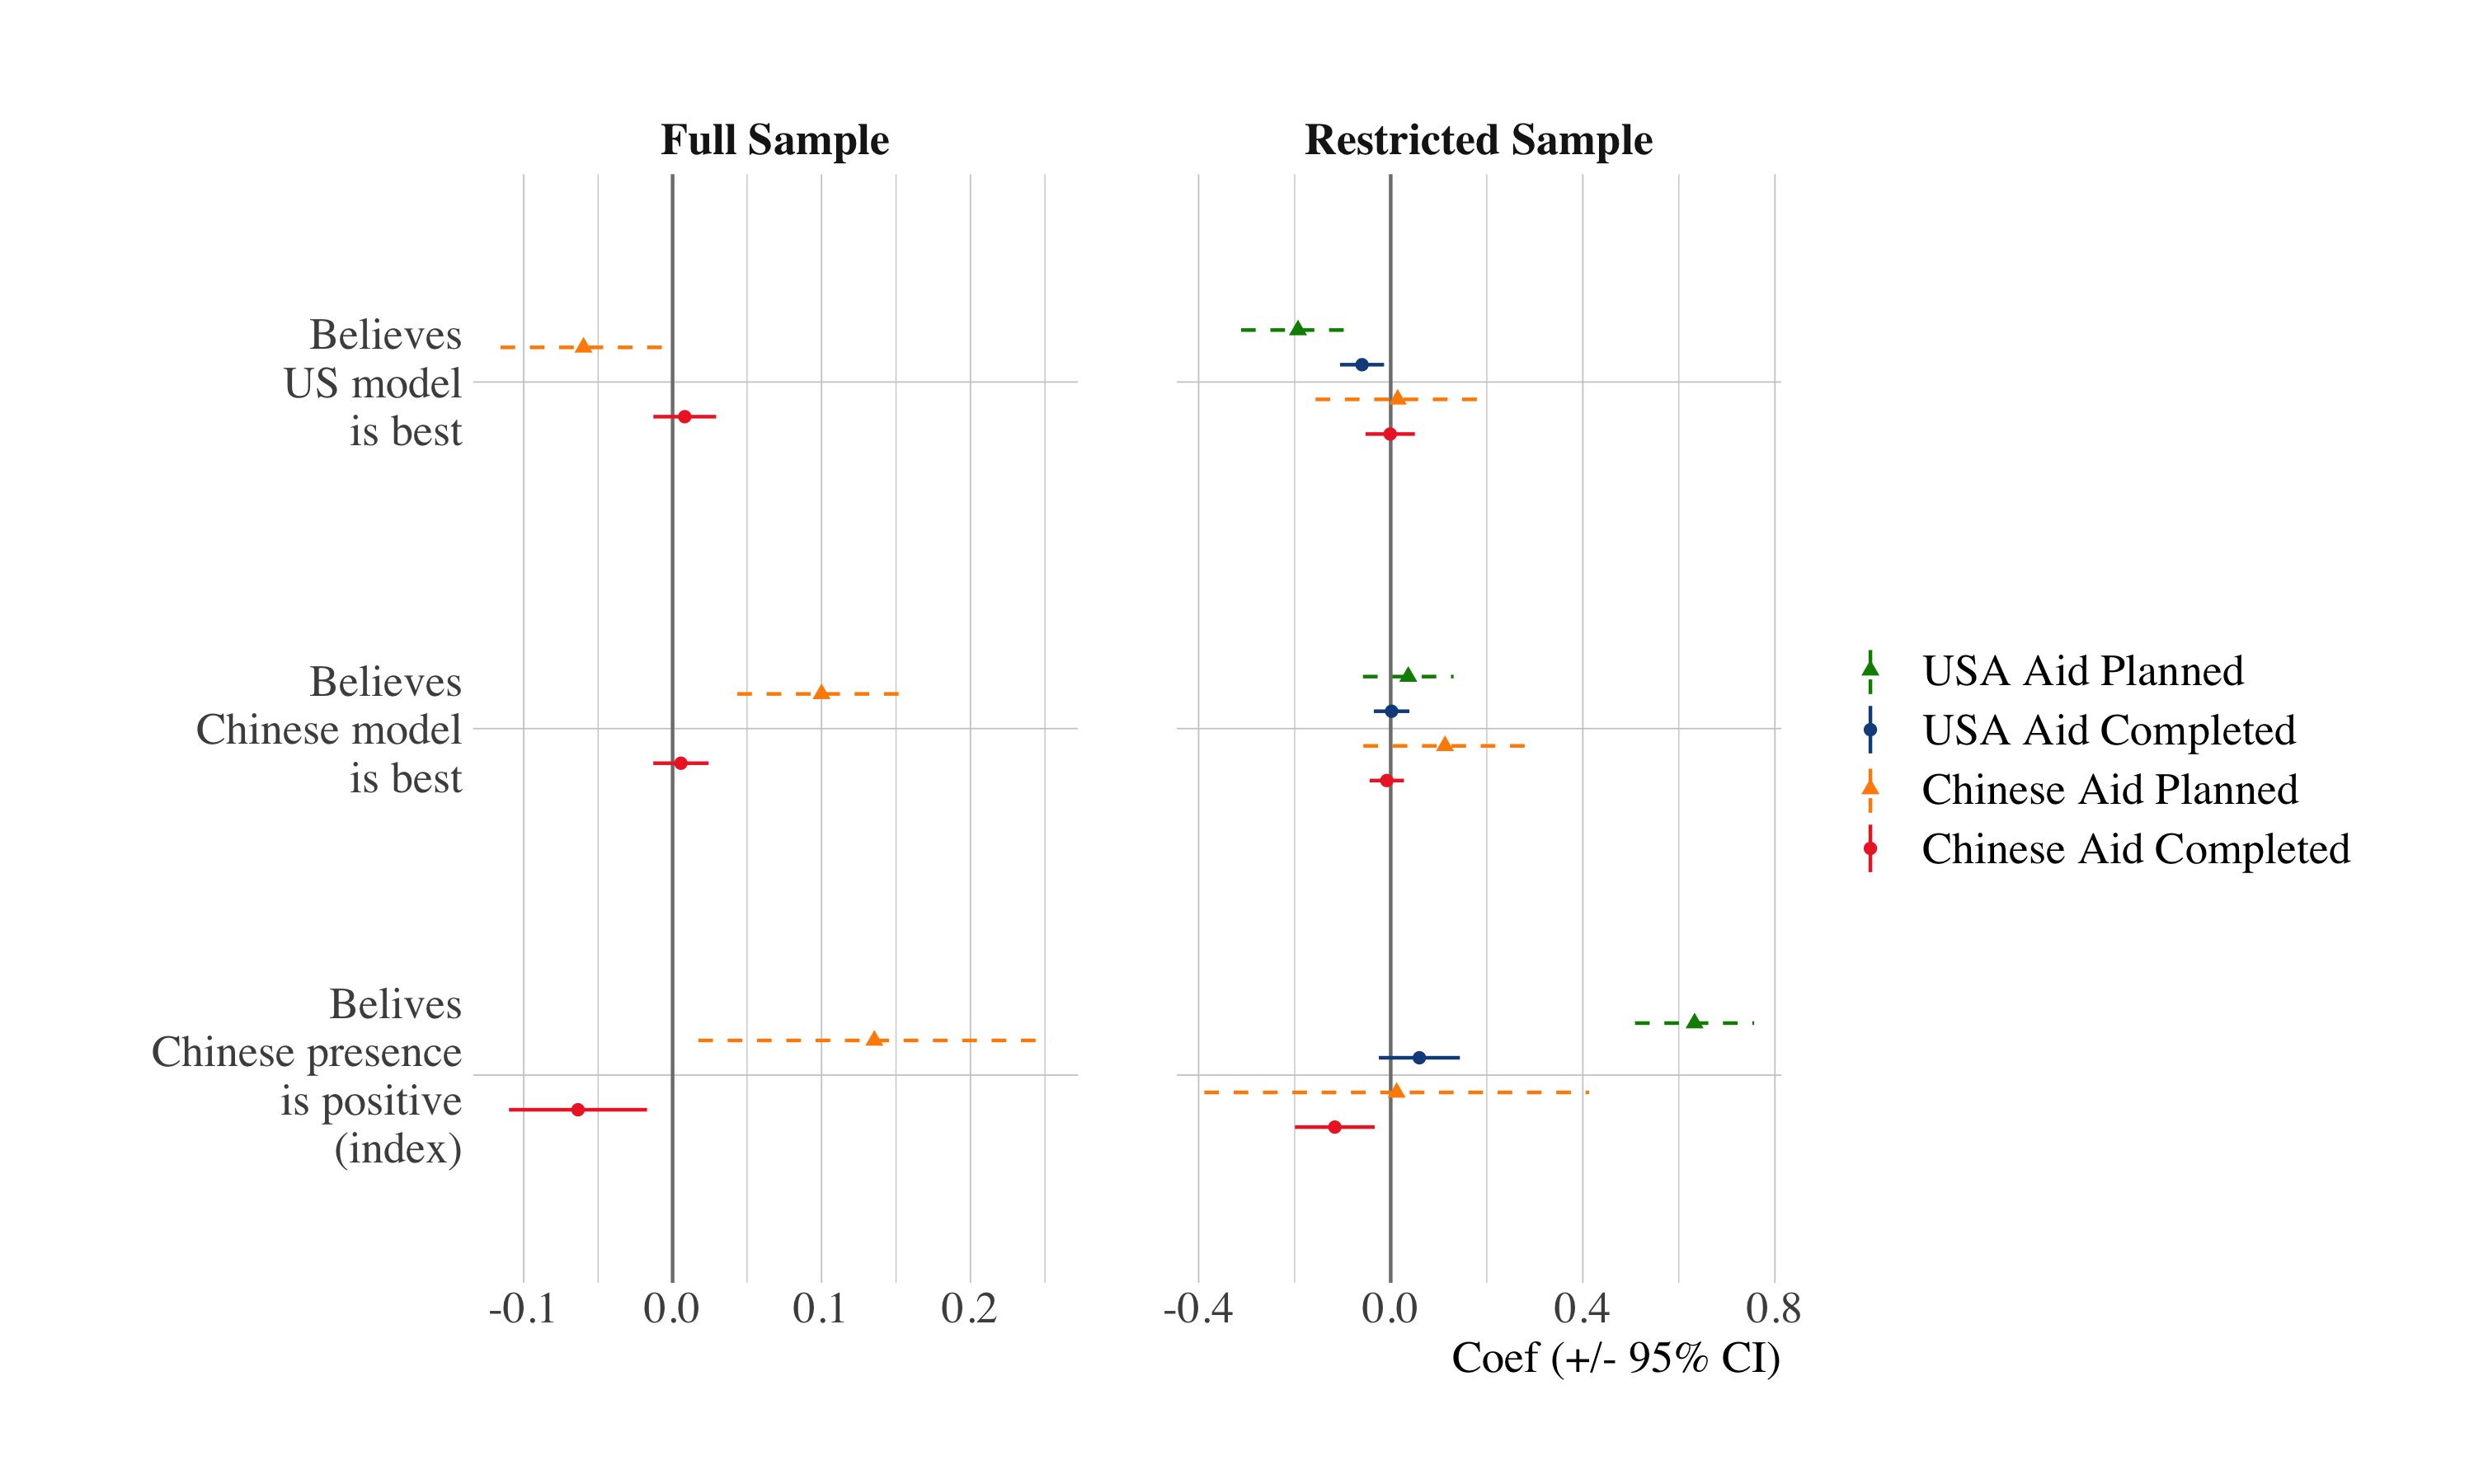
\includegraphics[width=1\textwidth]{figures/figure_a4.png}
\caption{Effects of Chinese and US aid on perceptions of China and the US, using 2008 as cutoff year}
\end{figure}

\begin{figure}[H]
\centering
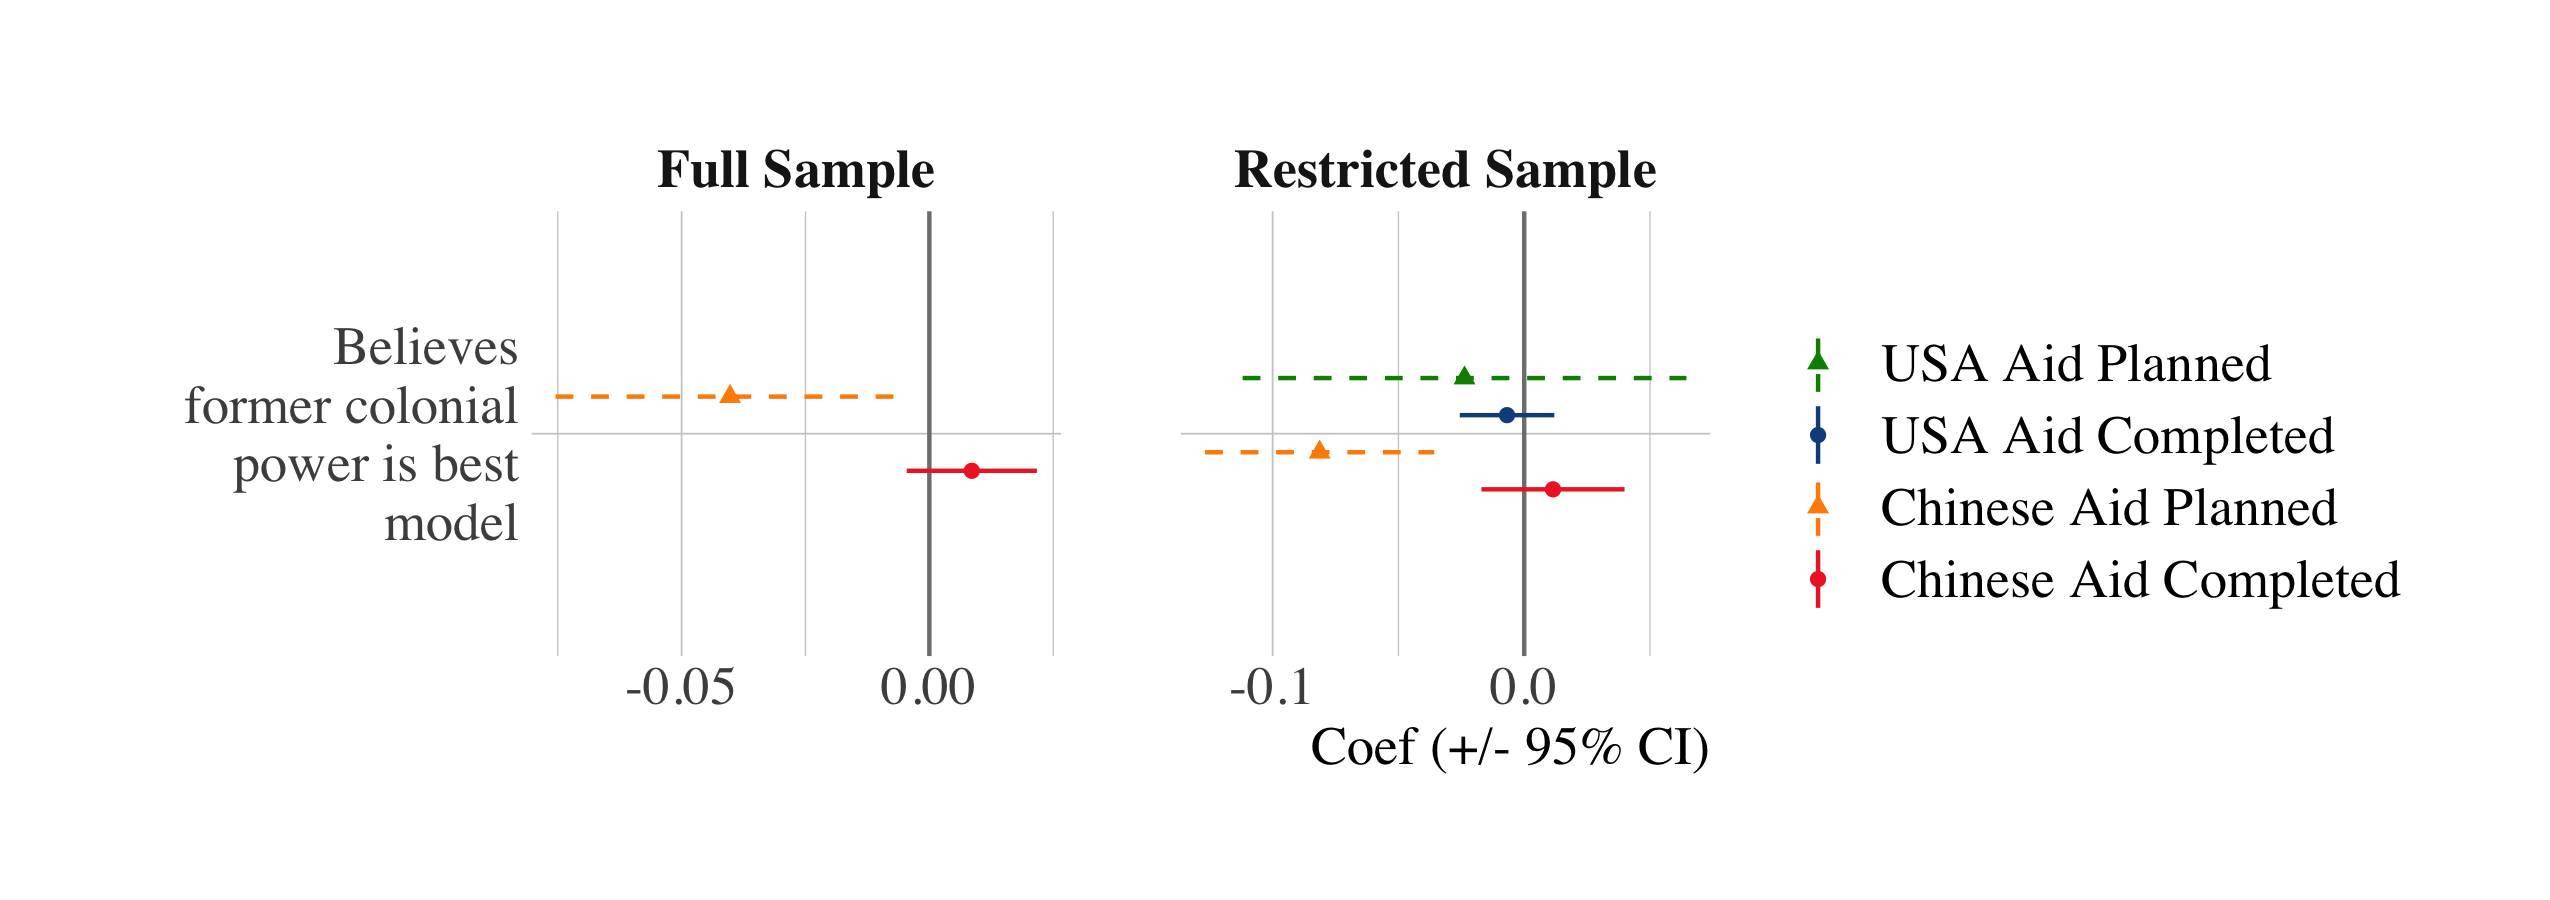
\includegraphics[width=1\textwidth]{figures/figure_a5.png}
\caption{Effects of Chinese and US aid on perceptions of former colonial powers, using 2008 as cutoff year}
\end{figure}

\begin{figure}[H]
\centering
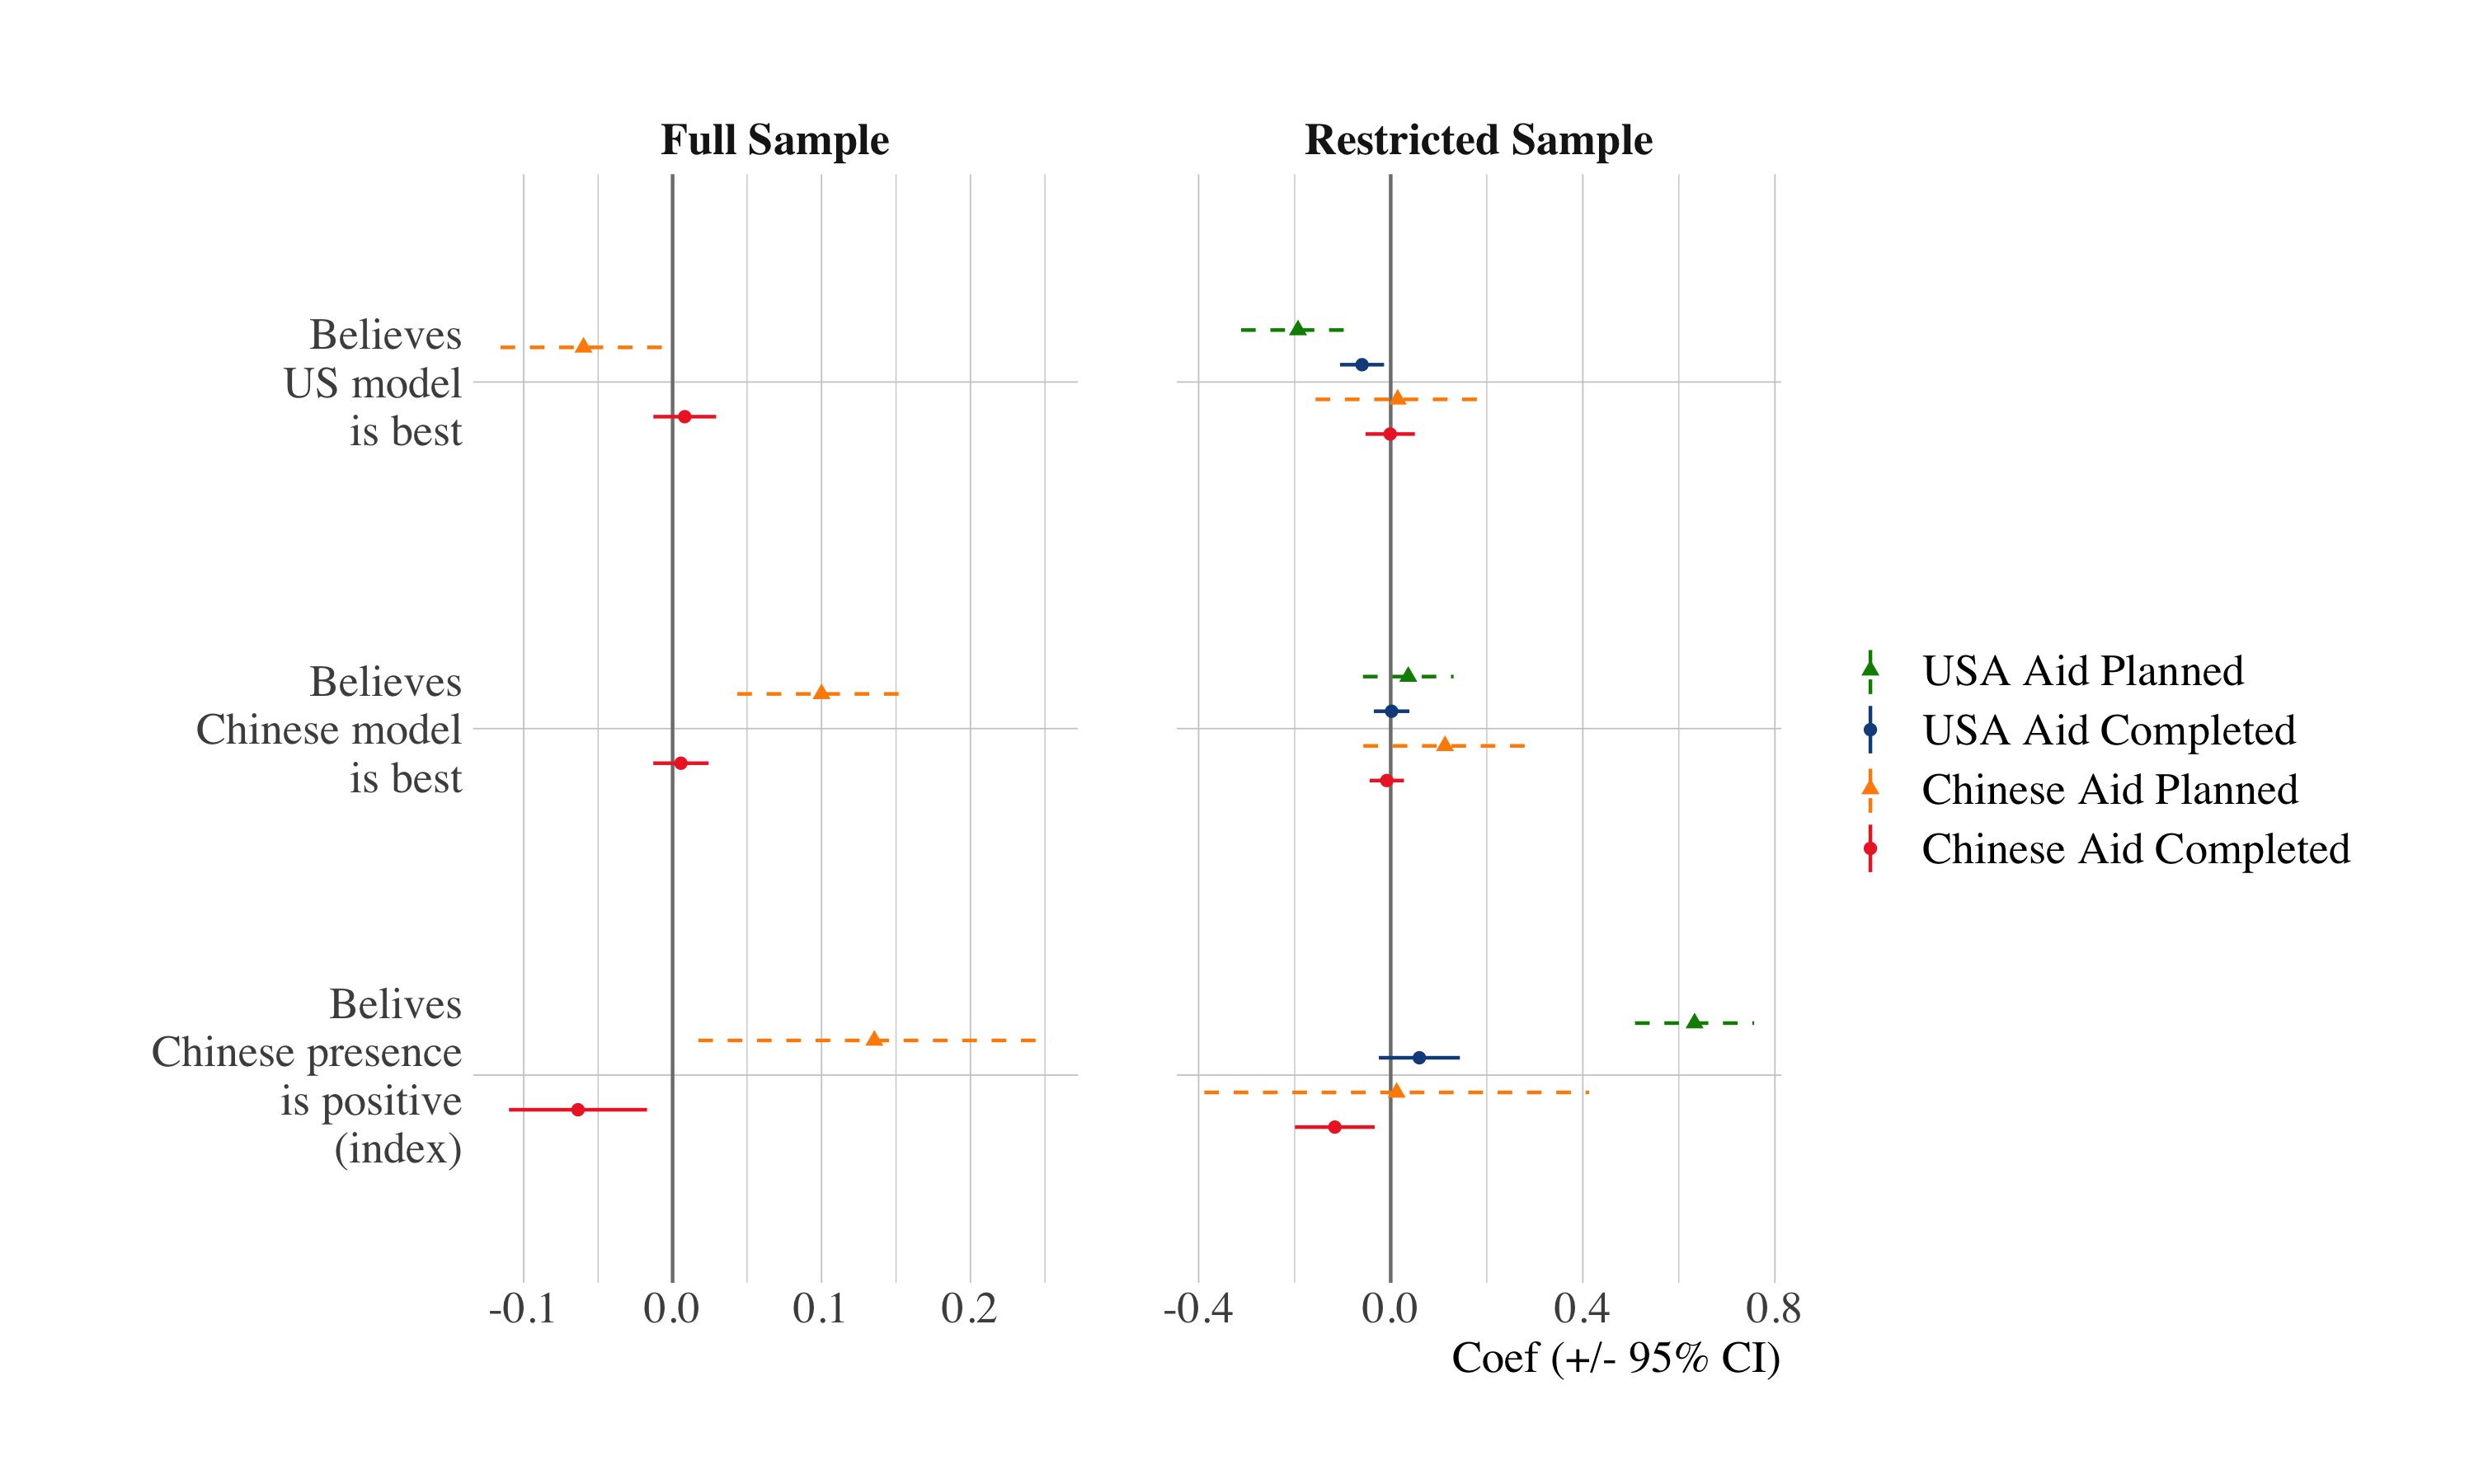
\includegraphics[width=1\textwidth]{figures/figure_a6.png}
\caption{Effects of Chinese and US aid on perceptions of China and the US, using 2009 as cutoff year}
\end{figure}

\begin{figure}[H]
\centering
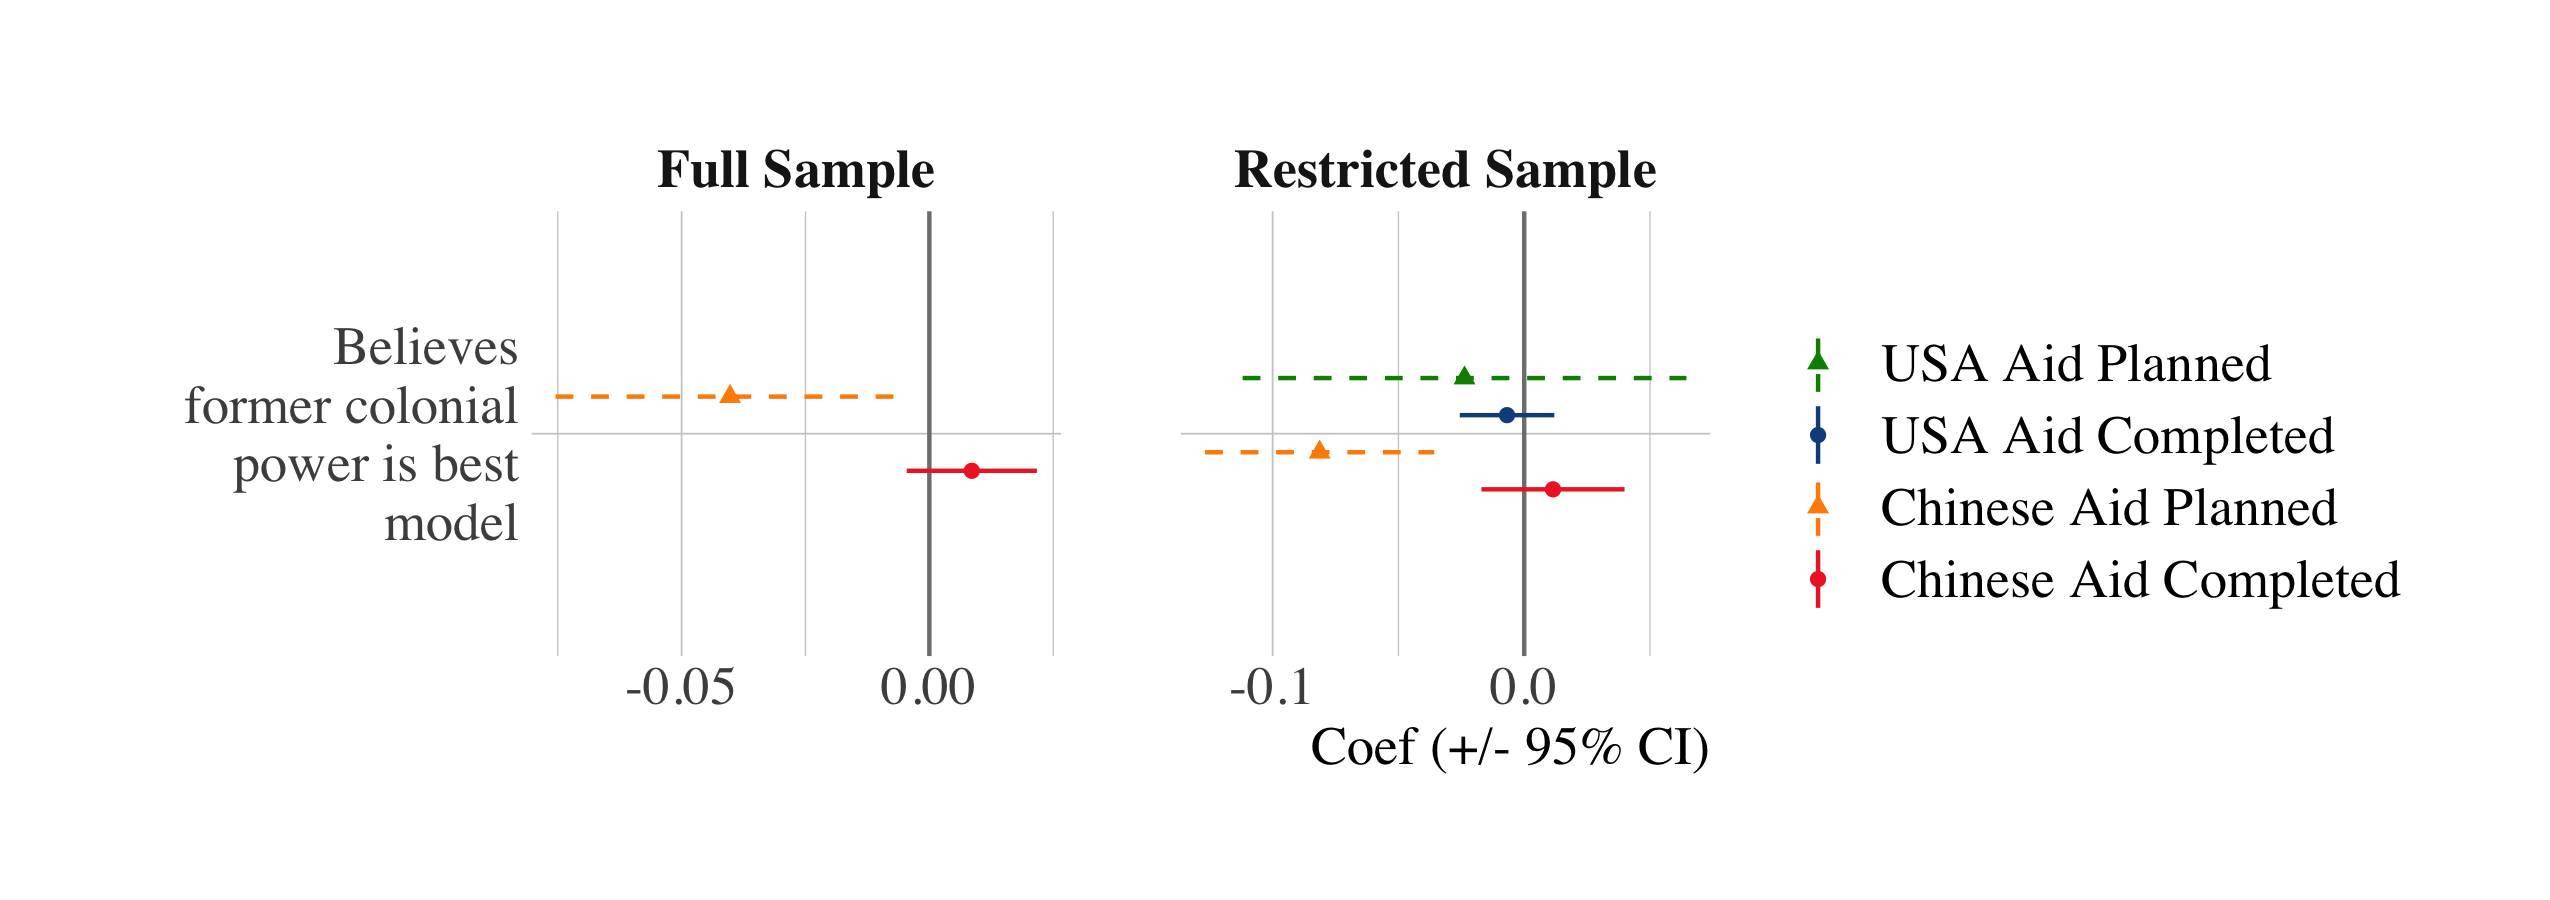
\includegraphics[width=1\textwidth]{figures/figure_a7.png}
\caption{Effects of Chinese and US aid on perceptions of former colonial powers, using 2009 as cutoff year}
\end{figure}

\begin{figure}[H]
\centering
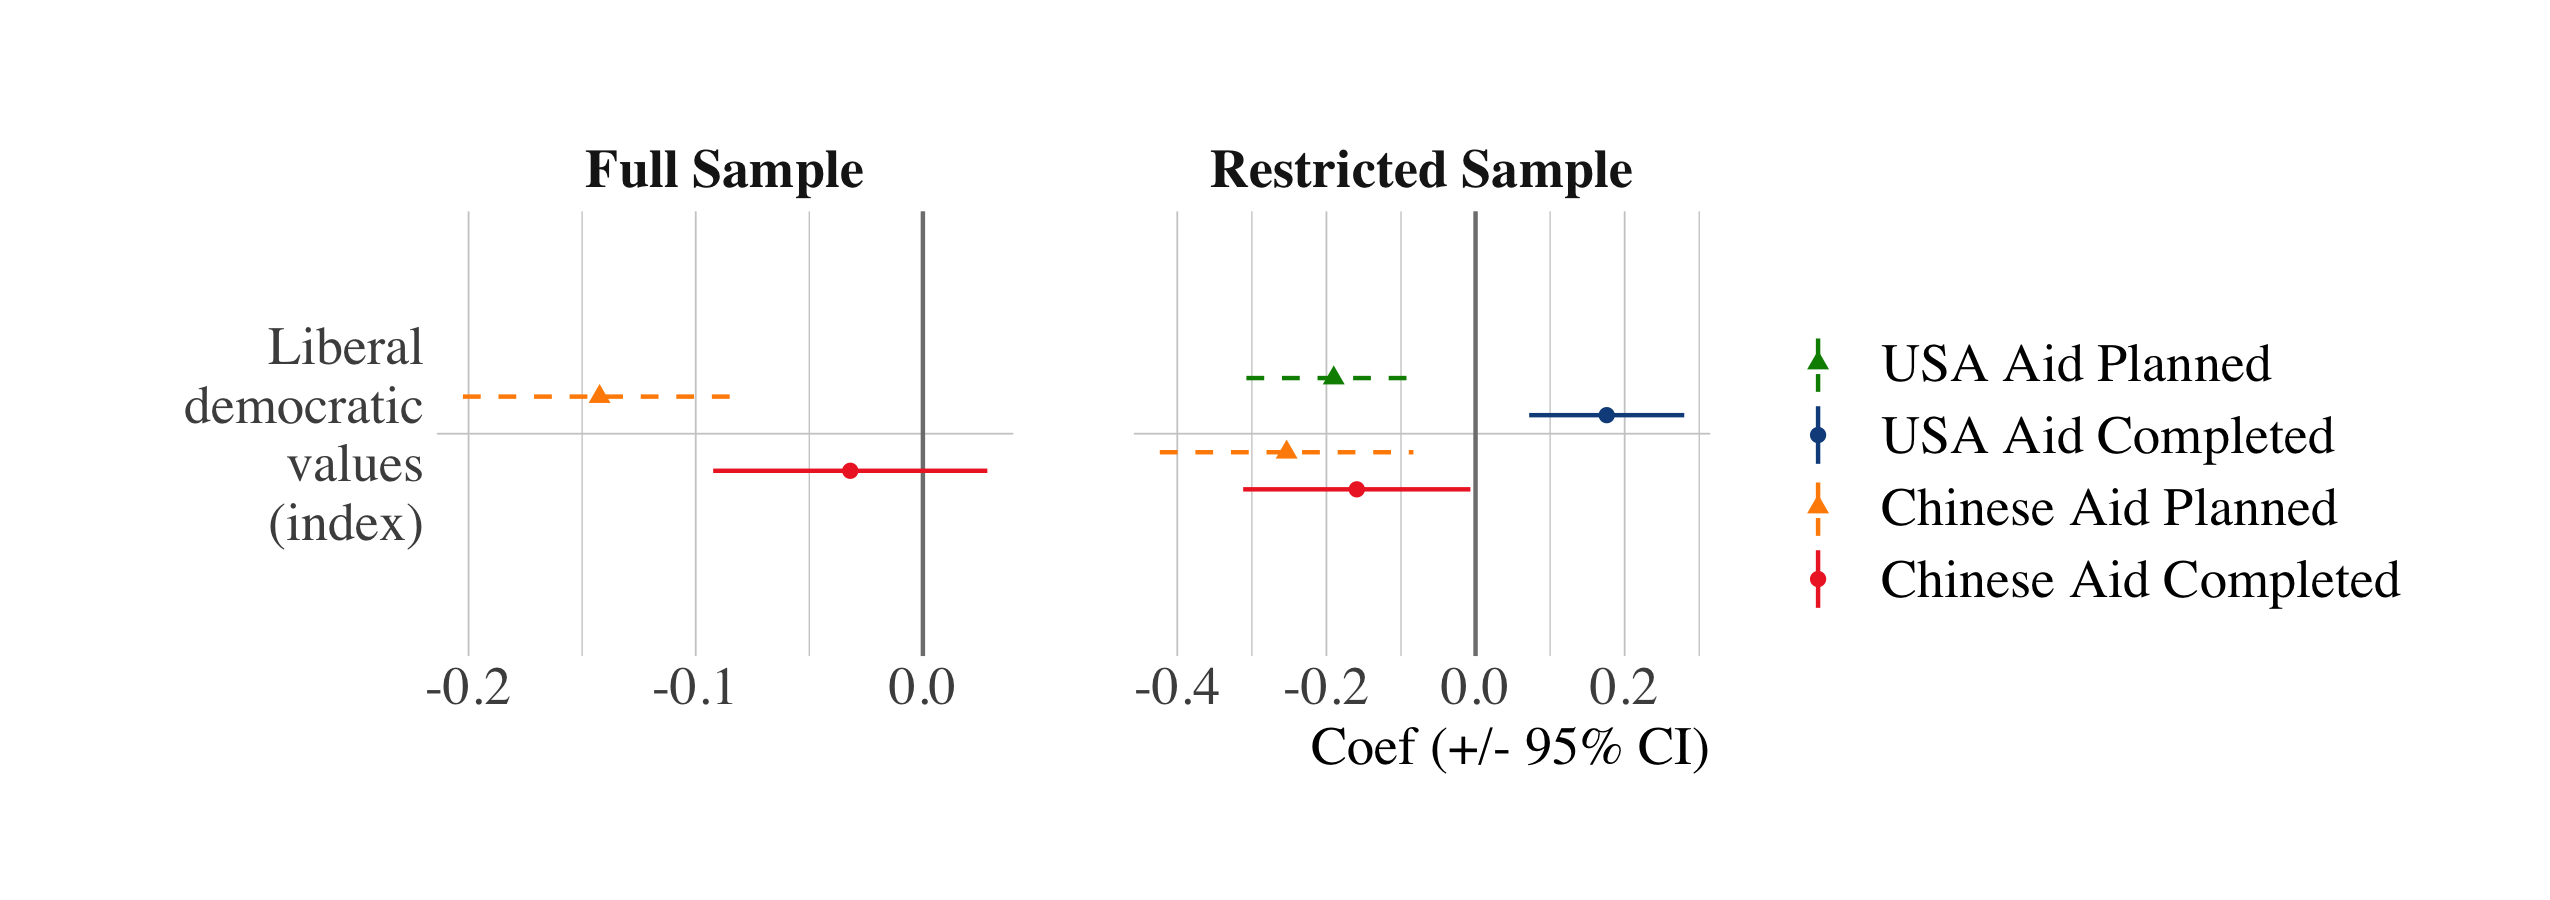
\includegraphics[width=1\textwidth]{figures/figure_a8.png}
\caption{Effects of Chinese and US aid on liberal democratic values, using only planned projects that we know were completed}
\end{figure}

\begin{figure}[H]
\centering
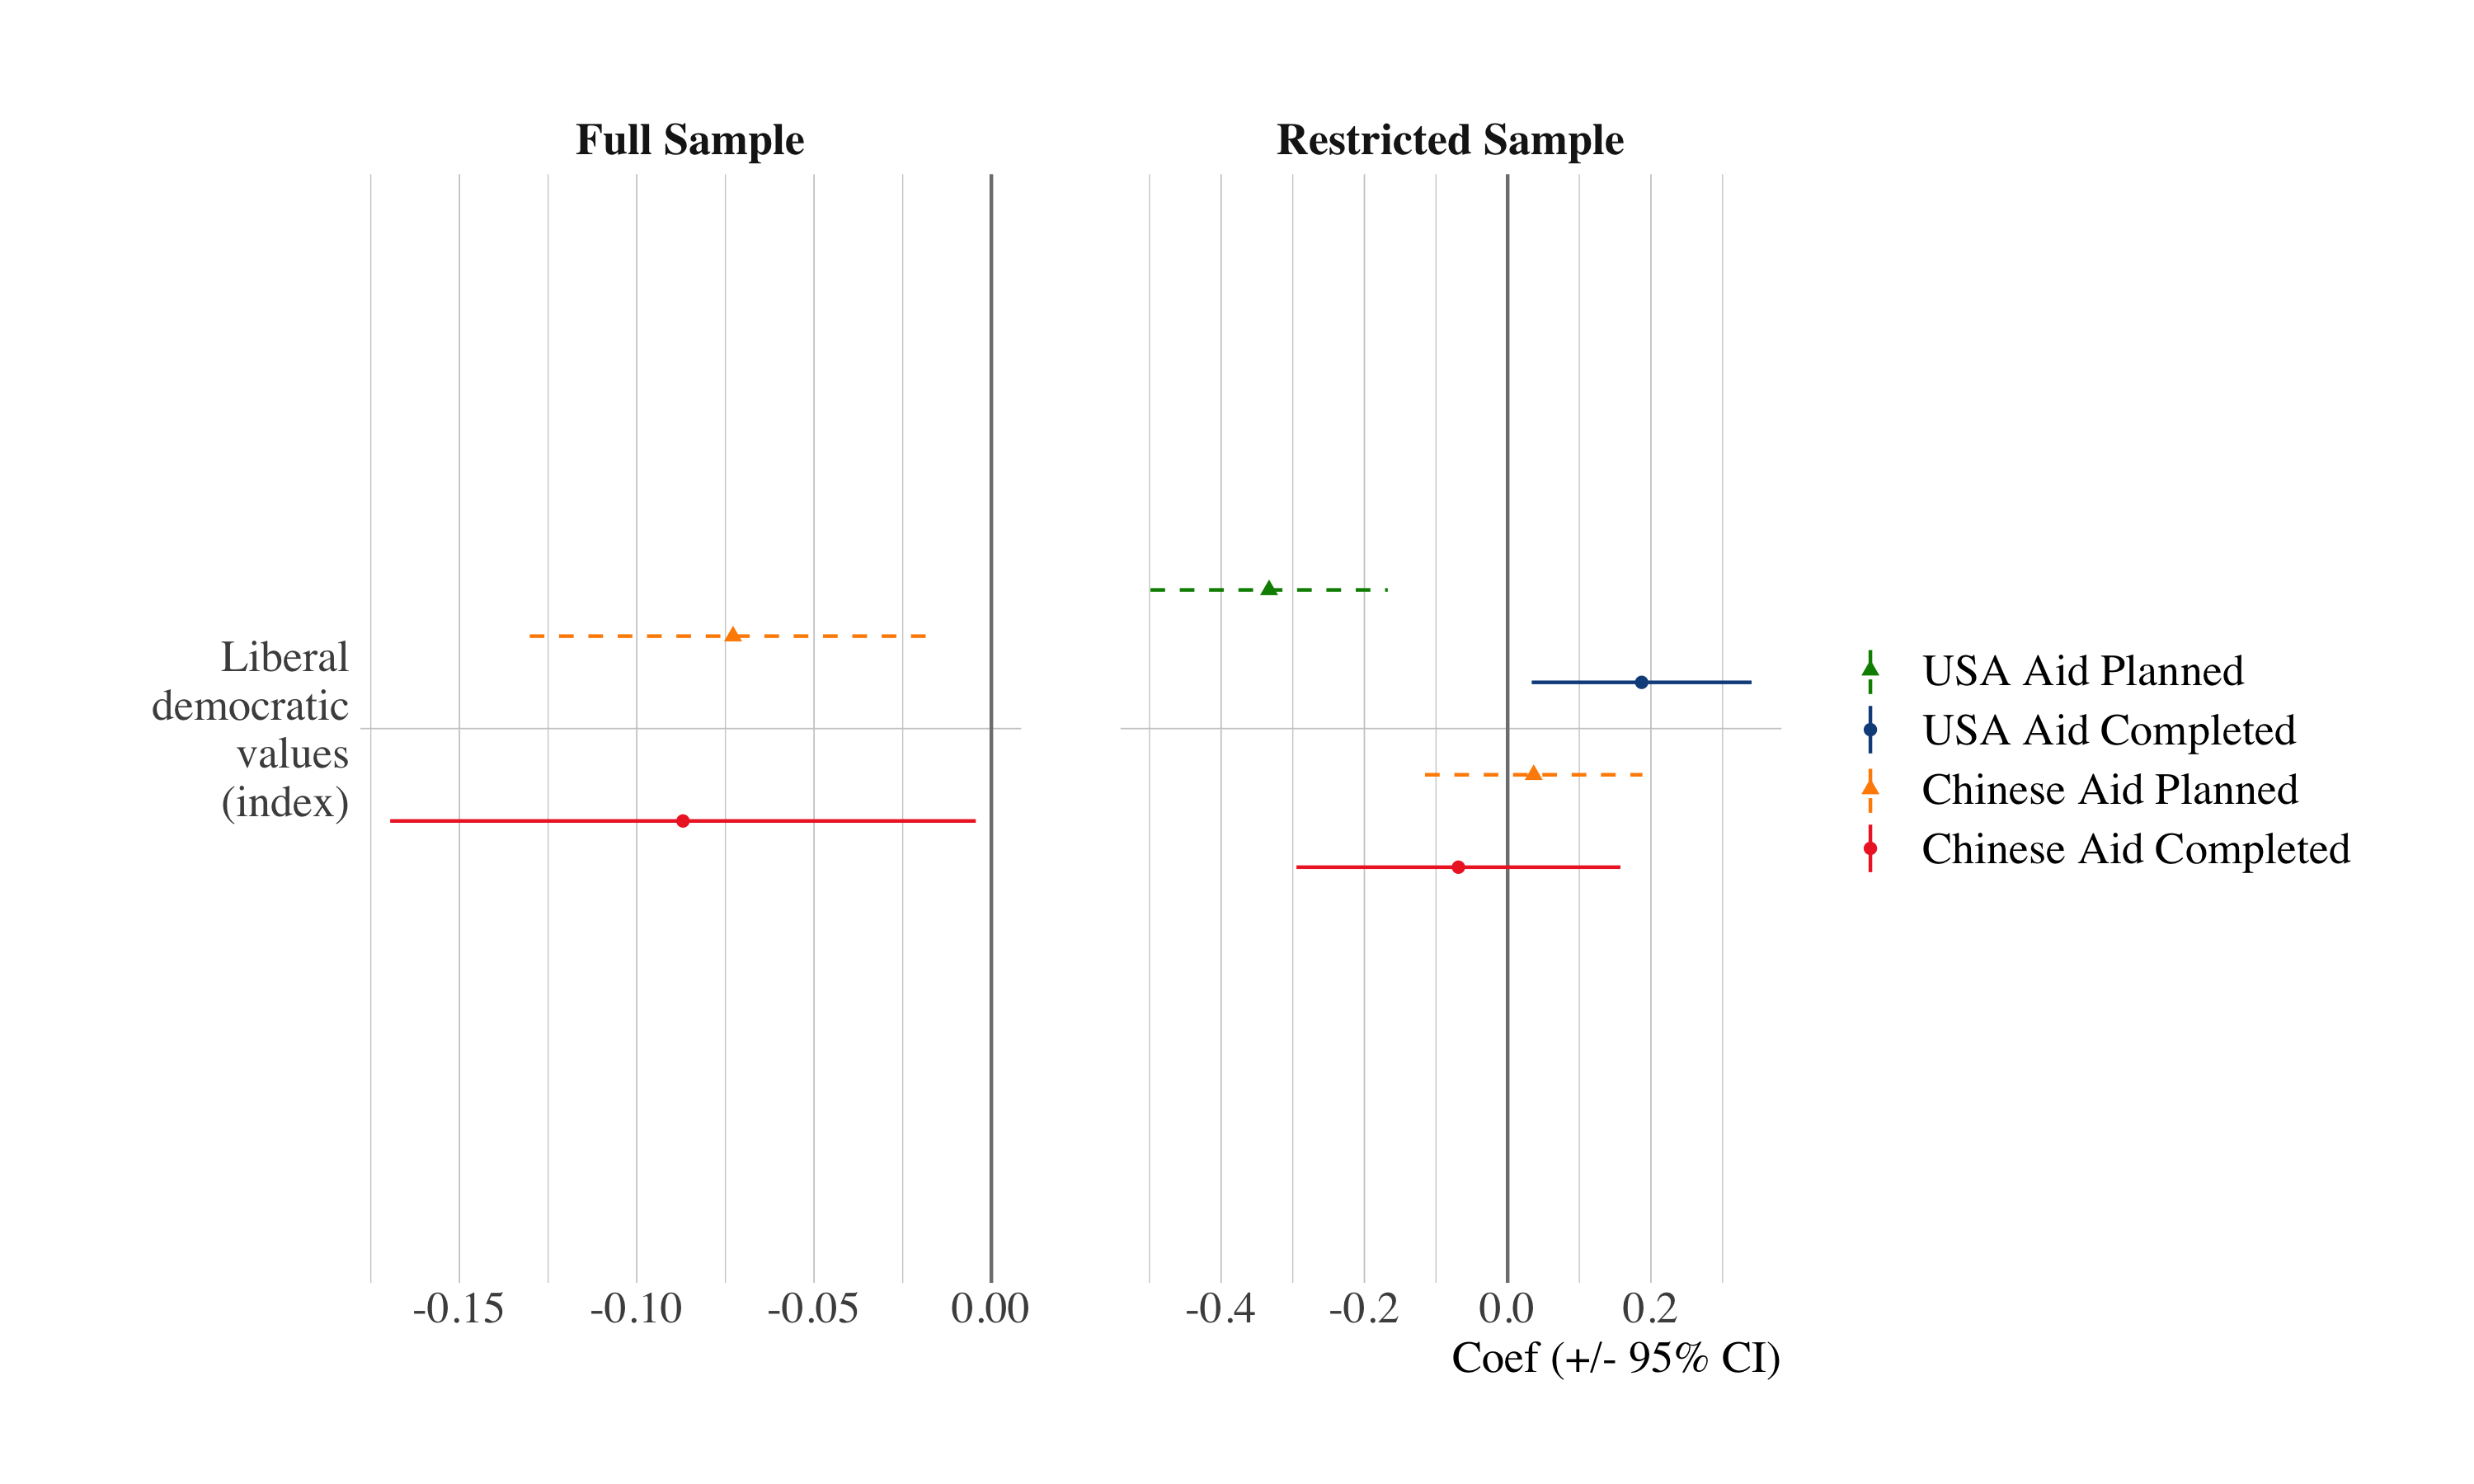
\includegraphics[width=1\textwidth]{figures/figure_a9.png}
\caption{Effects of Chinese and US aid on liberal democratic values, using first administrative level as fixed effect}
\end{figure}

\begin{figure}[H]
\centering
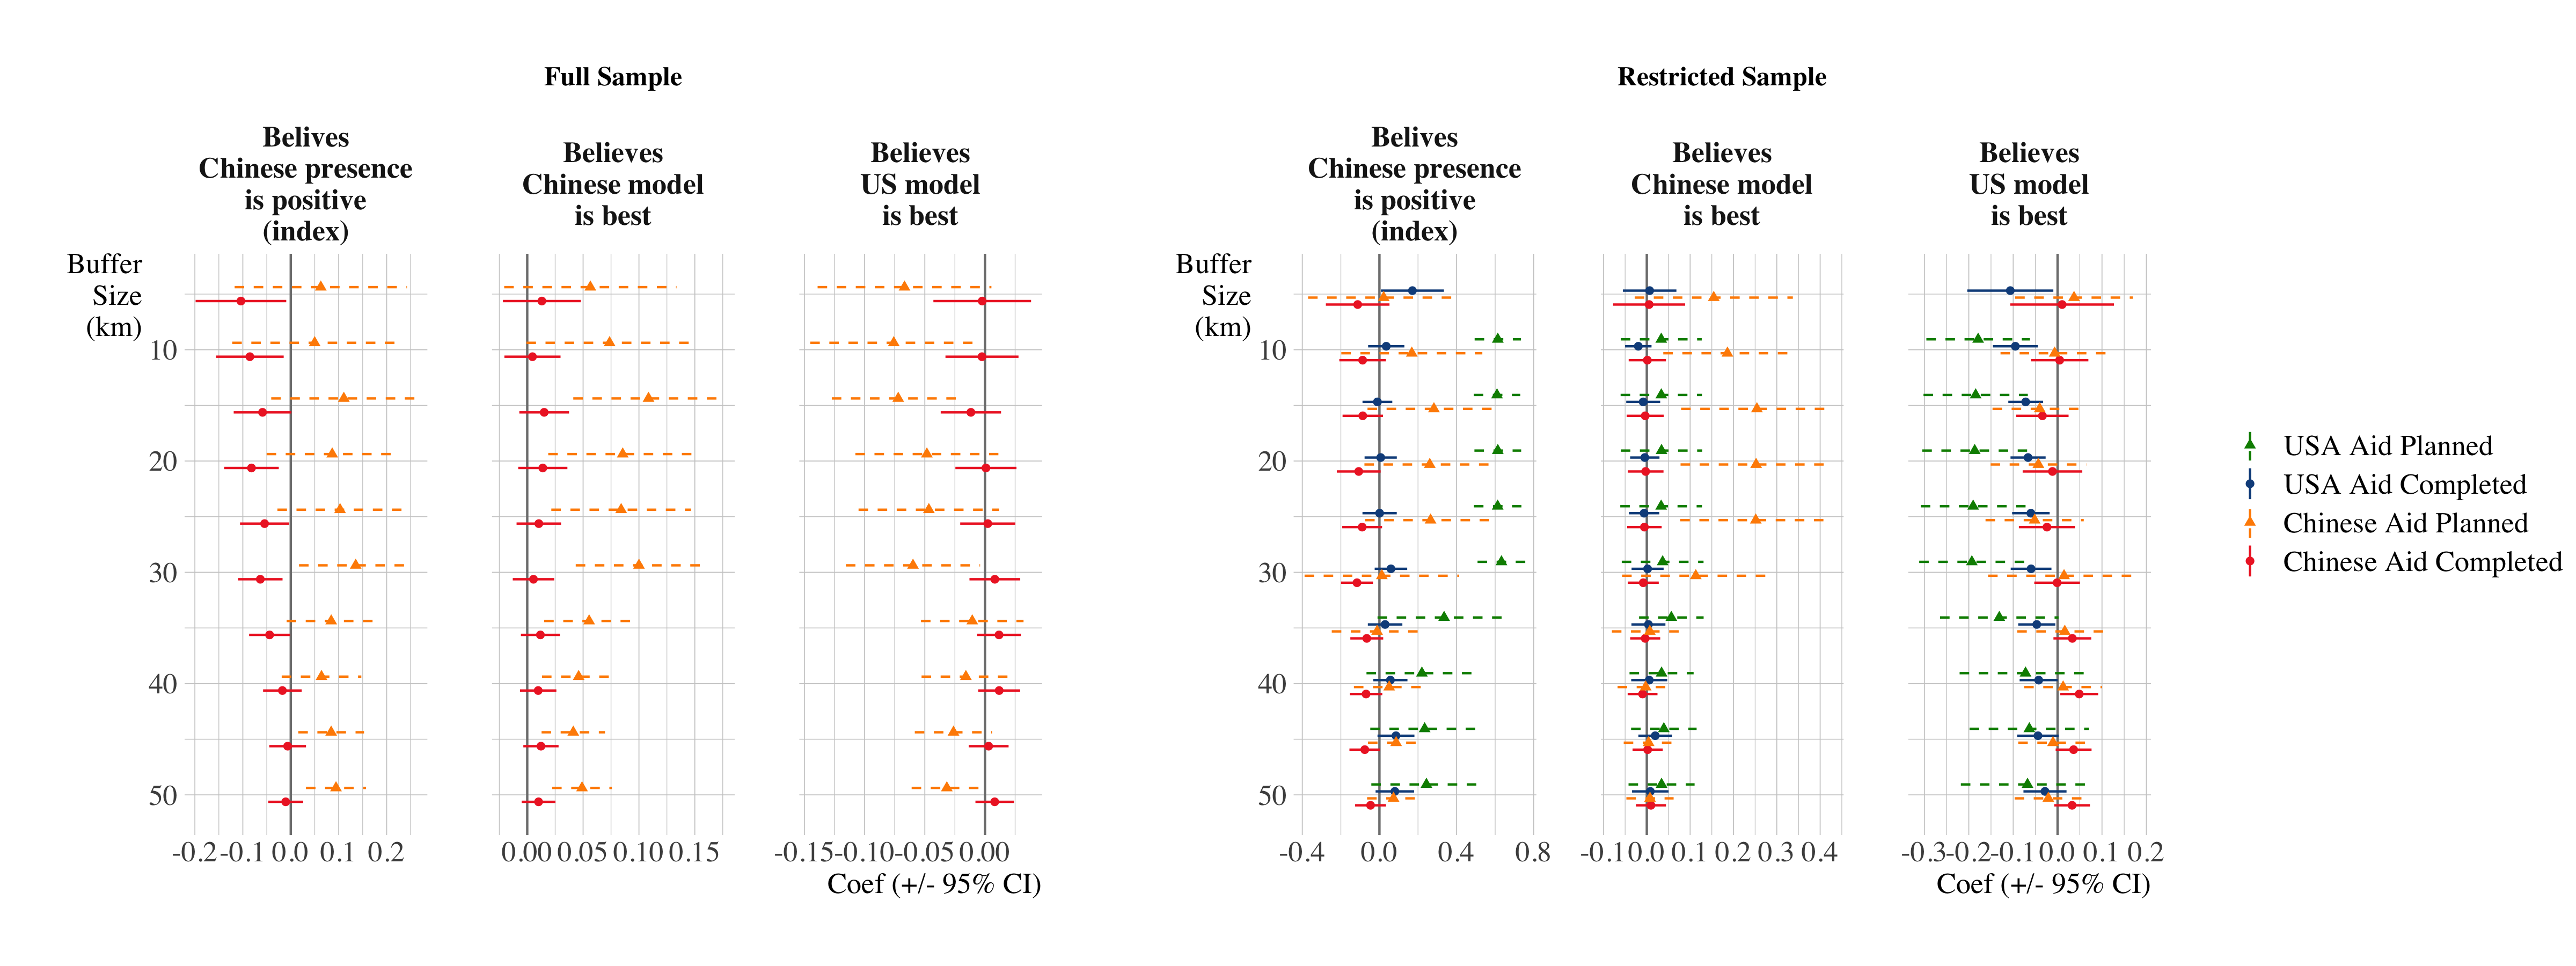
\includegraphics[width=1\textwidth]{figures/figure_a10.png}
\caption{Effects of Chinese and US aid on perceptions of China and the US, varying buffer}
\end{figure}

\begin{figure}[H]
\centering
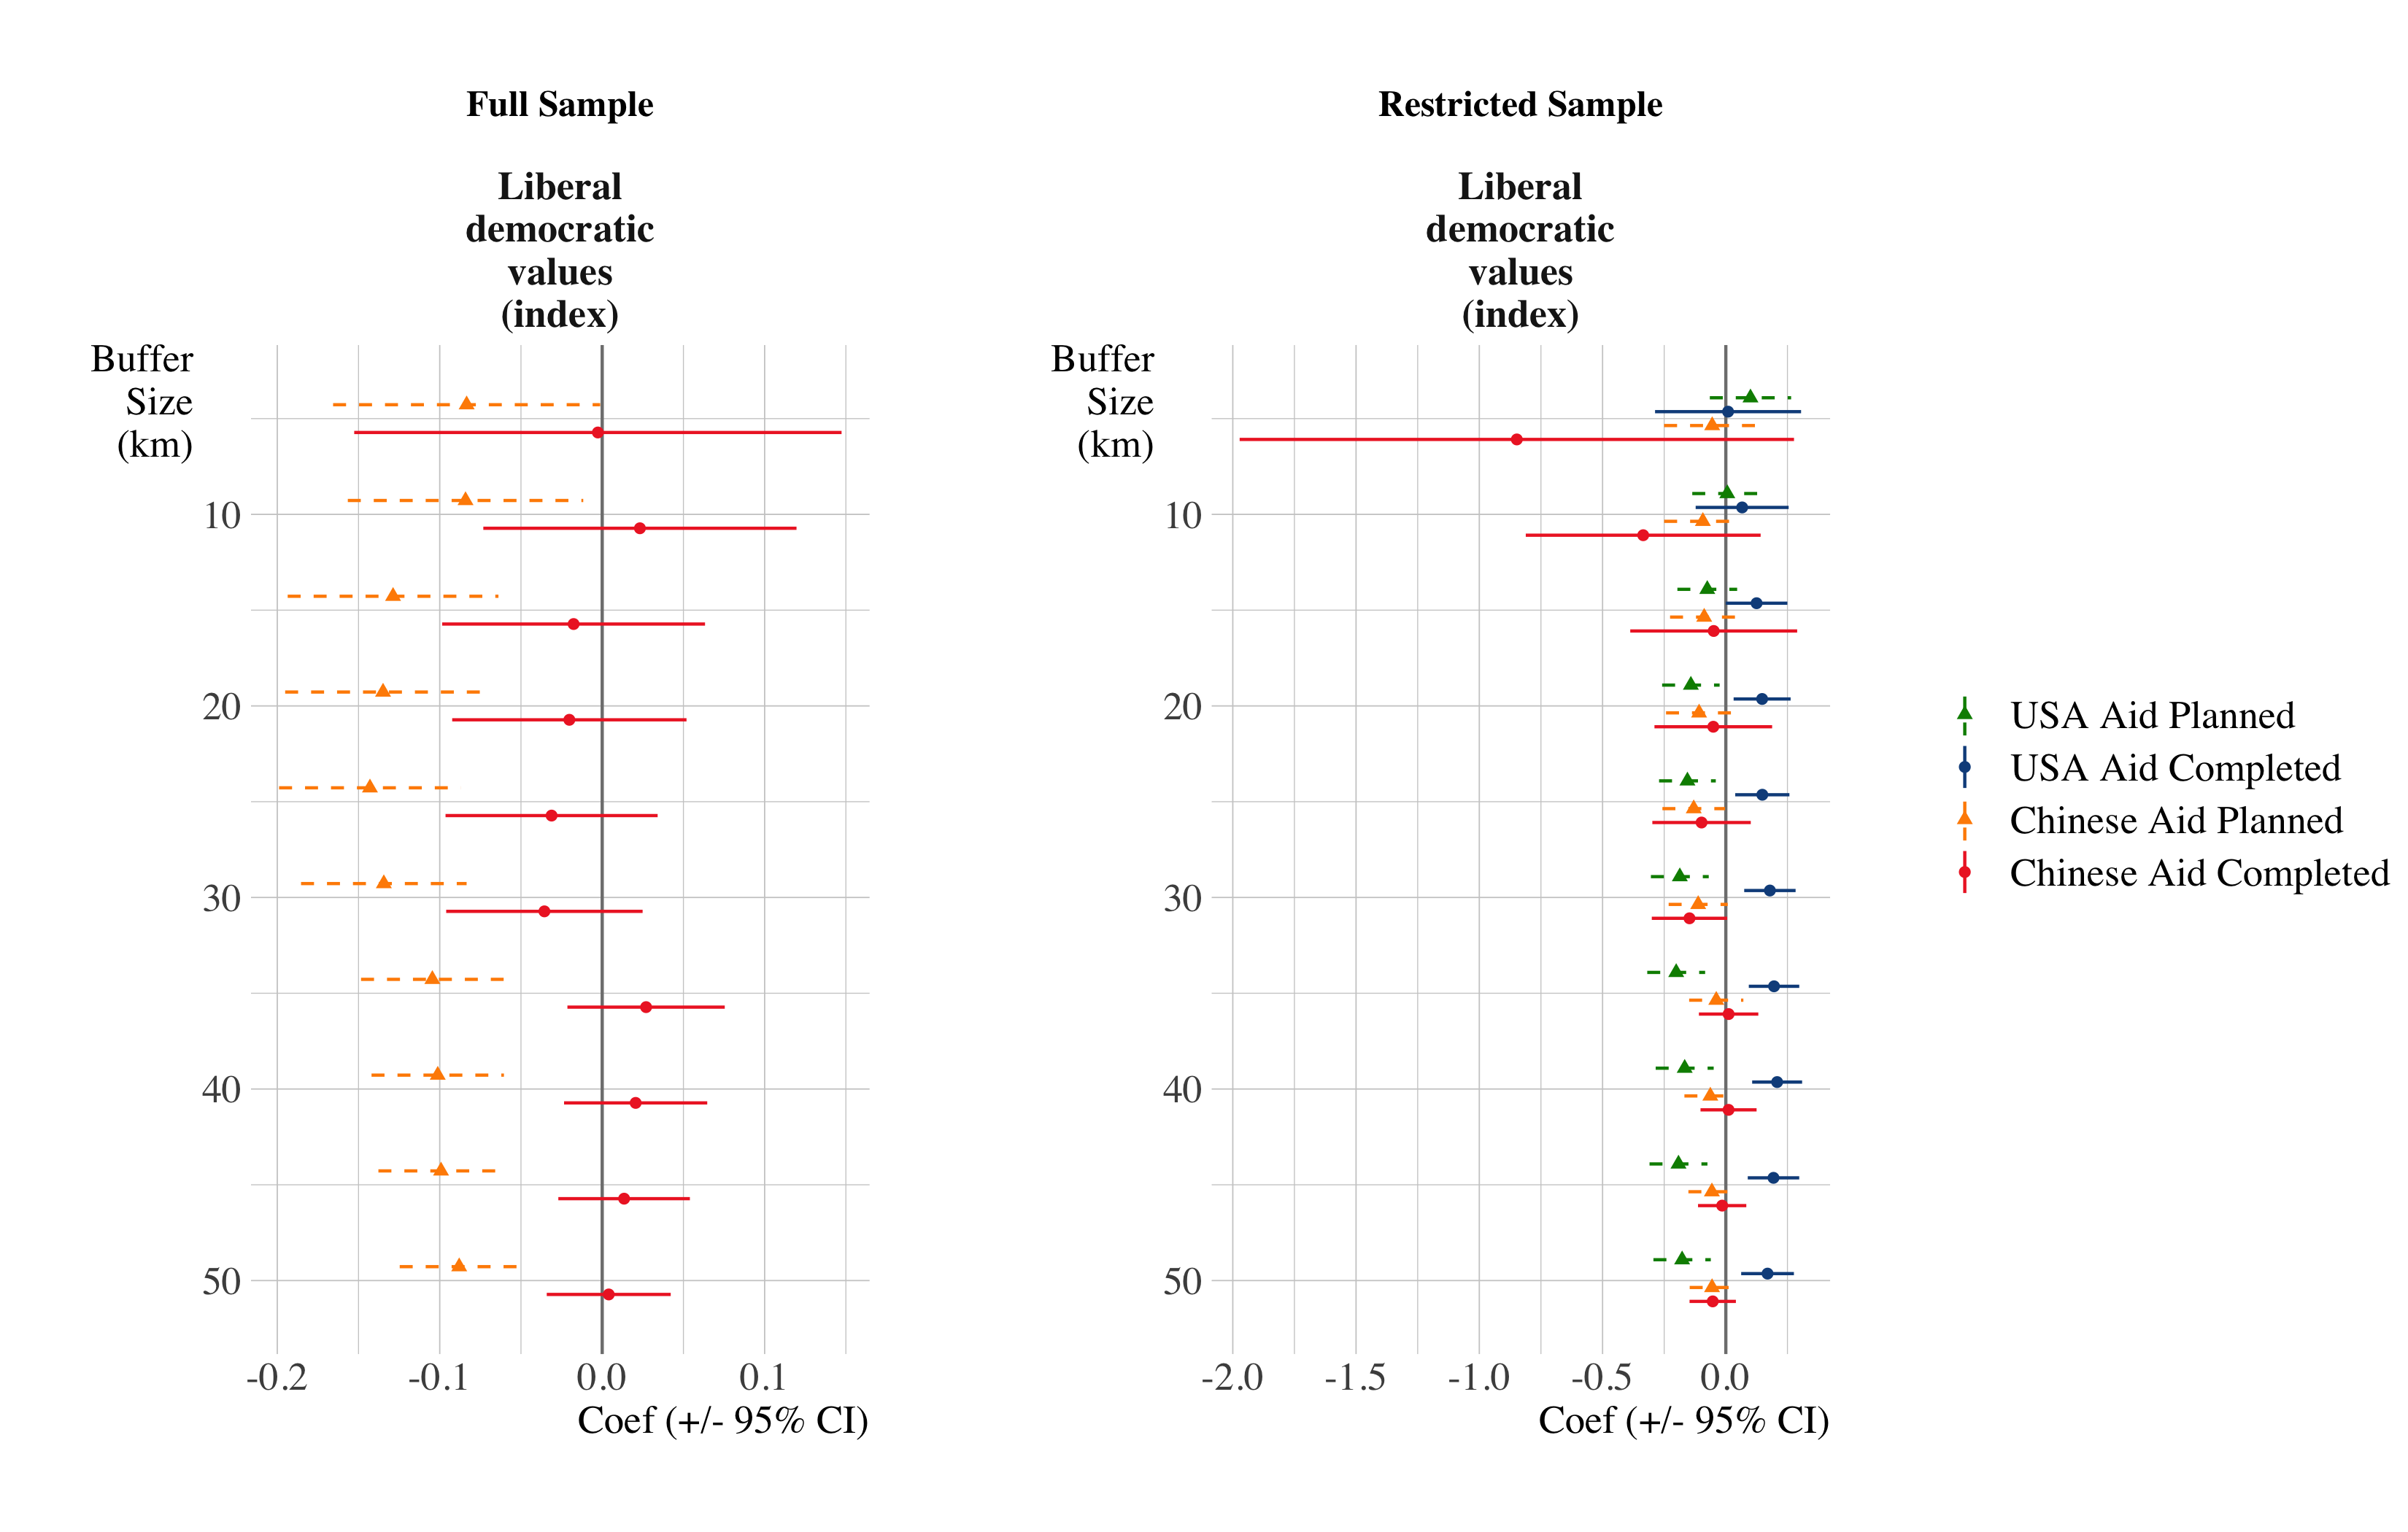
\includegraphics[width=0.8\textwidth]{figures/figure_a11.png}
\caption{Effects of Chinese and US aid on liberal democratic values, varying buffer}
\end{figure}

\begin{figure}[H]
\centering
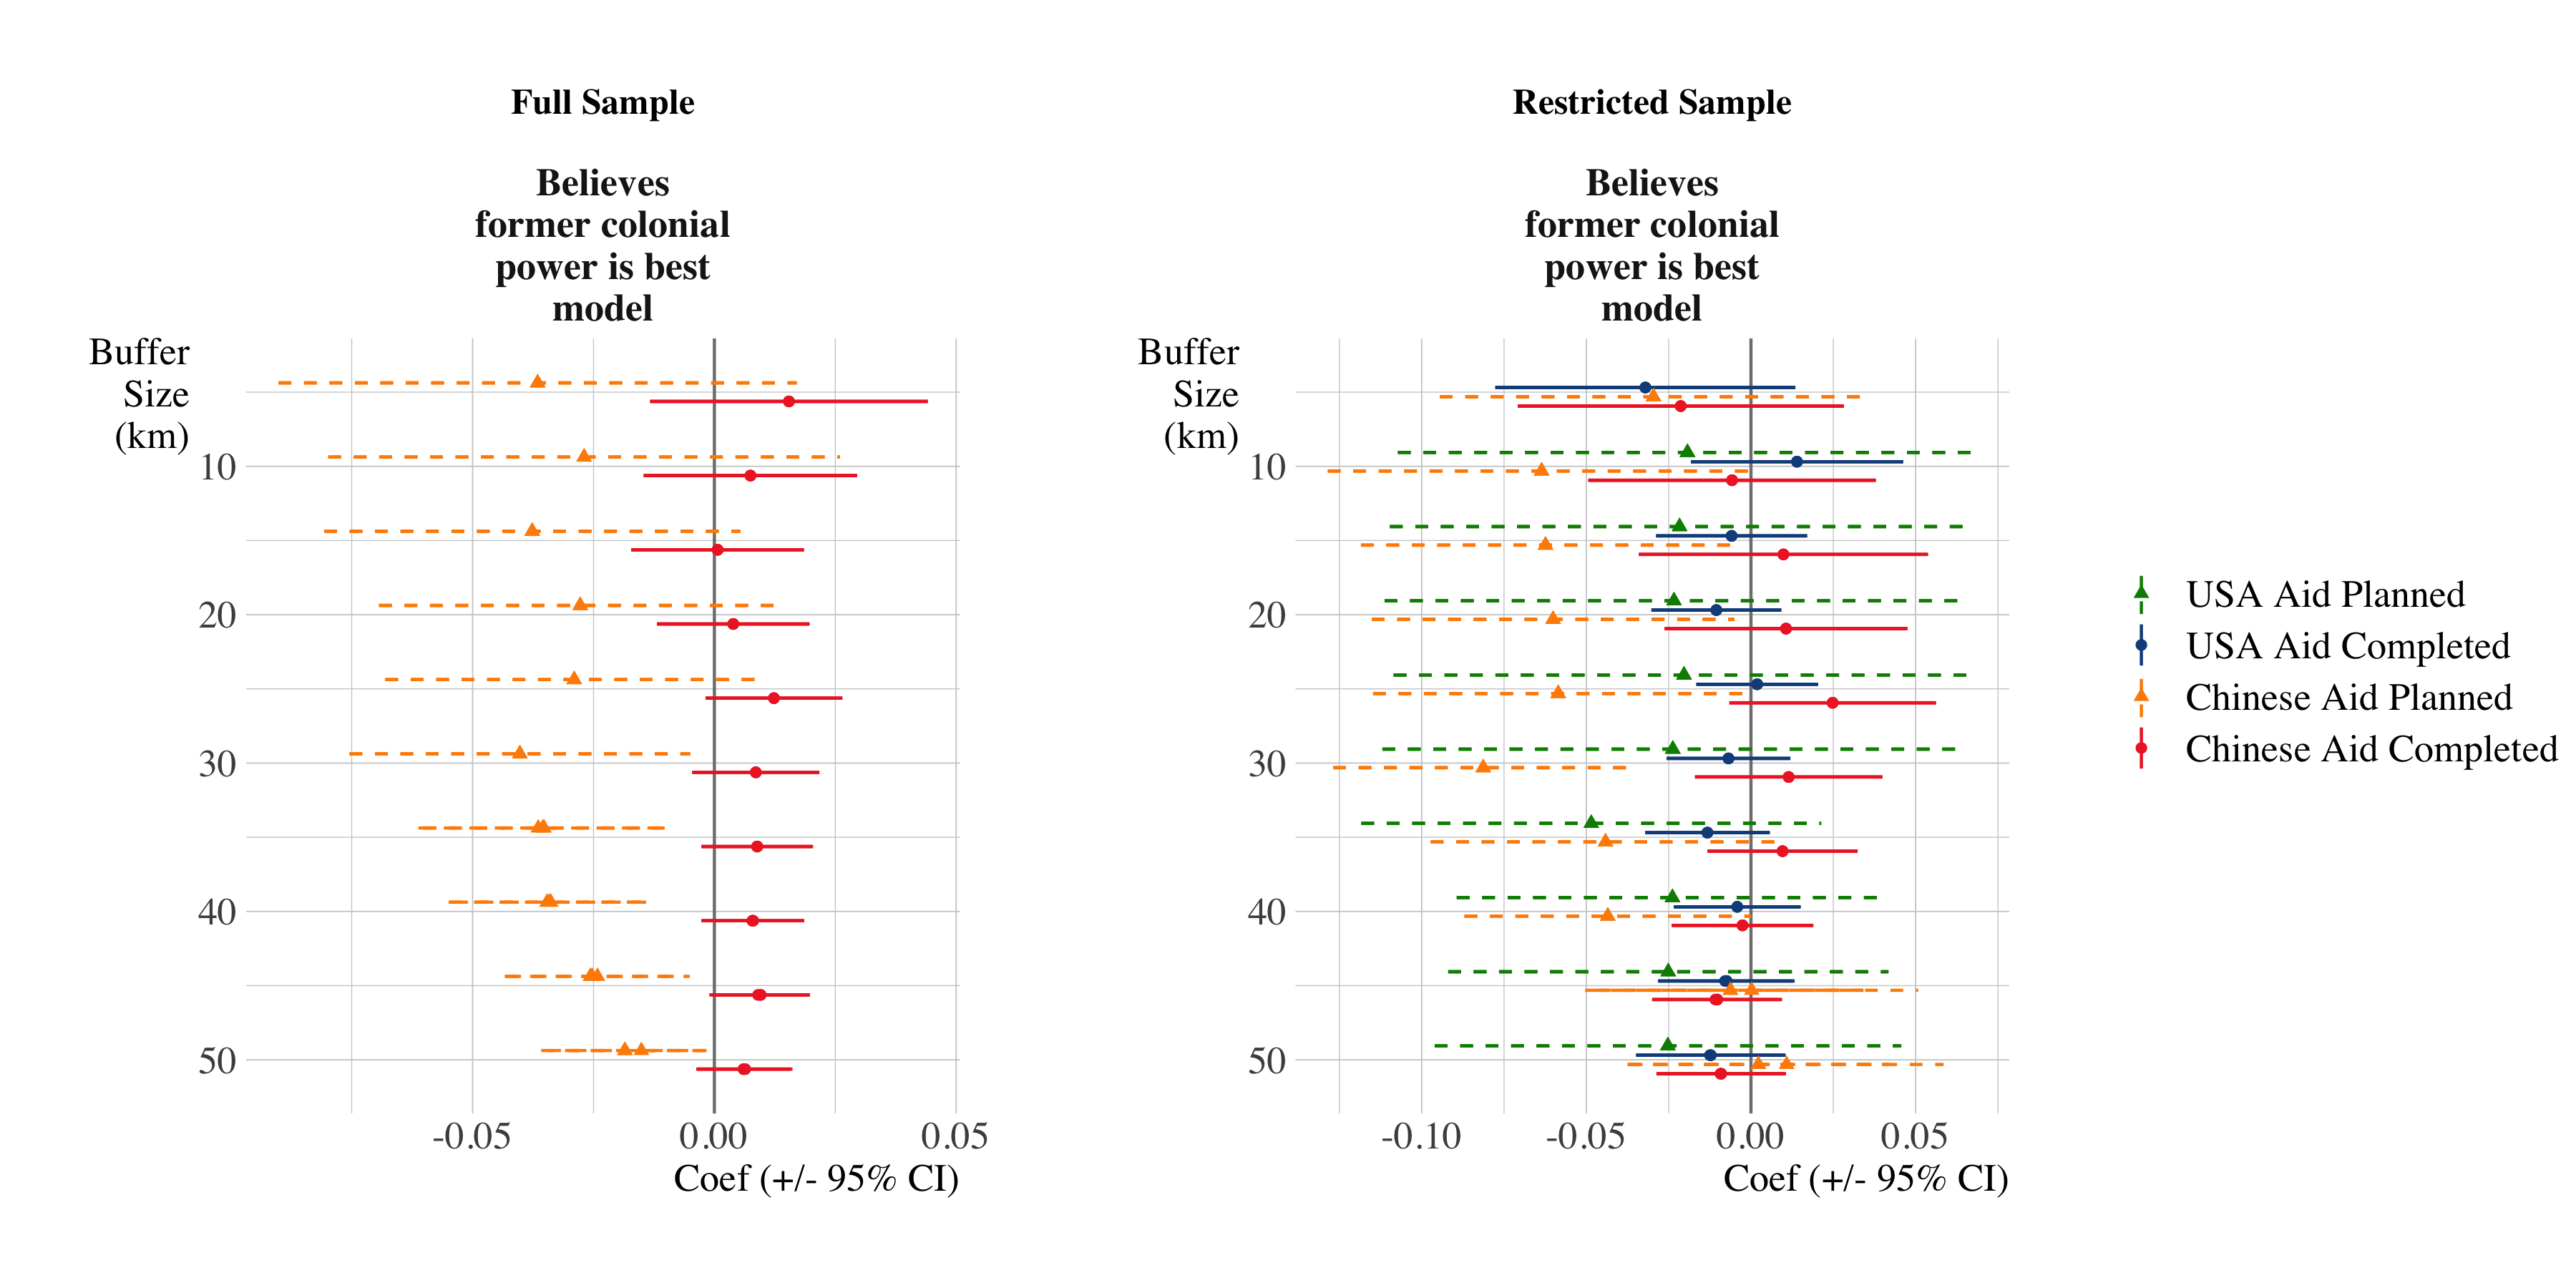
\includegraphics[width=0.8\textwidth]{figures/figure_a12.png}
\caption{Effects of Chinese and US aid on perceptions of former colonial powers, varying buffer}
\end{figure}

\begin{figure}[H]
\centering
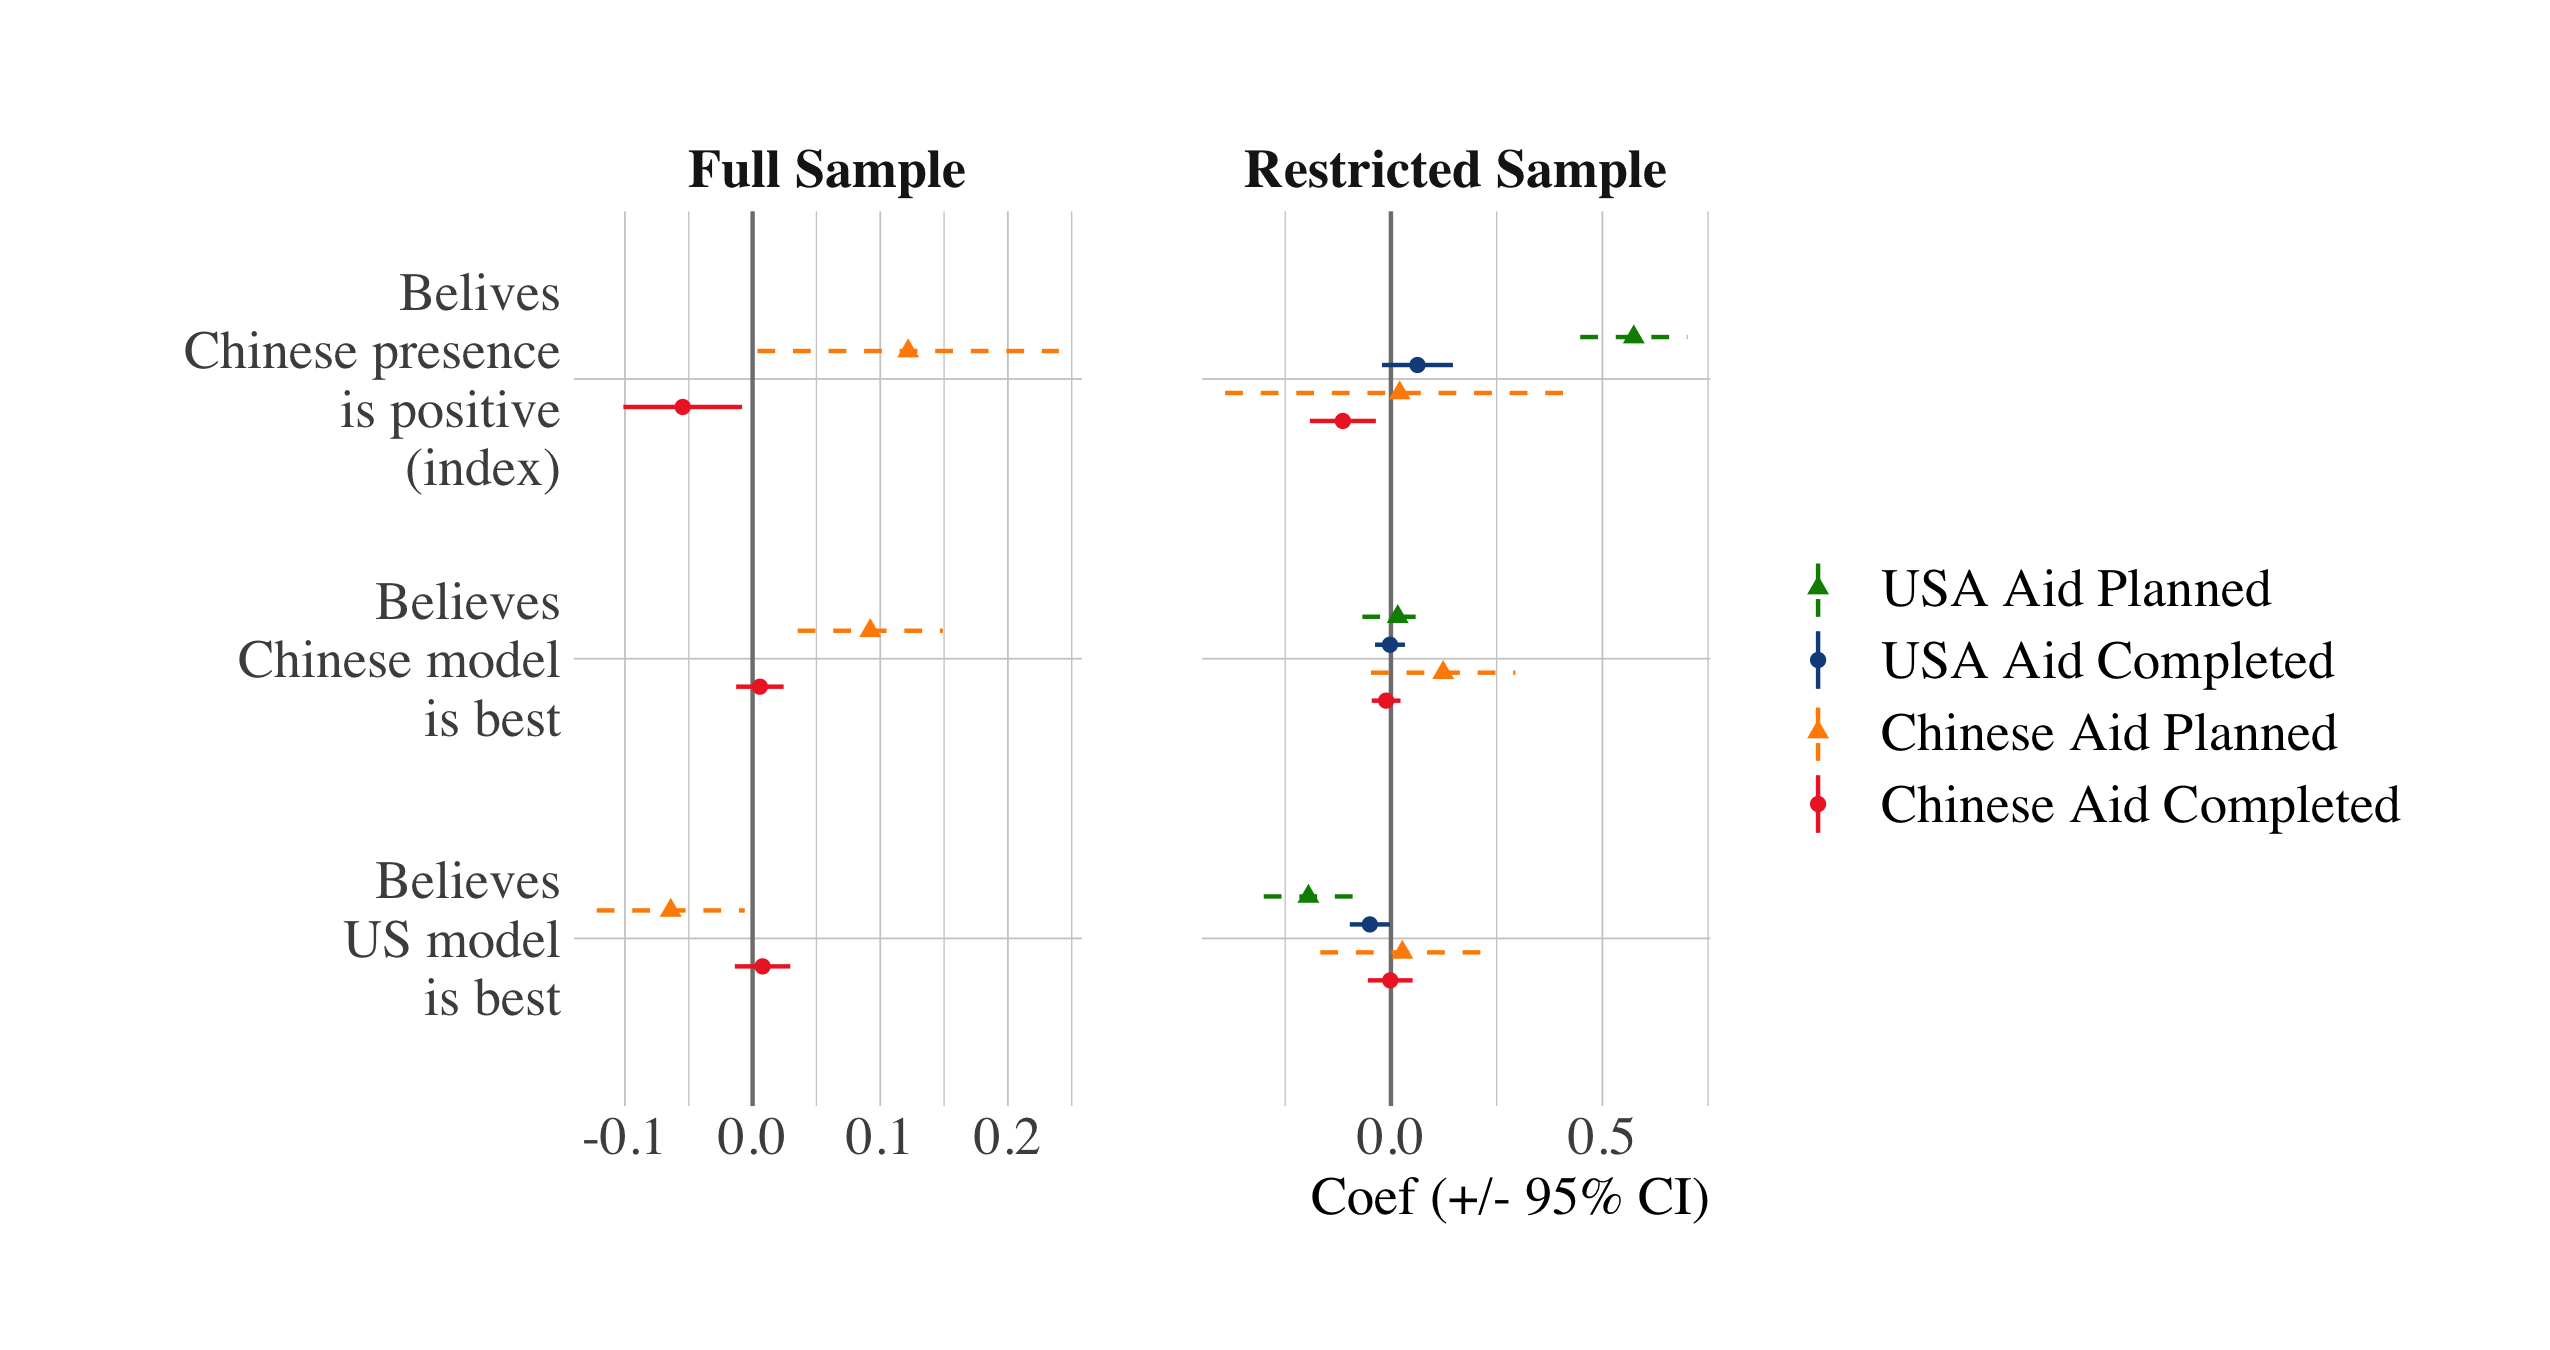
\includegraphics[width=1\textwidth]{figures/figure_a13.png}
\caption{Effects of Chinese and US aid on perceptions of China and the US, including additional controls}
\end{figure}

\begin{figure}[H]
\centering
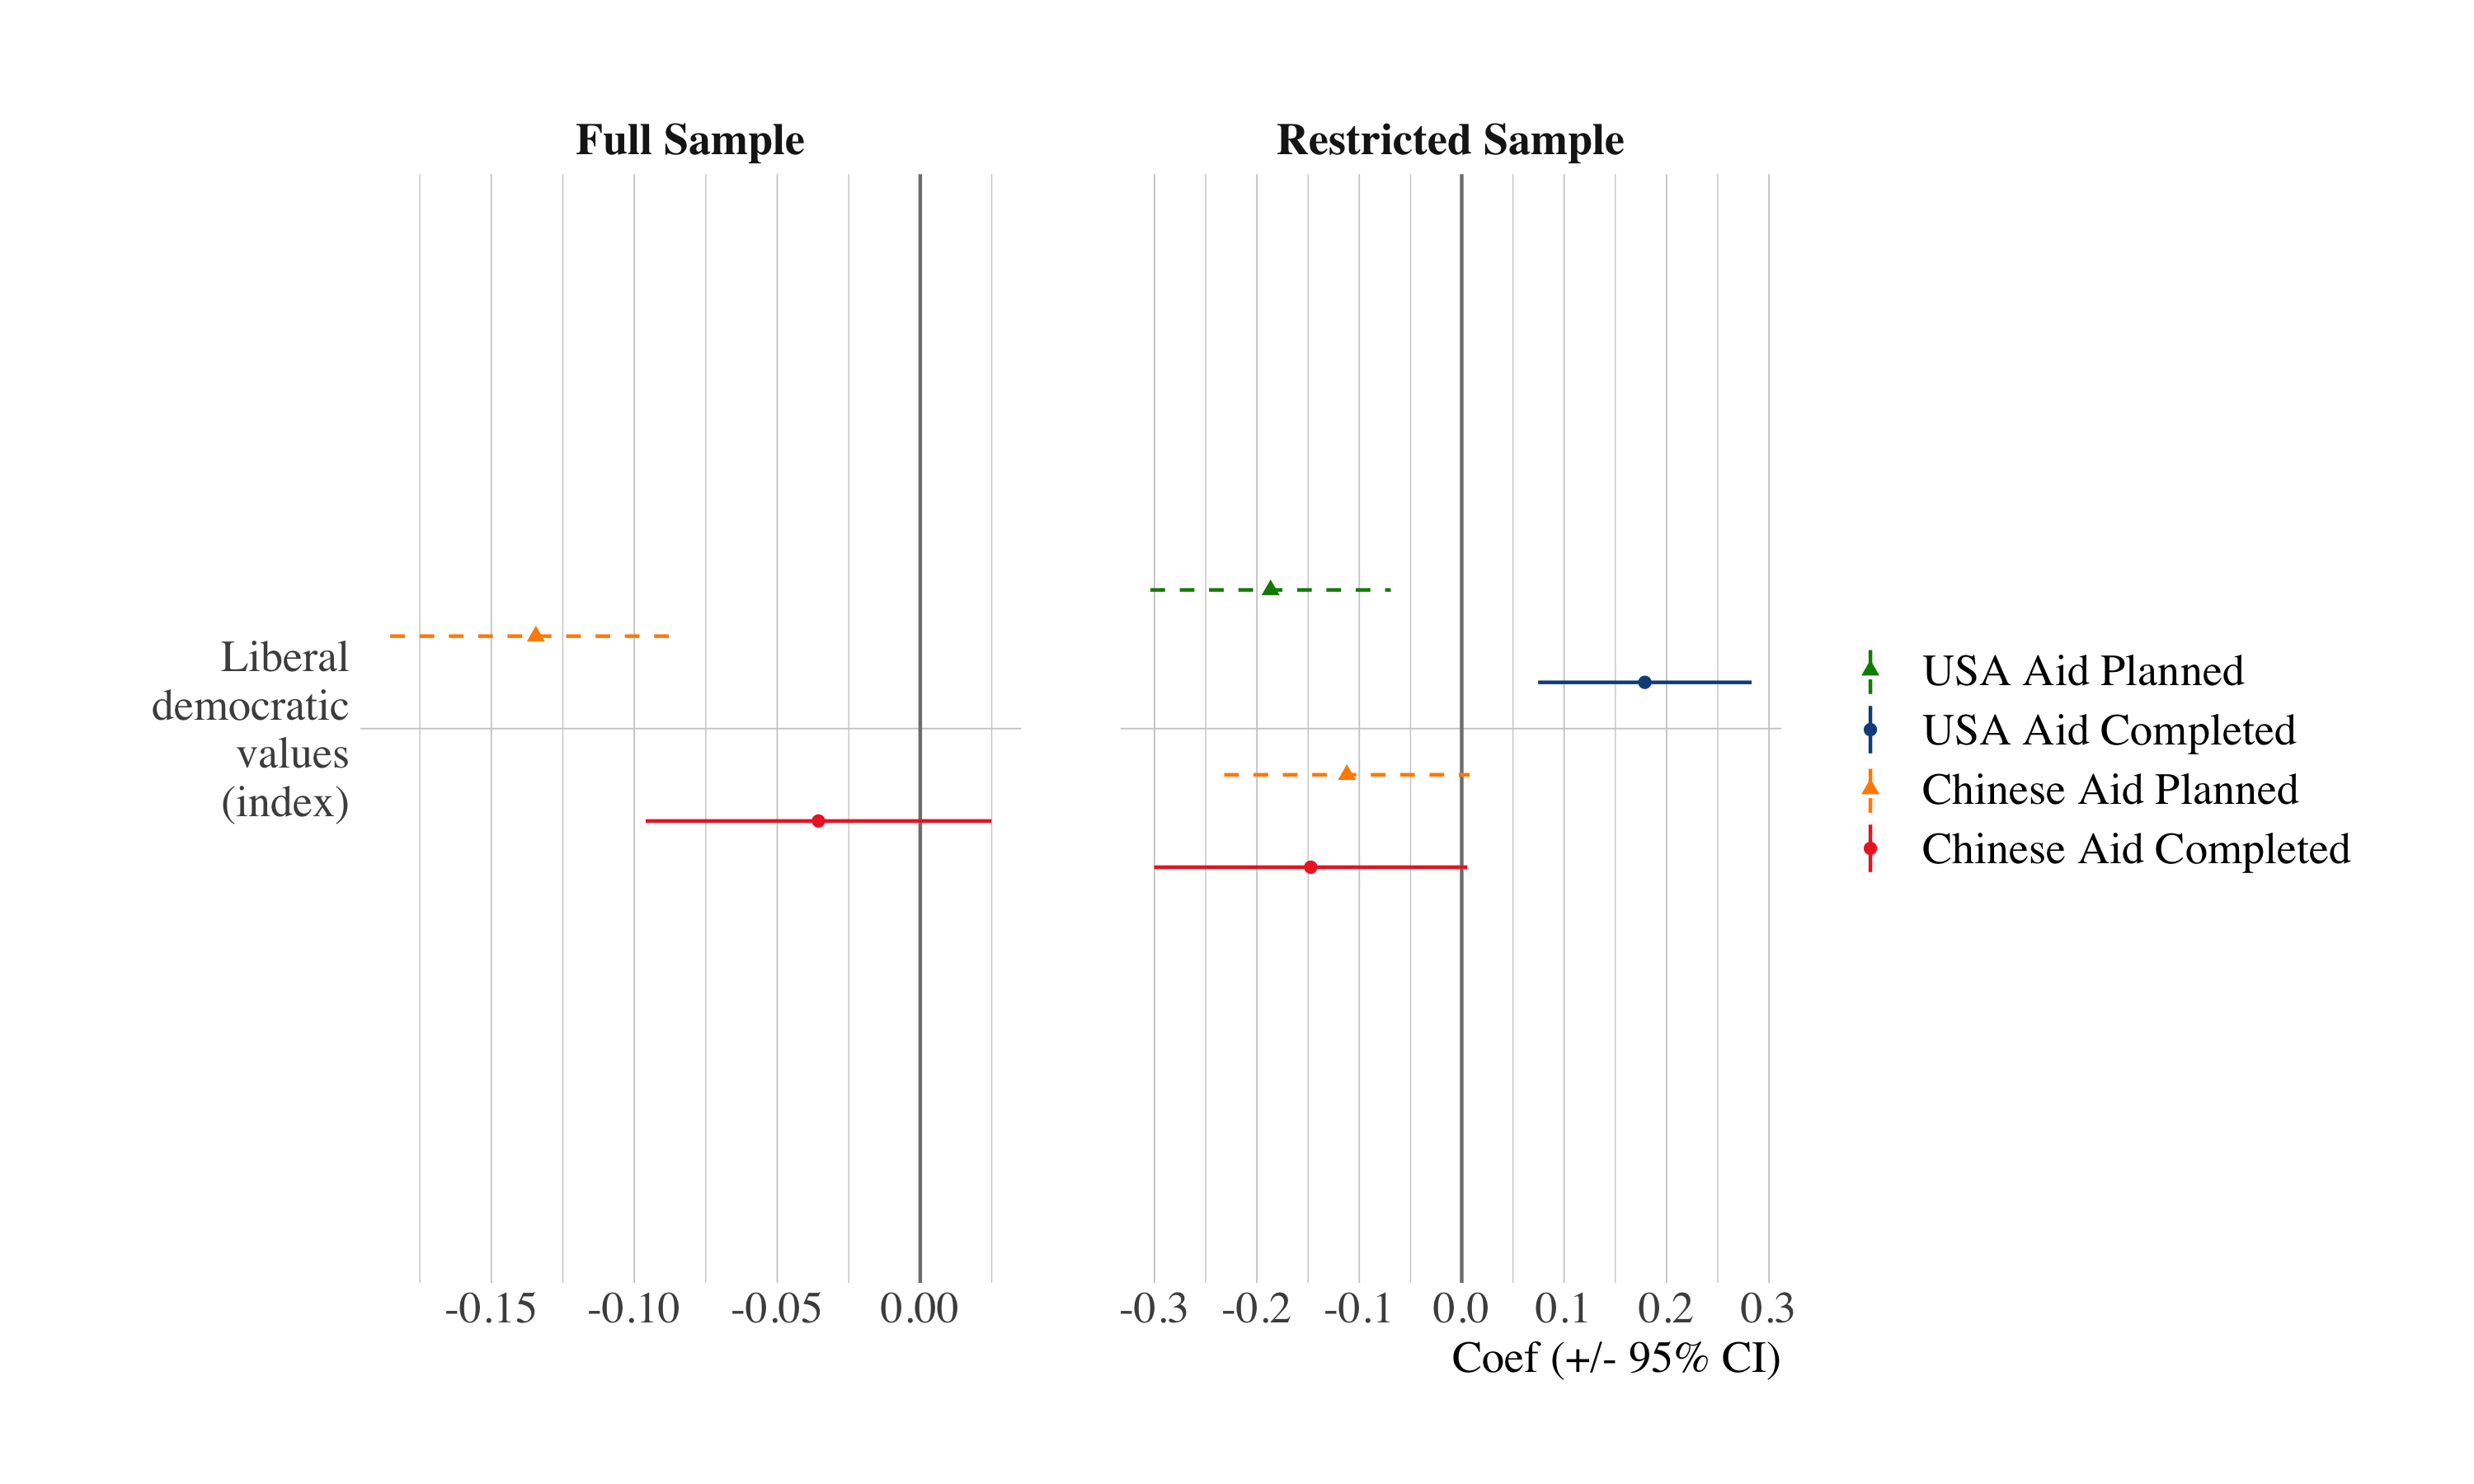
\includegraphics[width=1\textwidth]{figures/figure_a14.png}
\caption{Effects of Chinese and US aid on liberal democratic values, including additional controls}
\end{figure}

\begin{figure}[H]
\centering
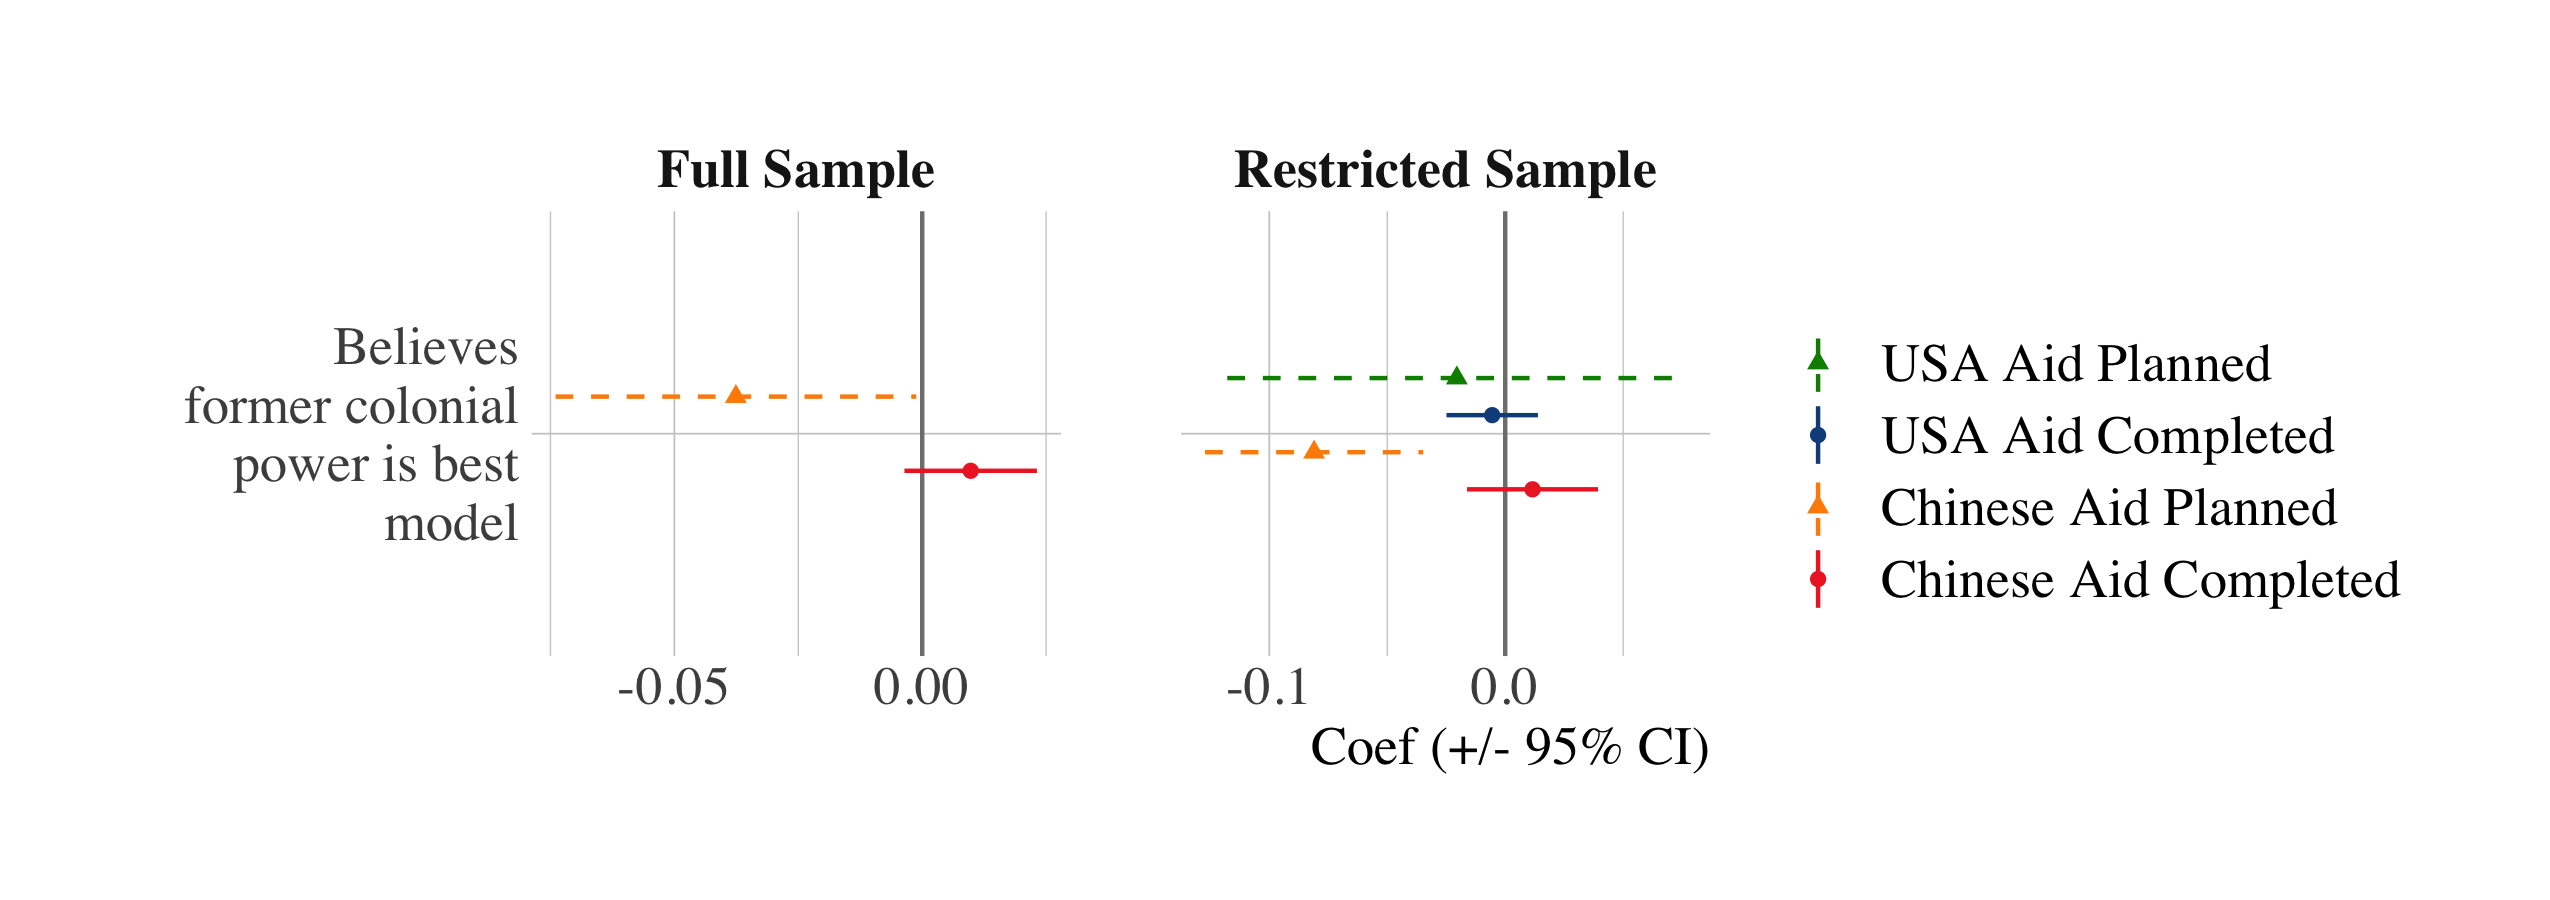
\includegraphics[width=1\textwidth]{figures/figure_a15.png}
\caption{Effects of Chinese and US aid on perceptions of former colonial powers, including additional controls}
\end{figure}

\newpage %% 

\setlength{\tabcolsep}{5pt}
\begin{table}[H]
\caption{Effects of Chinese aid on perceptions of China and the US, including spatial lag of DV}
\label{reg}
\centering
\import{tables/}{table_a9.tex}
\end{table}

\setlength{\tabcolsep}{5pt}
\begin{table}[H]
\caption{Effects of Chinese and US aid on perceptions of China and the US, including spatial lag of DV}
\label{reg}
\centering
\import{tables/}{table_a10.tex}
\end{table}

\newpage %% 

\setlength{\tabcolsep}{5pt}
\begin{table}[H]
\caption{Effects of Chinese aid on liberal democratic values, including spatial lag of DV}
\label{reg}
\centering
\import{tables/}{table_a11.tex}
\end{table}

\setlength{\tabcolsep}{5pt}
\begin{table}[H]
\caption{Effects of Chinese and US aid on liberal democratic values, including spatial lag of DV}
\label{reg}
\centering
\import{tables/}{table_a12.tex}
\end{table}

\newpage %% 

\setlength{\tabcolsep}{5pt}
\begin{table}[H]
\caption{Effects of Chinese aid on perceptions of former colonial powers, including spatial lag of DV}
\label{reg}
\centering
\import{tables/}{table_a13.tex}
\end{table}

\setlength{\tabcolsep}{5pt}
\begin{table}[H]
\caption{Effects of Chinese and US aid on perceptions of former colonial powers, including spatial lag of DV}
\label{reg}
\centering
\import{tables/}{table_a14.tex}
\end{table}

% ------------------------------------------------------------------------------------
\newpage
\section{Appendix 3: Extensions}

\begin{figure}[H]
\centering
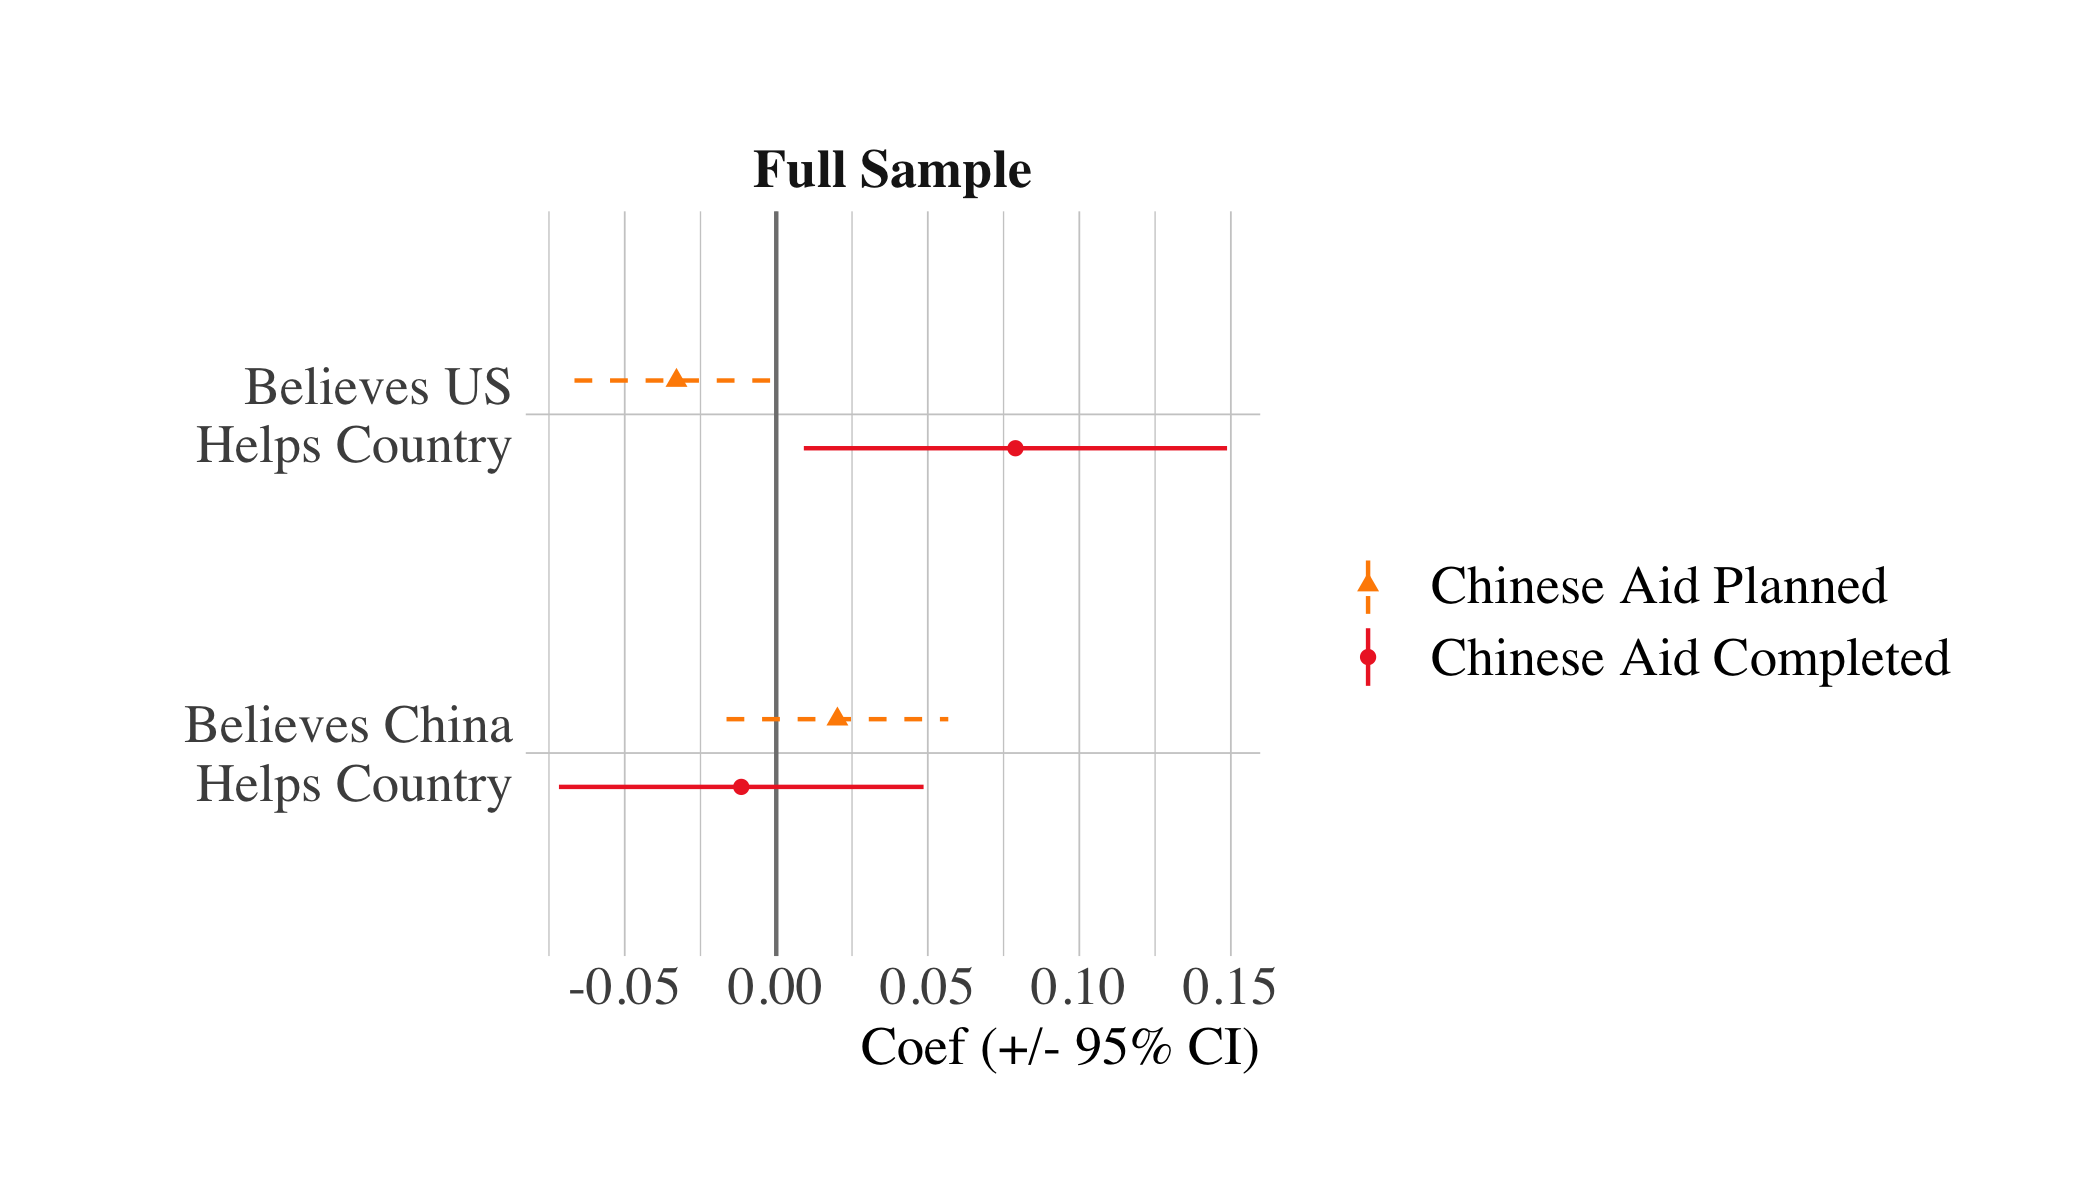
\includegraphics[width=0.8\textwidth]{figures/figure_a16.png}
\caption{Effects of Chinese aid on perceptions of China and the US, using round 4 only}
\end{figure}

\begin{figure}[H]
\centering
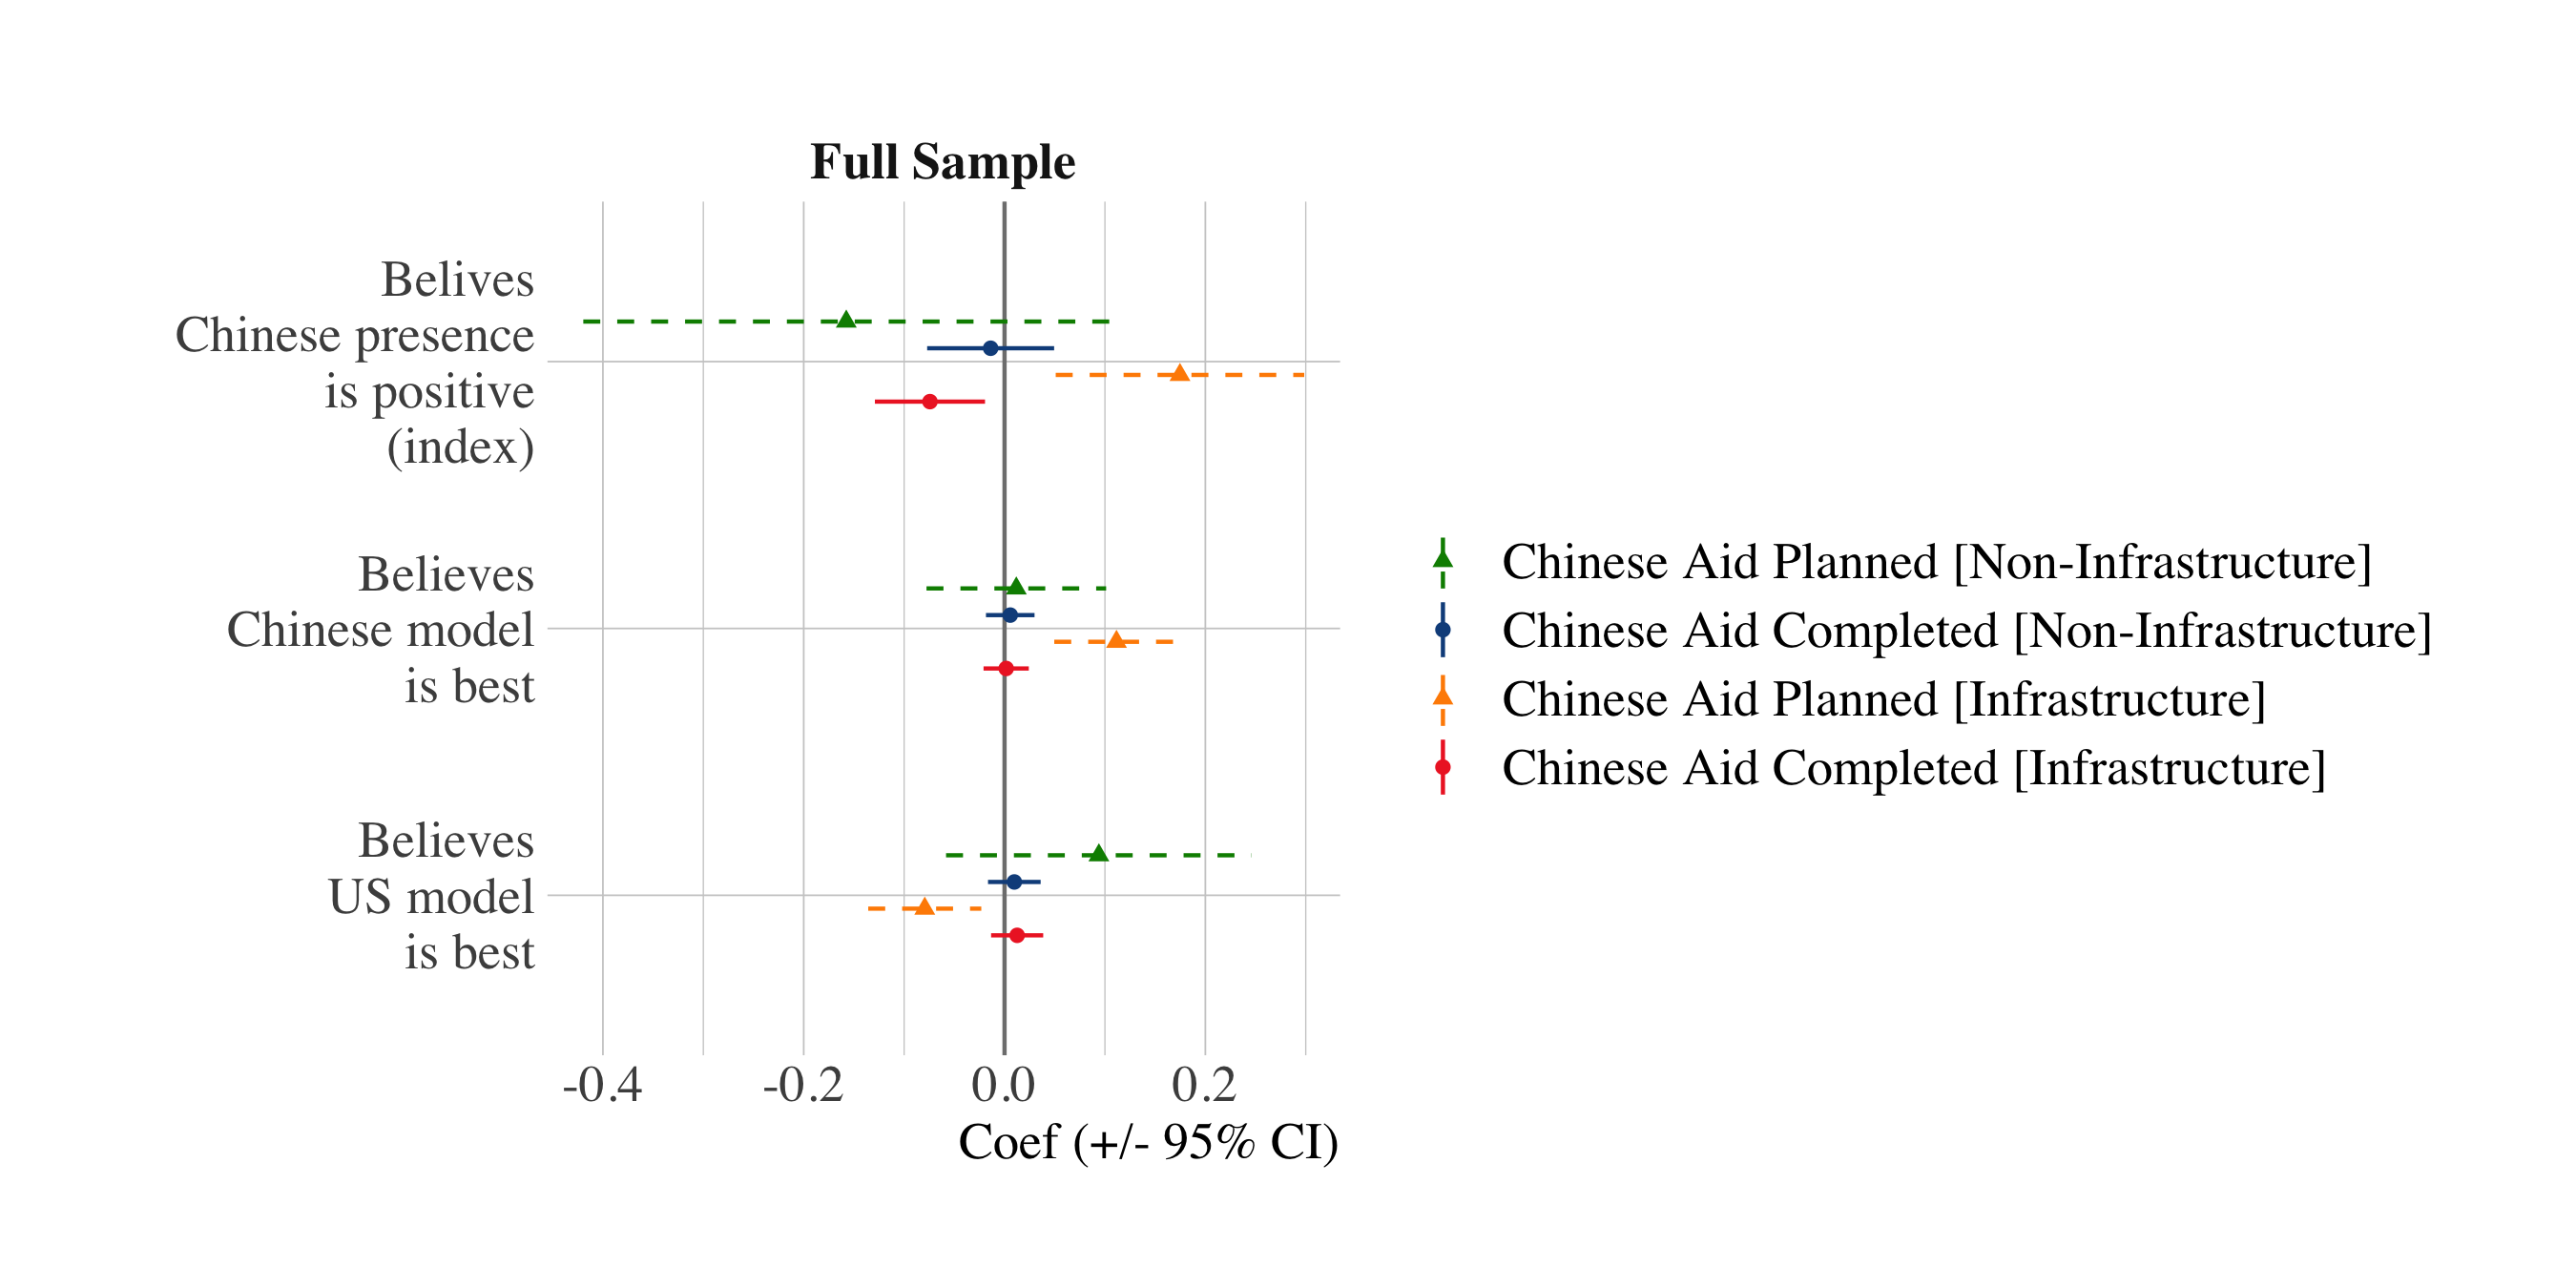
\includegraphics[width=1\textwidth]{figures/figure_a17.png}
\caption{Effects of Chinese aid on perceptions of China and the US, disaggregating by sector}
\end{figure}

\begin{figure}[H]
\centering
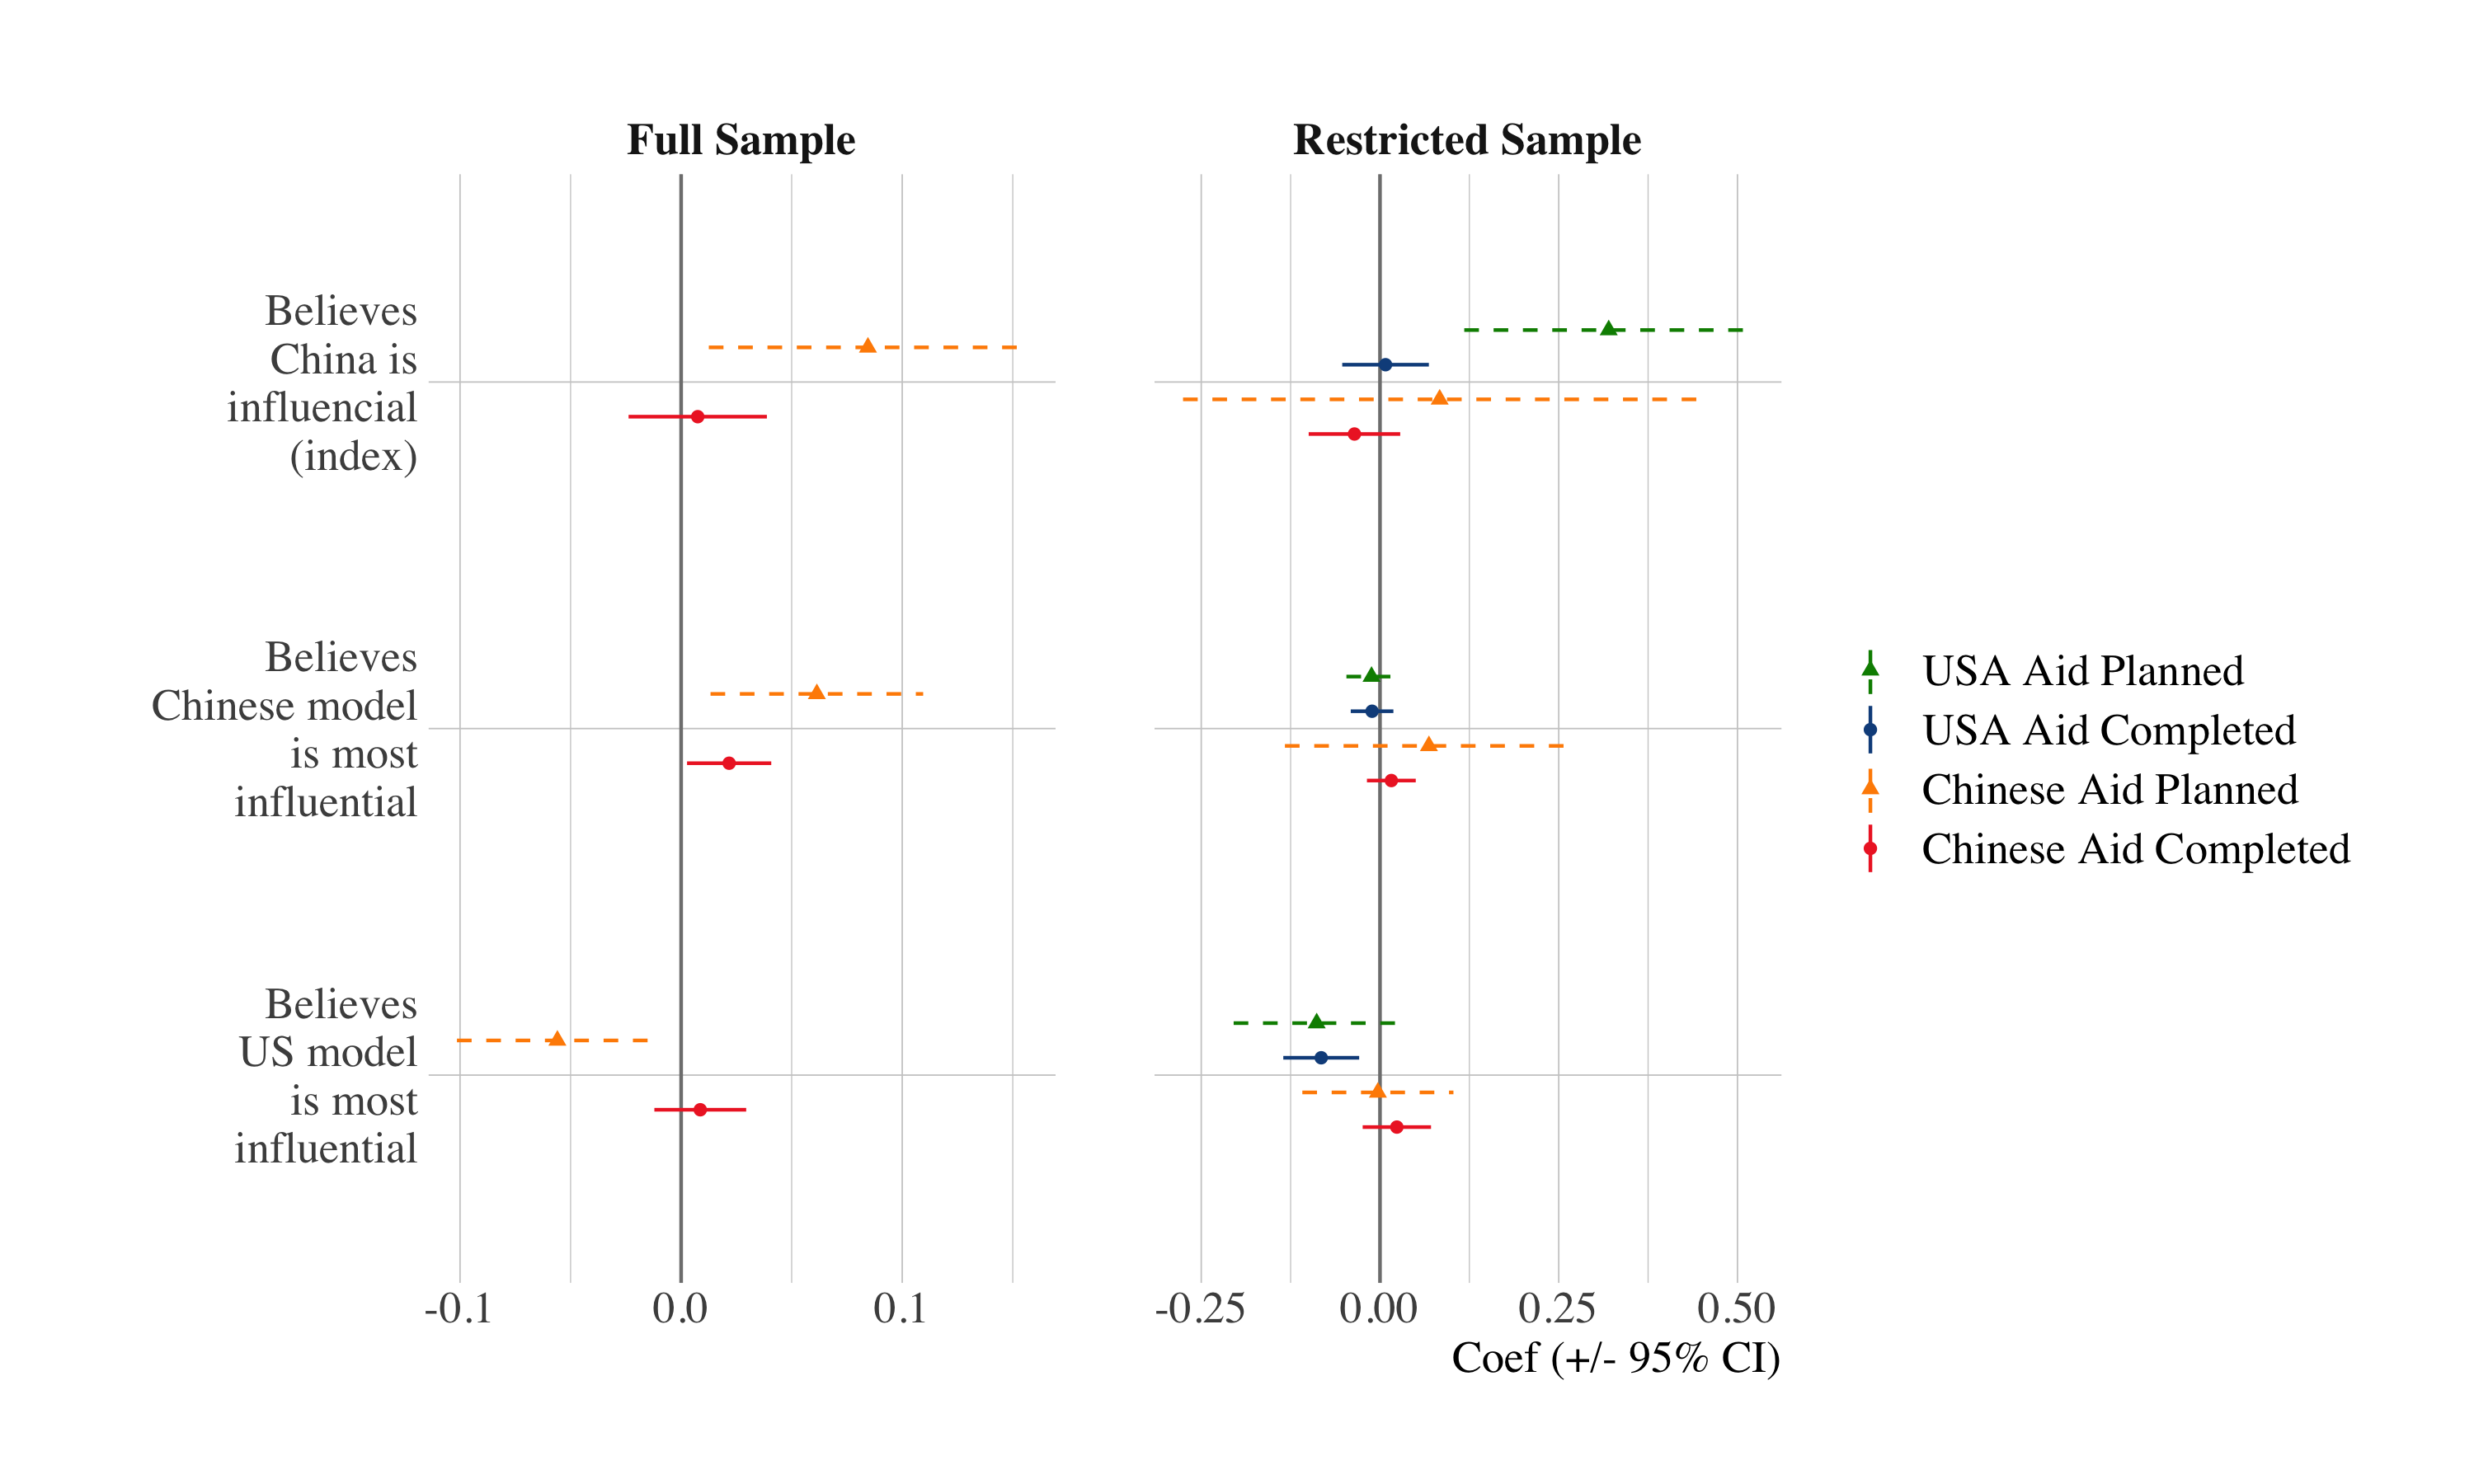
\includegraphics[width=1\textwidth]{figures/figure_a18.png}
\caption{Effects of Chinese and US aid on perceptions of Chinese and US influence}
\end{figure}

\begin{figure}[H]
\centering
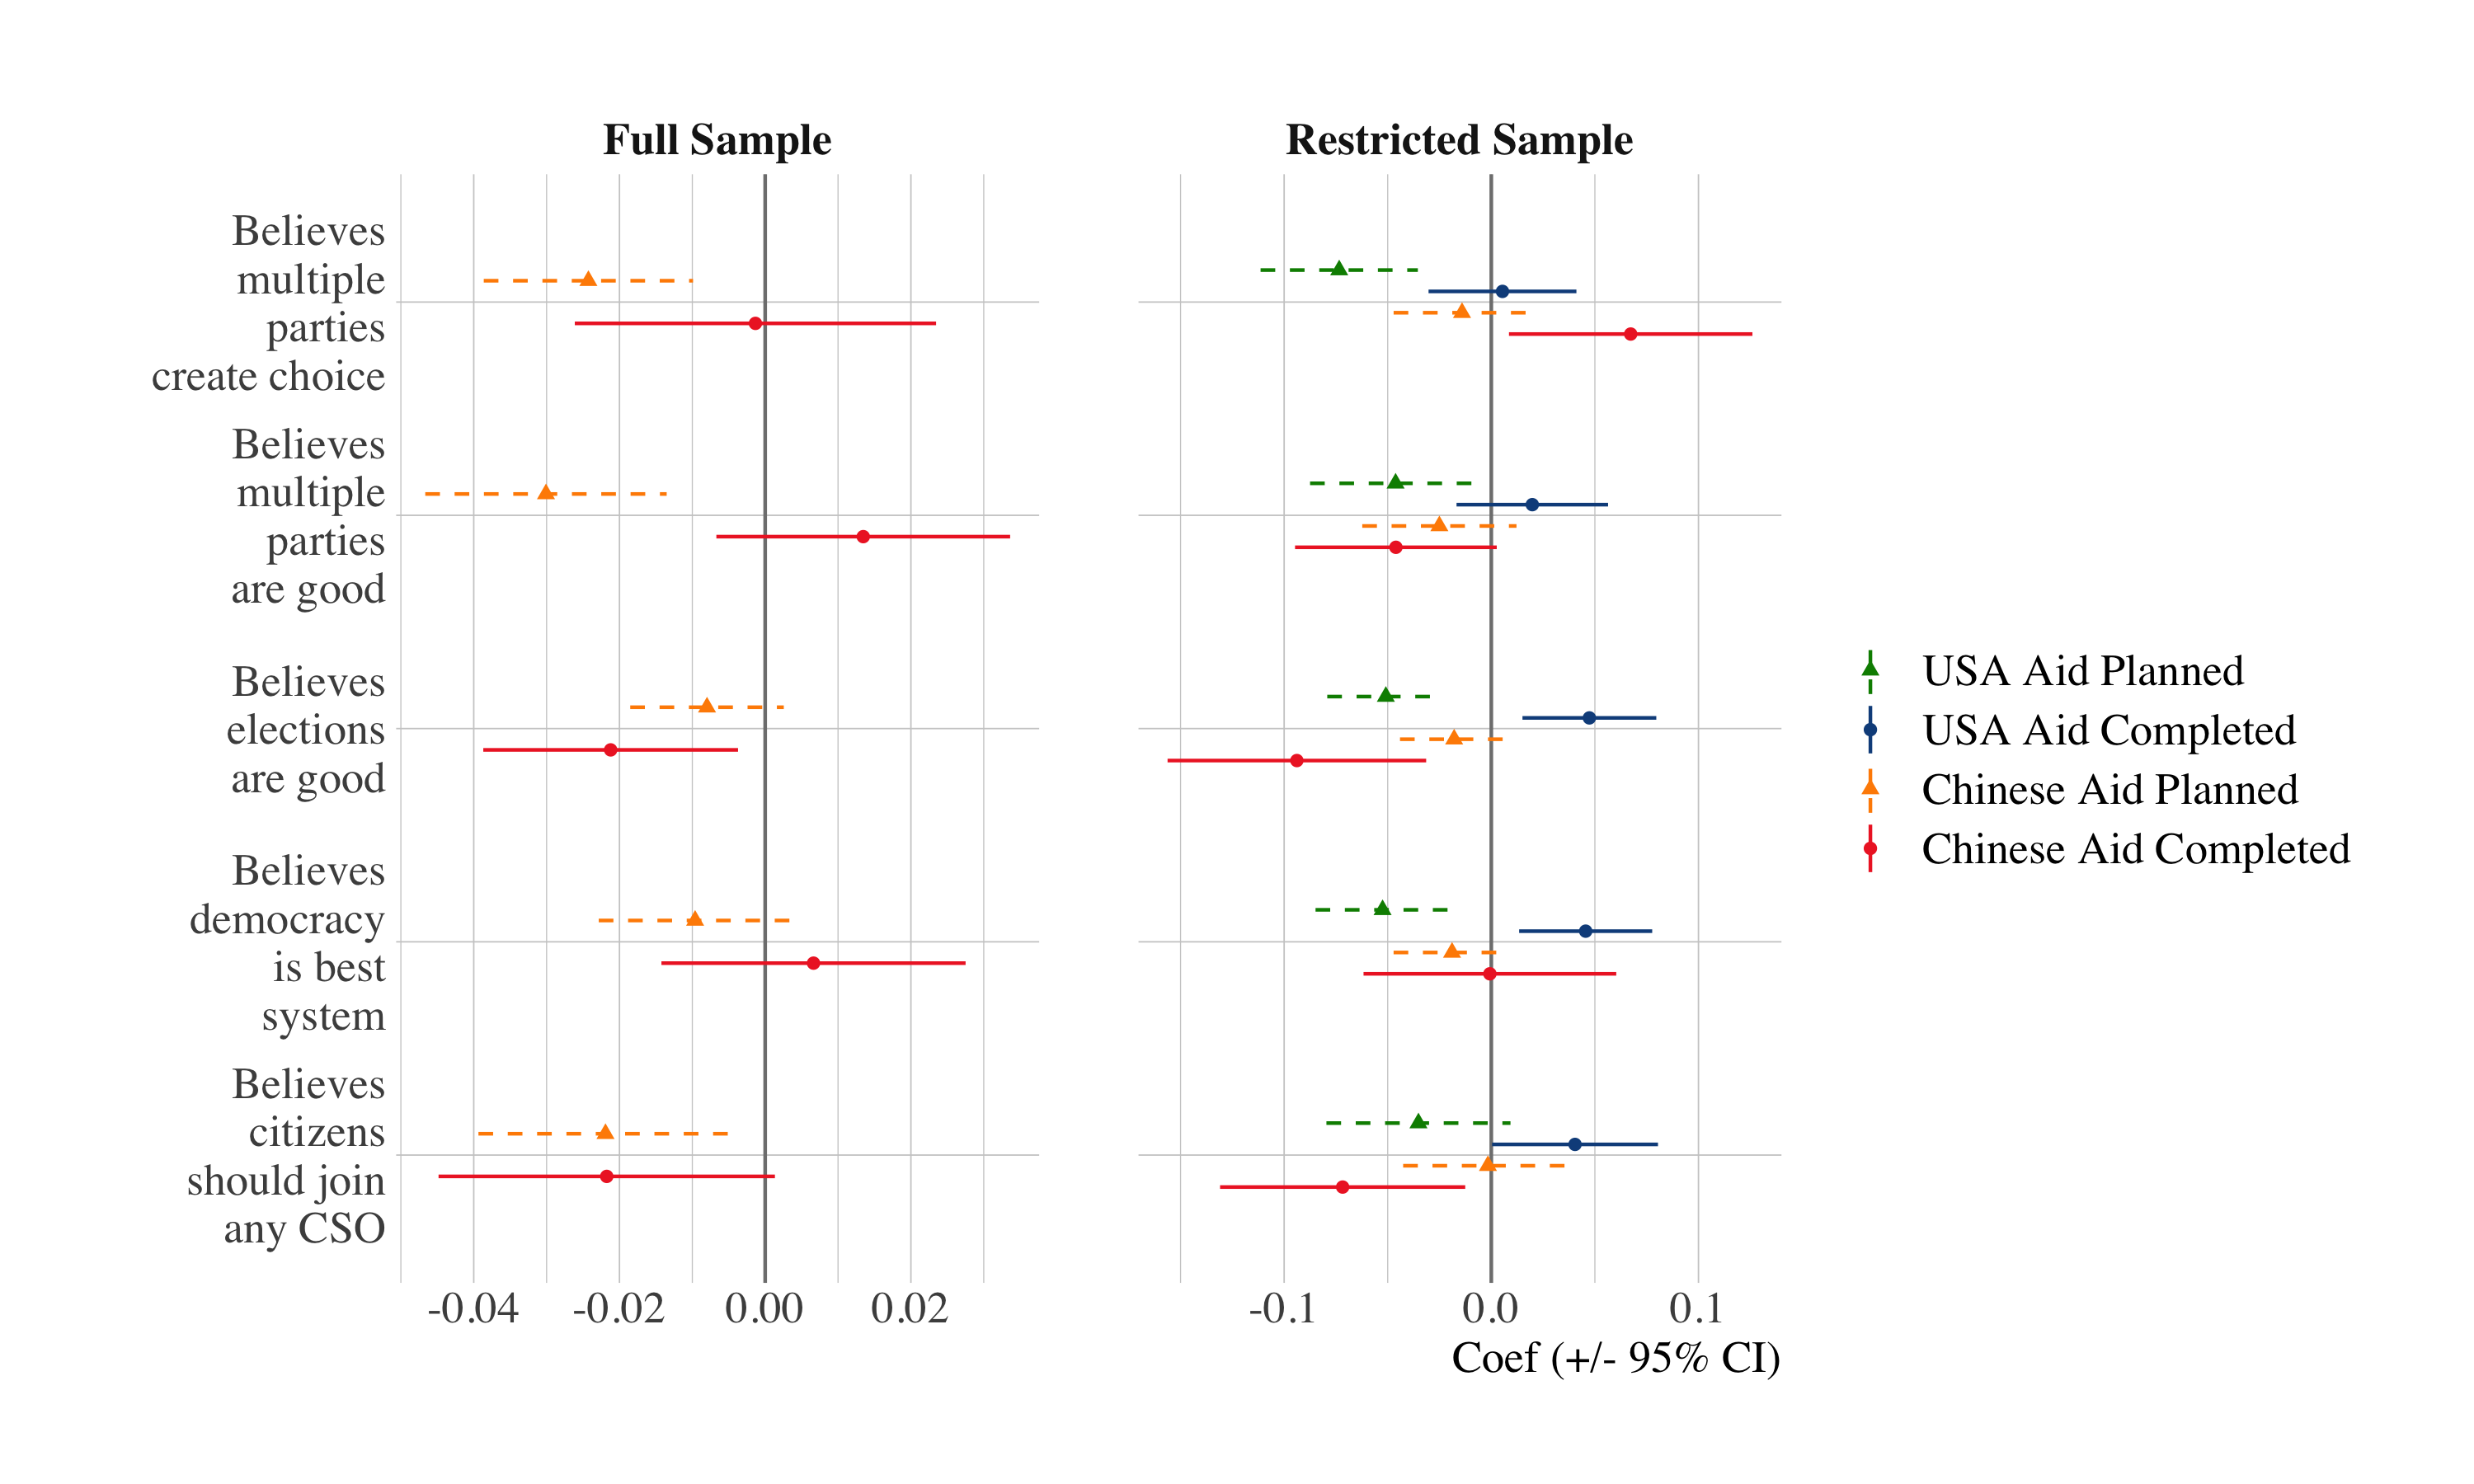
\includegraphics[width=1\textwidth]{figures/figure_a19.png}
\caption{Effects of Chinese and US aid on disaggregated liberal democratic values}
\end{figure}

\begin{figure}[H]
\centering
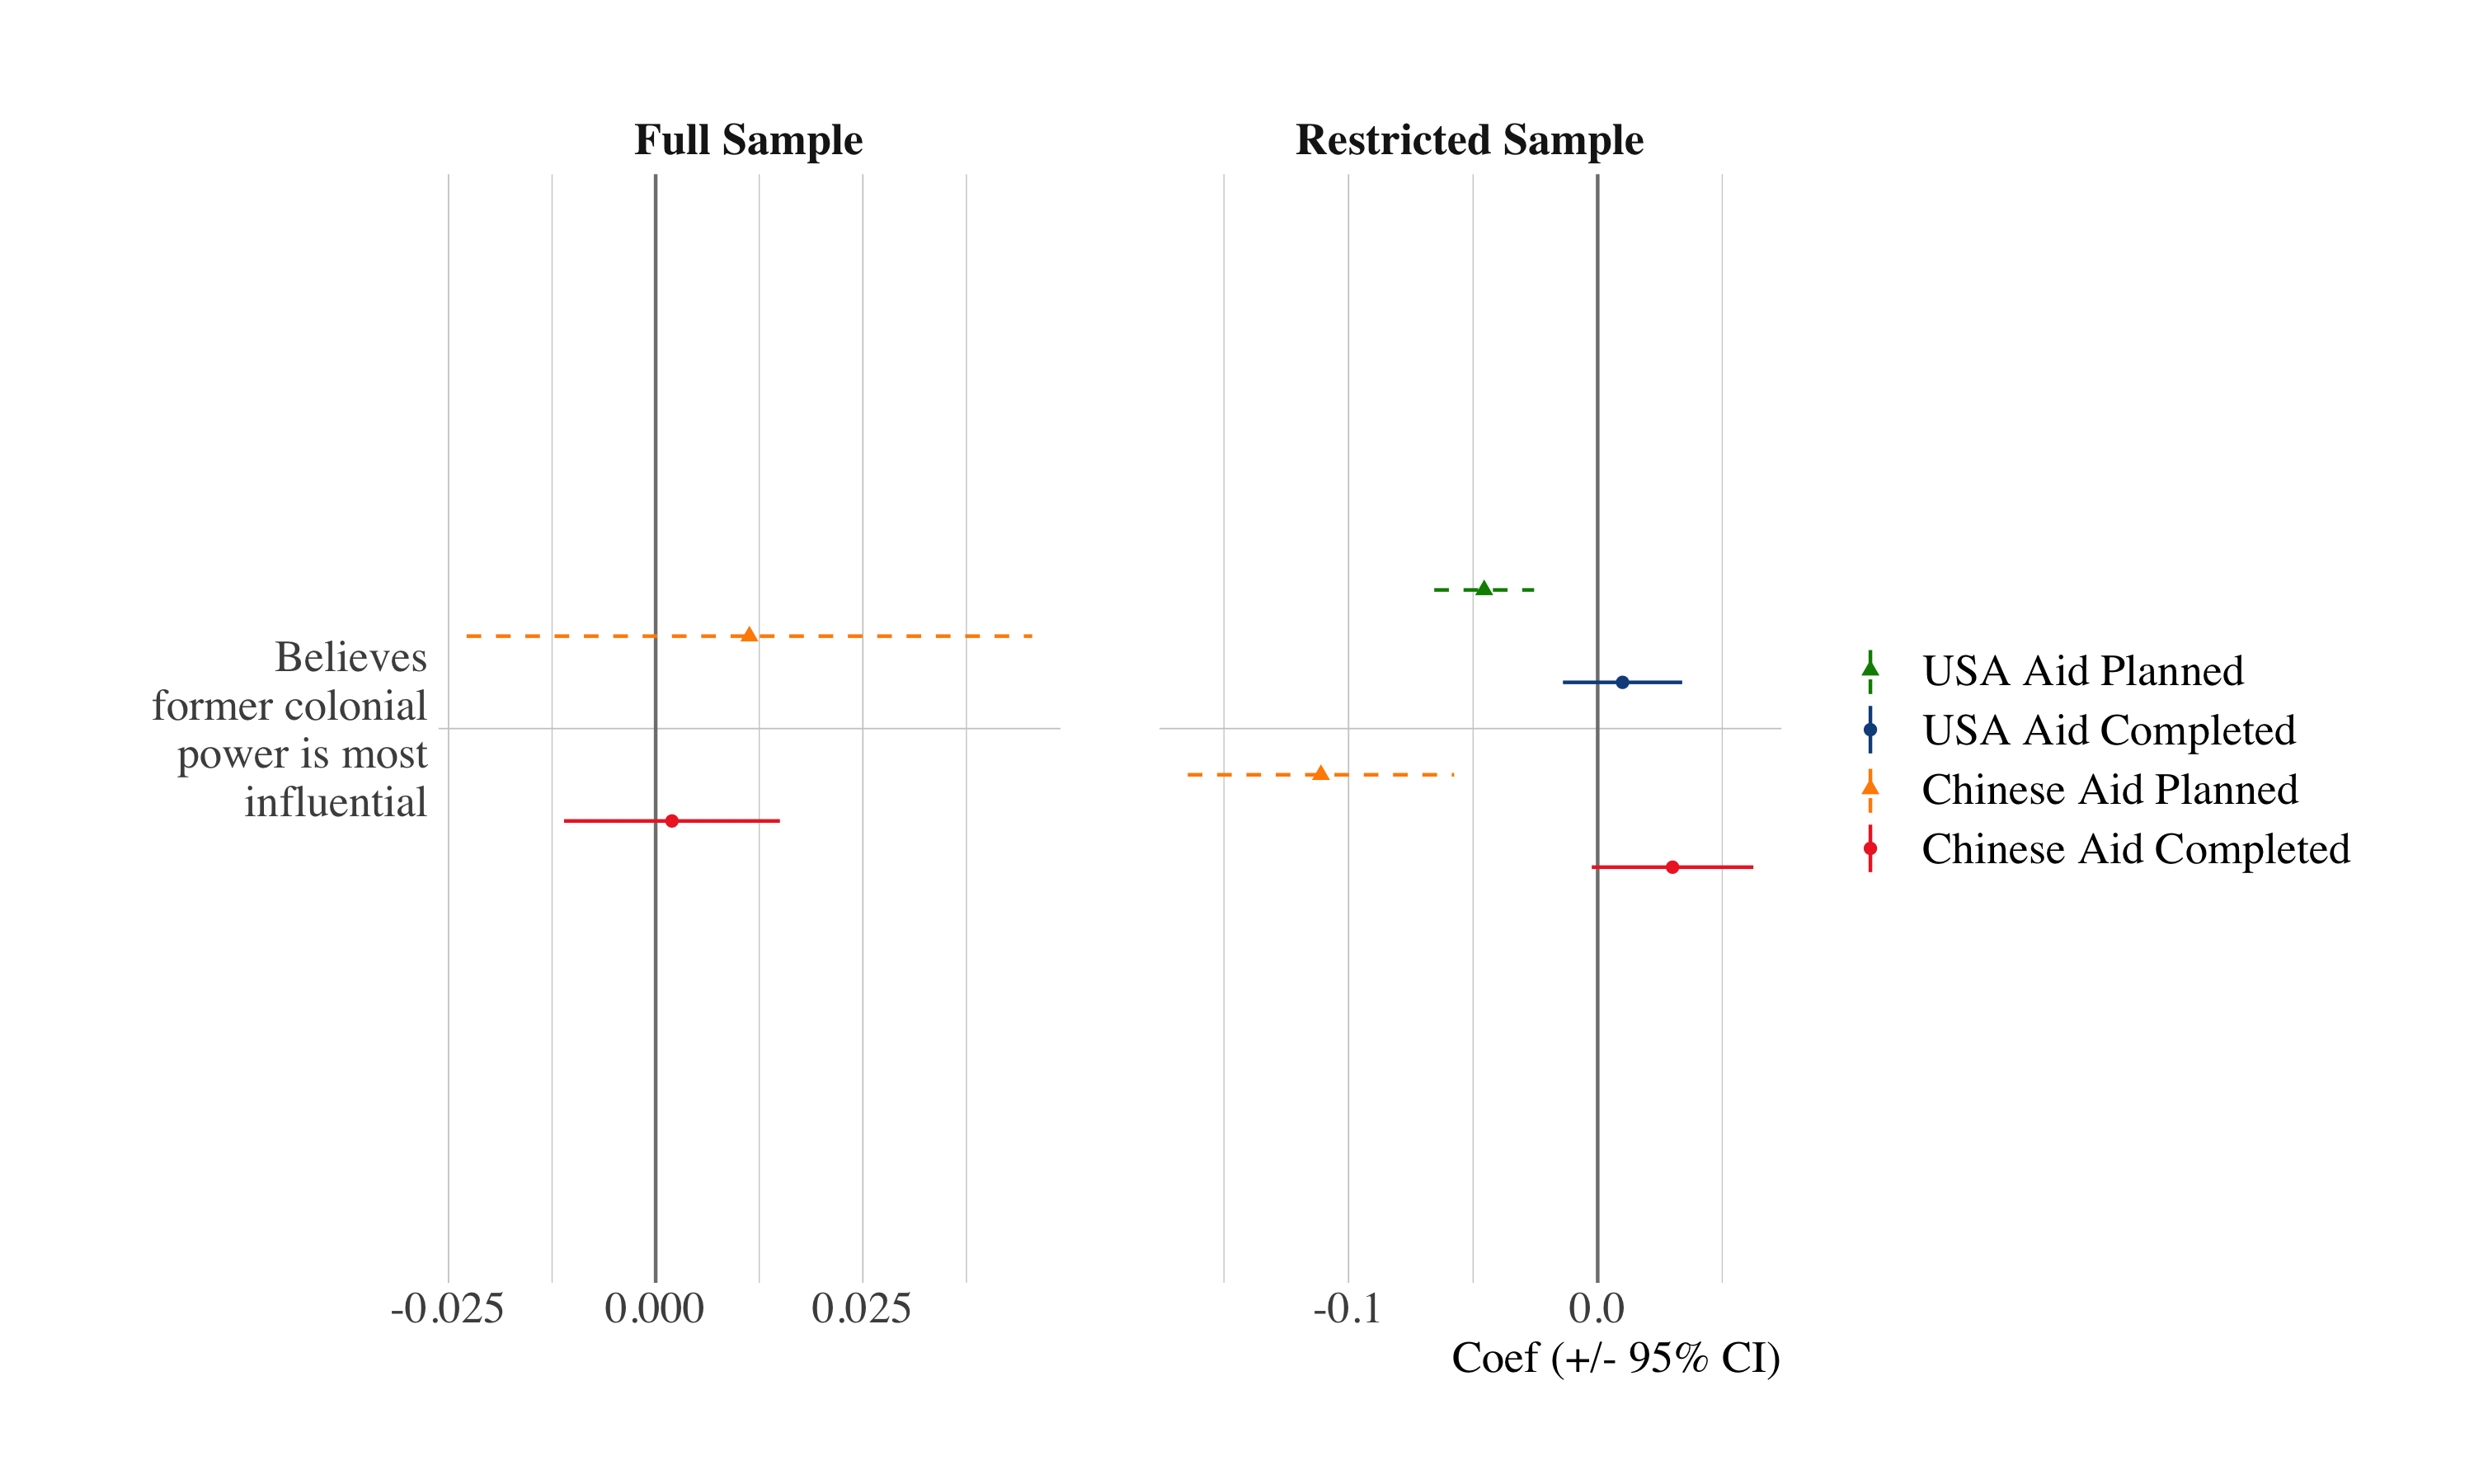
\includegraphics[width=1\textwidth]{figures/figure_a20.png}
\caption{Effects of Chinese and US aid on perceptions of former colonial powers' influence}
\end{figure}

\begin{figure}[H]
\centering
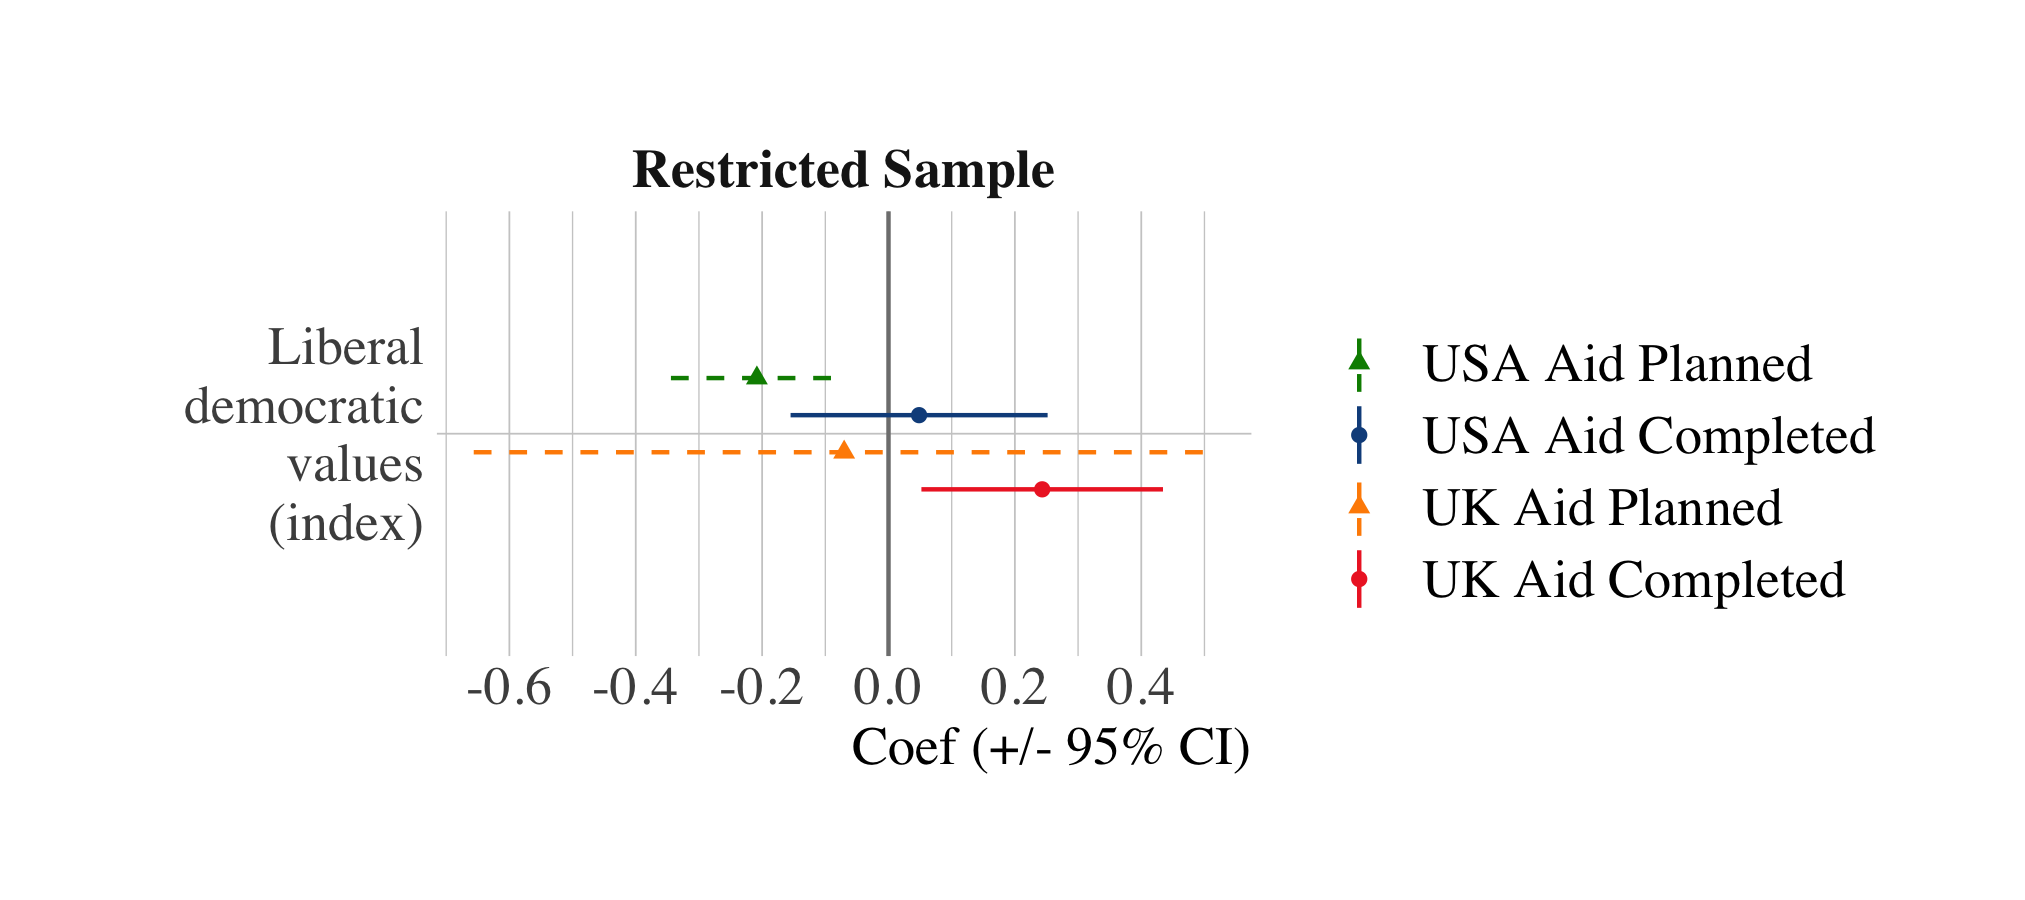
\includegraphics[width=0.8\textwidth]{figures/figure_a21.png}
\caption{Effects of US and UK aid on liberal democratic values}
\end{figure}

\end{document}  
















